\documentclass[serif]{beamer}

\def\gridopacity{100}
\def\gridopacity{0}

\usepackage{multimedia}

% see http://tex.stackexchange.com/a/24491
% for how to use enumitem with beamer
\usepackage{enumitem}
\setitemize{label=\usebeamerfont*{itemize item}%
  \usebeamercolor[fg]{itemize item}
  \usebeamertemplate{itemize item}}

% default page size is:
% \beamer@paperwidth 12.80cm%
% \beamer@paperheight 9.60cm%

\setbeamersize{text margin left=0.4cm,text margin right=0.4cm}

\usepackage{tikz}
\usetikzlibrary{calc,decorations.pathreplacing,positioning}
\usepackage{pgfplots}

\usepackage[clock,misc]{ifsym} % for \showclock

% pretty tables
\usepackage{multirow}
\usepackage{booktabs}

% this is from http://tex.stackexchange.com/a/103691
% taken from manual
\makeatletter
\pgfdeclareshape{document}{
\inheritsavedanchors[from=rectangle] % this is nearly a rectangle
\inheritanchorborder[from=rectangle]
\inheritanchor[from=rectangle]{center}
\inheritanchor[from=rectangle]{north}
\inheritanchor[from=rectangle]{south}
\inheritanchor[from=rectangle]{west}
\inheritanchor[from=rectangle]{east}
% ... and possibly more
\backgroundpath{% this is new
% store lower right in xa/ya and upper right in xb/yb
\southwest \pgf@xa=\pgf@x \pgf@ya=\pgf@y
\northeast \pgf@xb=\pgf@x \pgf@yb=\pgf@y
% compute corner of ‘‘flipped page’’
\pgf@xc=\pgf@xb \advance\pgf@xc by-10pt % this should be a parameter
\pgf@yc=\pgf@yb \advance\pgf@yc by-10pt
% construct main path
\pgfpathmoveto{\pgfpoint{\pgf@xa}{\pgf@ya}}
\pgfpathlineto{\pgfpoint{\pgf@xa}{\pgf@yb}}
\pgfpathlineto{\pgfpoint{\pgf@xc}{\pgf@yb}}
\pgfpathlineto{\pgfpoint{\pgf@xb}{\pgf@yc}}
\pgfpathlineto{\pgfpoint{\pgf@xb}{\pgf@ya}}
\pgfpathclose
% add little corner
\pgfpathmoveto{\pgfpoint{\pgf@xc}{\pgf@yb}}
\pgfpathlineto{\pgfpoint{\pgf@xc}{\pgf@yc}}
\pgfpathlineto{\pgfpoint{\pgf@xb}{\pgf@yc}}
\pgfpathlineto{\pgfpoint{\pgf@xc}{\pgf@yc}}
}
}
\makeatother

\usepackage{algorithm}
\usepackage[noend]{algpseudocode}

% symbols
\usepackage{amsmath} % assumes amsmath package installed
\usepackage{amssymb} % for \square
% non-italicized math subscripts
\newcommand{\ms}[1]{\mbox{\scriptsize #1}}
% from http://tex.stackexchange.com/a/5255
\DeclareMathOperator*{\argmin}{arg\,min}

% fonts
\renewcommand\rmdefault{pplx}
\renewcommand\mathfamilydefault{cmr}

\setbeamertemplate{navigation symbols}{}

\setbeamerfont{page number in head/foot}{size=\large}
%\setbeamertemplate{footline}[frame number]
\setbeamertemplate{footline}{%
   \raisebox{7pt}{\makebox[\paperwidth]{%
   \hfill\makebox[10pt]{\textcolor{gray}{%
   \large\insertframenumber\hspace{0.1in}}}}}}

% dont number title page
\addtocounter{framenumber}{-1}

\title{Efficient Manipulation Task Planning via
Reuse-Informed Optimization of Planning Effort}
\author{Christopher M. Dellin}
\date{April 7, 2015}

\begin{document}

\begin{frame}[plain]
   %\begin{columns}
   %   \column{1.2\textwidth}
      \maketitle
   %\end{columns}
\end{frame}

% first frame:
% REAL ROBOTS! REAL-WORLD PROBLEMS!
% overview of manipulation planning problem?
\begin{frame}
   \frametitle{Autonomous Manipulation Tasks}
   \begin{tikzpicture}
      \draw[step=1,black!10,very thin,opacity=\gridopacity] (0,0) grid (12,8);
   
      \node[inner sep=0] at ( 2,5.0) {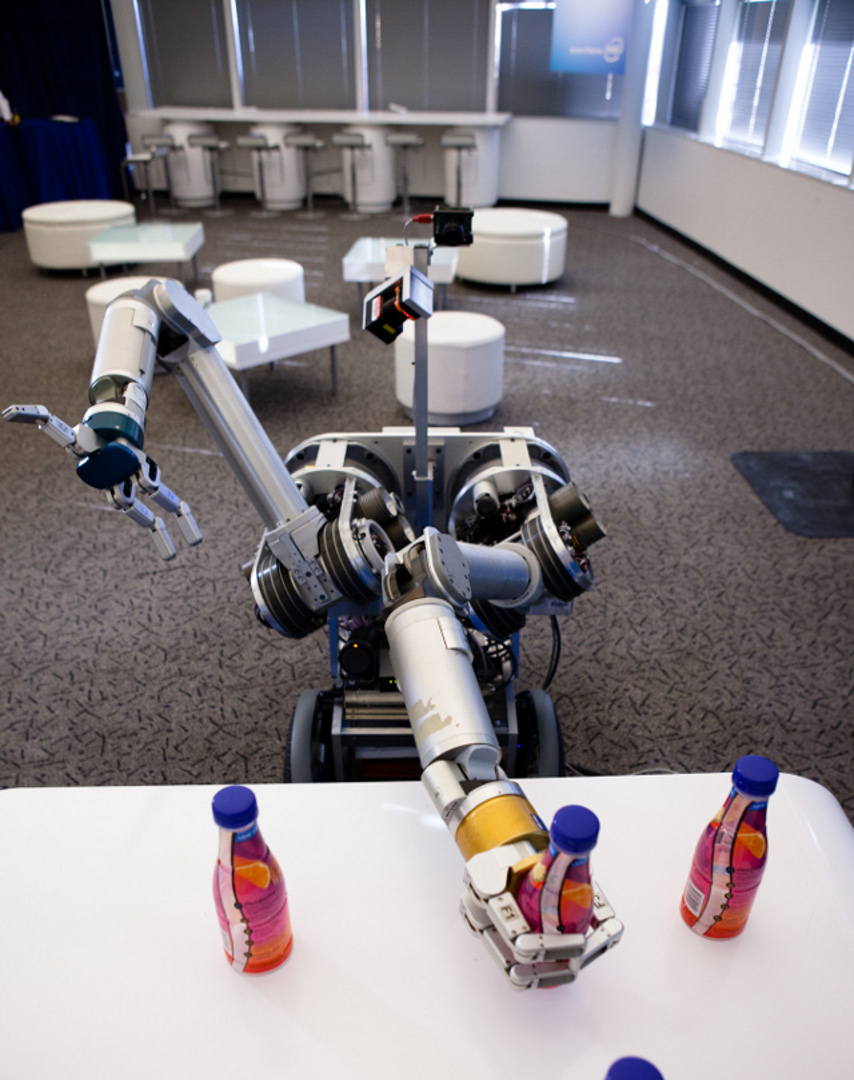
\includegraphics[width=3.5cm]{images/herb.jpg}};
      \node[inner sep=0] at ( 6,5.0) {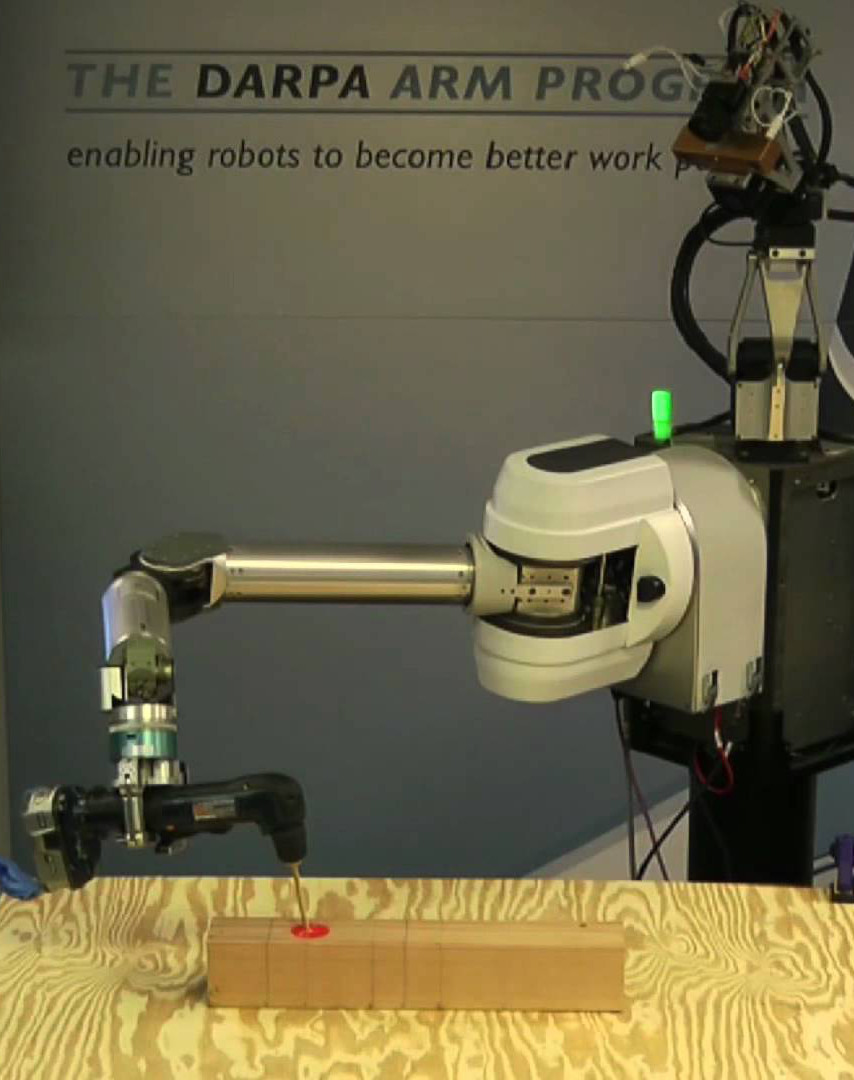
\includegraphics[width=3.5cm]{images/arms.jpg}};
      \node[inner sep=0] at (10,5.0) {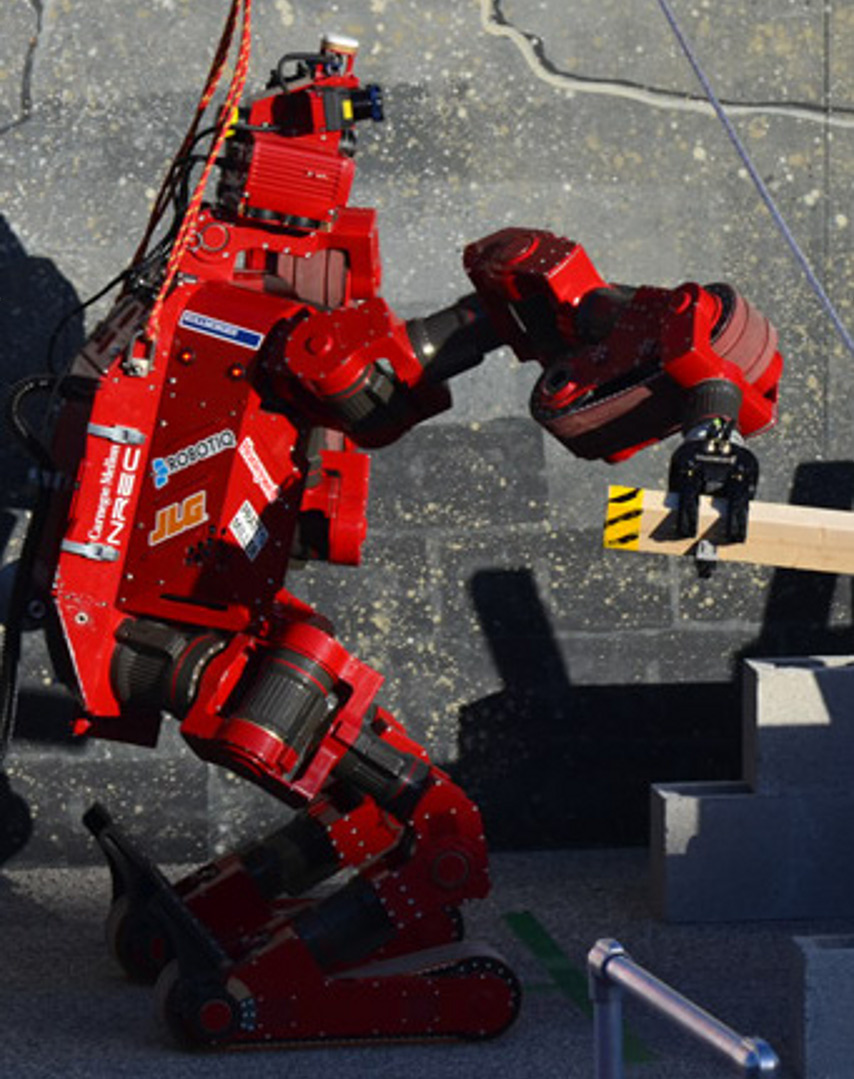
\includegraphics[width=3.5cm]{images/chimp.jpg}};
      \node at ( 2,2.4) {Herb};
      \node at ( 6,2.4) {ARM-S};
      \node at (10,2.4) {CHIMP};
      
      \begin{scope}[font=\footnotesize]
         \only<2->{
            \node[draw,align=center,minimum height=1.2cm,font=\tiny]
               (a) at (1,0.85) {Unknown\\Environment};
         }
         
         \only<3->{
            \node[fill=blue!10,rounded corners,align=center,minimum height=1.5cm]
               (b) at (3,0.85) {Onboard\\Sensors};
            \draw[->,line width=1pt] (a) -- (b);
         }
         
         \only<4->{
            \node[draw,align=center,minimum height=1.2cm,font=\tiny]
               (c) at (5,0.85) {Geometric\\World\\Model};
            \draw[->,line width=1pt] (b) -- (c);
         }
         
         \only<5->{
            \node[fill=blue!10,rounded corners,align=center,minimum height=1.5cm]
               (d) at (7,0.85) {Onboard\\Motion\\Planner};
            \draw[->,line width=1pt] (c) -- (d);
         }
         
         \only<6->{
            \node[draw,align=center,minimum height=1.2cm,font=\tiny]
               (e) at (9,0.85) {Motion};
               \draw[->,line width=1pt] (d) -- (e);
         }
         
         \only<7->{
            \node[fill=blue!10,rounded corners,align=center,minimum height=1.5cm]
               (f) at (11,0.85) {Motion\\Execution};
            \draw[->,line width=1pt] (e) -- (f);
         }
      \end{scope}
   
   \end{tikzpicture}
\end{frame}

\begin{frame}
   \frametitle{Example Manipulation Tasks}
   \begin{tikzpicture}
      \draw[step=1,black!10,very thin,opacity=\gridopacity] (0,0) grid (12,8);

      \node[fill=black,inner sep=1pt] at (3,6.3) {
         \movie[width=5.333333cm,height=3.00cm,
            loop,autostart]{}{chimp-trials-debris-fast.mp4}
      };
      
      \node[fill=black,inner sep=1pt] at (9,6.3) {
         \movie[width=5.333333cm,height=3.00cm,
            loop,autostart]{}{herb-tableclear-2-fast.mp4}
      };
      
      \node[fill=black,minimum width=4cm, minimum height=3cm,text=white] at (3,3.2) {
         ARM-S Example?
      };
      
      \node[fill=black,minimum width=4cm, minimum height=3cm,text=white] at (9,3.2) {
         Other (PR-2) Example?
      };
   
      %\hyperlinkmovie[play]{mylabel}{play}

      \begin{scope}[font=\footnotesize]
         \node[draw,align=center,minimum height=1.2cm,font=\tiny]
            (a) at (1,0.85) {Unknown\\Environment};
         \node[fill=blue!10,rounded corners,align=center,minimum height=1.5cm]
            (b) at (3,0.85) {Onboard\\Sensors};
         \draw[->,line width=1pt] (a) -- (b);
         \node[draw,align=center,minimum height=1.2cm,font=\tiny]
            (c) at (5,0.85) {Geometric\\World\\Model};
         \draw[->,line width=1pt] (b) -- (c);
         \only<1>{
            \node[fill=blue!10,rounded corners,align=center,minimum height=1.5cm]
               (d) at (7,0.85) {Onboard\\Motion\\Planner};
         }
         \only<2>{
            \node[fill=green!20,rounded corners,align=center,minimum height=1.5cm]
               (d) at (7,0.85) {Onboard\\Motion\\Planner};
         }
         \draw[->,line width=1pt] (c) -- (d);
         \node[draw,align=center,minimum height=1.2cm,font=\tiny]
            (e) at (9,0.85) {Motion};
            \draw[->,line width=1pt] (d) -- (e);
         \node[fill=blue!10,rounded corners,align=center,minimum height=1.5cm]
            (f) at (11,0.85) {Motion\\Execution};
         \draw[->,line width=1pt] (e) -- (f);
      \end{scope}

   \end{tikzpicture}
\end{frame}

%\begin{frame}
%   \frametitle{tasks are slow because planning is slow}
%   
%   Make figure:
%   \begin{tabular}{ll}
%      HERB pic & 50\% planning time, 50\% exec time \\
%      CHIMP pic & 40\% planning time, 60\% exec time \\
%   \end{tabular}
%   
%   \medskip
%   Focus on planning for manipulation tasks.
%   Talk about WHY planning is slow, and WHY planning is necesary
%   in these problems.
%   
%   \medskip
%   Do I need this slide?
%\end{frame}

\begin{frame}
   \frametitle{3 Challenges to Efficient Manipulation Planning}
   \begin{tikzpicture}
      \draw[step=1,black!10,very thin,opacity=\gridopacity] (0,0) grid (12,8);

   \node[inner sep=0pt] at (6,5.3) {%
      \only<1-2>{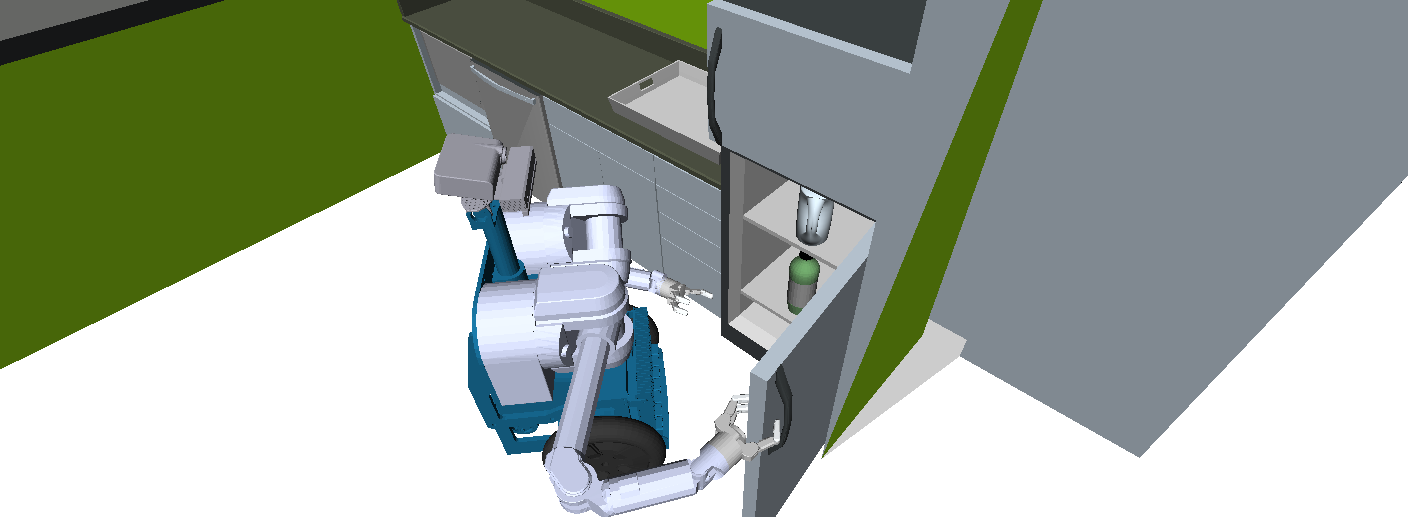
\includegraphics[width=11.5cm]{figs/herb-fridge-a.png}}%
      \only<3>{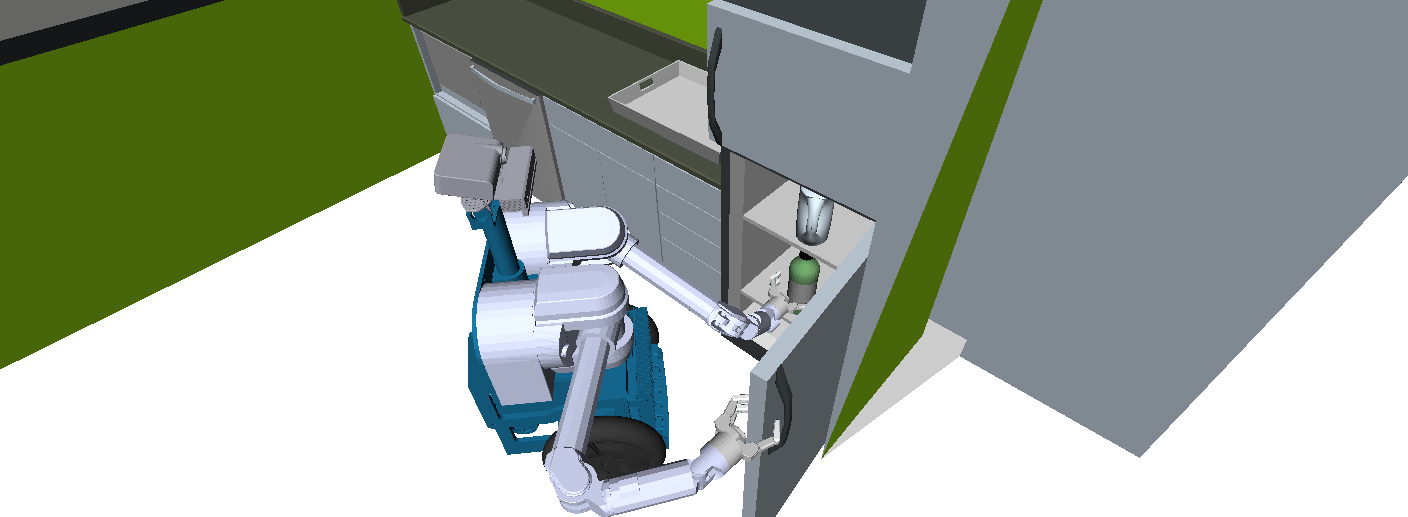
\includegraphics[width=11.5cm]{figs/herb-fridge-b.png}}%
      \only<4>{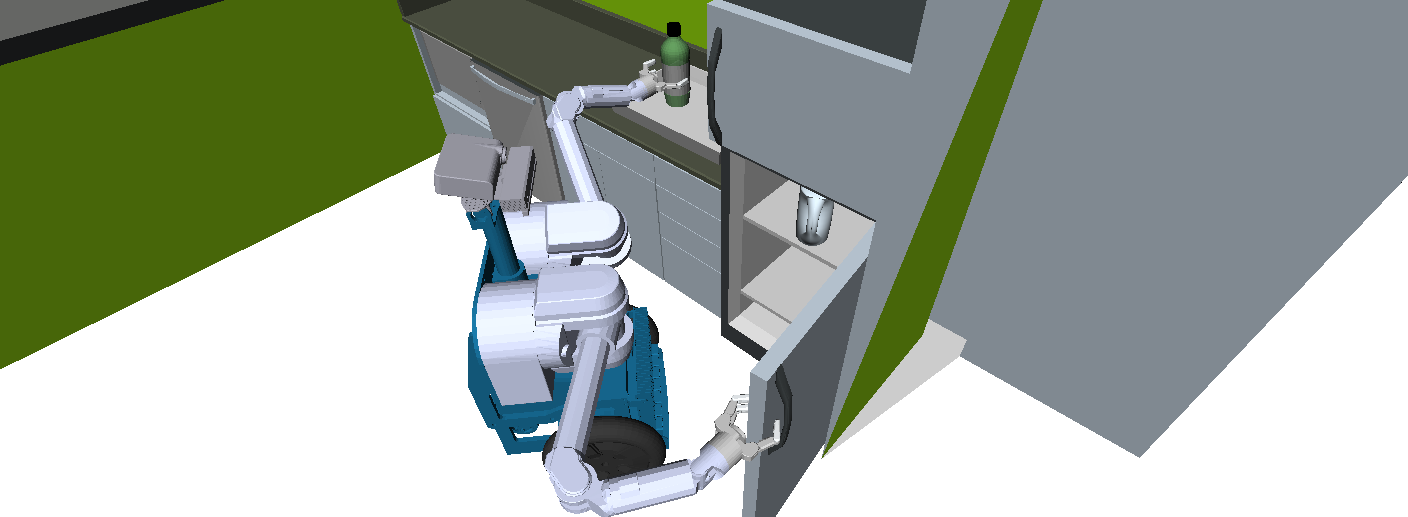
\includegraphics[width=11.5cm]{figs/herb-fridge-c.png}}%
      \only<5>{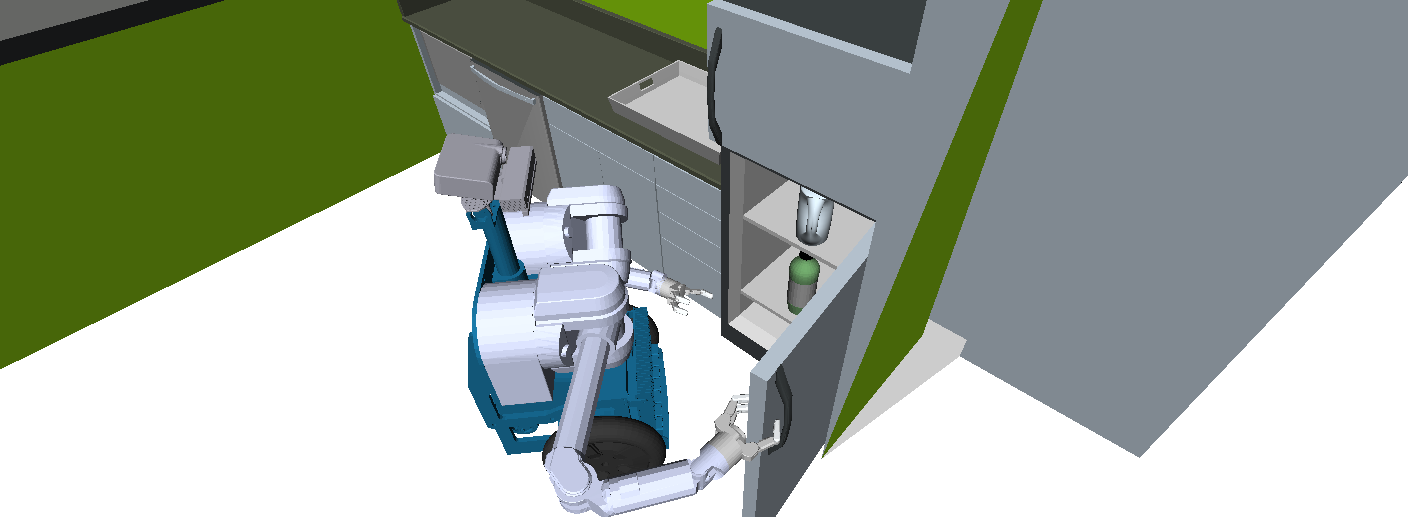
\includegraphics[width=11.5cm]{figs/herb-fridge-a.png}}%
   };

   % figure adapted from proposal doc
   \begin{scope}[font=\scriptsize,shift={(1.5,1.5)}]
      
      % root sets
      \only<3->{
         \node[draw,black,rounded corners,minimum height=1.5cm,minimum width=1cm]
            (Xgrasp) at (3,0) {};
         \node[above=0cm of Xgrasp] {Grasp};
      }
      \only<4->{
         \node[draw,black,rounded corners,minimum height=1.5cm,minimum width=1cm]
            (Xdrop) at (6,0) {};
         \node[above=0cm of Xdrop] {Place};
      }
      
      % nodes
      \only<2->
      {
         \node[circle,fill=black,inner sep=2] (xstart) at (0,0) {};
         \node[above=0.1cm of xstart] {$q_{\mbox{\scriptsize start}}$};
      }
      %\node[circle,fill=black,inner sep=2] (xg1) at (2.8,0.5) {};
      %\node[circle,fill=black,inner sep=2] (xg2) at (3.1,0.1) {};
      \only<3->{
         \node[circle,fill=black,inner sep=2] (xg3) at (2.9,-0.5) {};
      }
      \only<4->{
         \node[circle,fill=black,inner sep=2] (xd1) at (5.9,0.3) {};
      }
      %\node[circle,fill=black,inner sep=2] (xd2) at (6.0,-0.4) {};
      \only<5->
      {
         \node[circle,fill=black,inner sep=2] (xend) at (9,0) {};
         \node[above=0.1cm of xend] {$q_{\mbox{\scriptsize end}}$};
      }
      
      \only<3->{
         % in S1
         %\draw[line width=1.5mm,white]
         %   (xstart) .. controls (1,0.2) and (1.4,0.9) .. (xg1);
         %\draw[line width=1.5mm,white]
         %   (xstart) .. controls (1.5,0.2) .. (xg2);
         \draw[line width=1.5mm,white]
            (xstart) .. controls (1.8,-0.6) and (1.6,-0.8) .. (xg3);
         %\draw
         %   (xstart) .. controls (1,0.2) and (1.4,0.9) .. (xg1);
         %\draw
         %   (xstart) .. controls (1.5,0.2) .. (xg2);
         \draw
            (xstart) .. controls (1.8,-0.6) and (1.6,-0.8) .. (xg3);
      }
      
      \only<4->{
         % in s2
         %\draw[line width=1.5mm,white]
         %   (xg1) -- (4.7,0.6);
         %\draw[line width=1.5mm,white]
         %   (xg2) .. controls (4.5,1) and (3.5,-1.2) .. (4.5,-0.4)
         %         .. controls (5.5,0.5) and (5.0,-1.3) .. (xd2);
         %\draw
         %   (xg1) -- (4.7,0.6);
         %\draw
         %   (xg2) .. controls (4.5,1) and (3.5,-1.2) .. (4.5,-0.4)
         %         .. controls (5.5,0.5) and (5.0,-1.3) .. (xd2);
         \draw[line width=1.5mm,white]
            (xg3) .. controls (4.3, 0.2) and (4.5,-0.2) .. (xd1);
         \draw
            (xg3) .. controls (4.3, 0.2) and (4.5,-0.2) .. (xd1);
      }
      
      \only<5->{
         % in s3
         \draw[line width=1.5mm,white]
            (xd1) .. controls (8,0.3) and (8,0.1) .. (xend);
         \draw
            (xd1) .. controls (8,0.3) and (8,0.1) .. (xend);
      }
      
      \only<3->{
         \node[fill,black,rounded corners,minimum height=1.5cm,minimum width=1cm,
            opacity=0.1] at (3,0) {};
      }
      \only<4->{
         \node[fill,black,rounded corners,minimum height=1.5cm,minimum width=1cm,
            opacity=0.1] at (6,0) {};
      }
      
      %\draw [decorate,decoration={brace,mirror,amplitude=5pt}]
      %(0.0,-0.9) -- (2.9,-0.9) node [black,midway,yshift=-0.4cm,align=center]
      %   {bottle in fridge};

      %\draw [decorate,decoration={brace,mirror,amplitude=5pt}]
      %(3.1,-0.9) -- (5.9,-0.9) node [black,midway,yshift=-0.4cm,align=center]
      %   {bottle in hand};

      %\draw [decorate,decoration={brace,mirror,amplitude=5pt}]
      %(6.1,-0.9) -- (9.0,-0.9) node [black,midway,yshift=-0.4cm,align=center]
      %   {bottle on tray};
   \end{scope}

   %\node[inner sep=0pt] at (6,2.25) {
   %   \includegraphics{build/intro-subprob-cspace}
   %};
   
   %In order to describe why it's so slow,
   %I need to talk a bit about the problem's structure
   %and current approaches to handling it.
   %
   %I will be using this HERB example (removing items from a fridge)
   %throughout the talk.
   %
   %Below, show a 2D diagram of three steps of this plan,
   %which I then reference in the next three challenge slides.
   
   \end{tikzpicture}
\end{frame}

\begin{frame}
   \frametitle{Challenge 1: The Planning vs. Execution Tradeoff}
   \begin{tikzpicture}
      \draw[step=1,black!10,very thin,opacity=\gridopacity] (0,0) grid (12,8);

   \node[inner sep=0pt] at (3,5.3) {%
      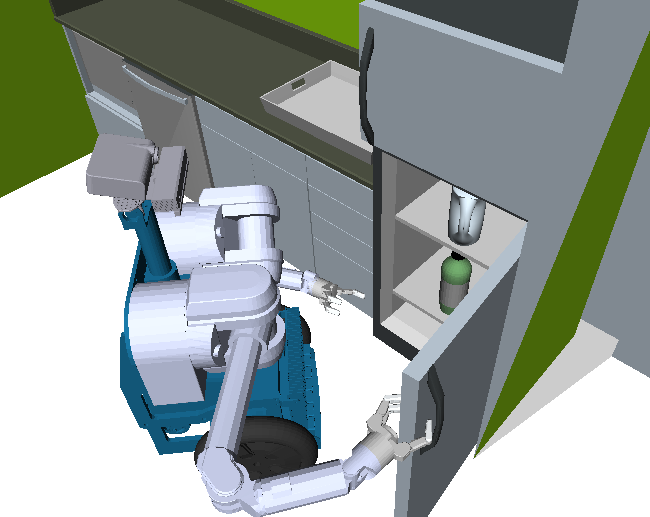
\includegraphics[width=5.75cm]{figs/herb-fridge-a-skinny.png}
   };

   \only<3->{
      \node[fill=black!5,rounded corners,font=\small,anchor=north] at (9,7.5)
         {\begin{minipage}{5.5cm}

            Configuration space $\mathcal{C}$ is:
            \only<4->{
               \begin{itemize}[leftmargin=*,itemsep=0pt,topsep=2pt]
               \item continuous
               \only<5->{\item high-dimensional}
               \end{itemize}
            }
         
            \only<7->{
               \medskip
               Valid subset $\mathcal{C}_{\ms{free}}$ is:
            }
            \only<8->{
               \begin{itemize}[leftmargin=*,itemsep=0pt,topsep=2pt]
               \item induced by complex geometry
               \only<9->{\item expensive to validate motions}
               \end{itemize}
            }
            
            \only<10->{
               \begin{center}
                  {\bf Planning is expensive!}
               \end{center}
            }
            
         \end{minipage}};
   }
   
   \only<11->{
      \node[fill=blue!10,rounded corners,font=\small,anchor=north] at (9,3)
         {\begin{minipage}{5.5cm}
            \begin{center}
            For manipulation tasks,\\
            planning effort $\approx$ execution effort
            \end{center}
         \end{minipage}};
   }
   
   \only<12->{
      \node[fill=blue!10,rounded corners,font=\small,anchor=north] at (9,1.75)
         {\begin{minipage}{5.5cm}
            \begin{center}
            Robot's effort spent planning
            detracts directly from available
            task resource budget.
            \end{center}
         \end{minipage}};
   }

   % figure adapted from proposal doc
   \begin{scope}[font=\scriptsize,shift={(1.5,1.5)}]
      
      % root sets
      \node[draw,black,rounded corners,minimum height=1.5cm,minimum width=1cm]
         (Xgrasp) at (3,0) {};
      \node[above=0cm of Xgrasp] {Grasp};
      
      % cspace sets (lines only)
      \only<2->{
         \node[draw,black,rounded corners,minimum height=1.8cm,minimum width=1.8cm,dashed]
            (S1) at (1.5,0) {};
         \node[above left=-0.7cm of S1] {$\mathcal{C}$};
      }
      
      % nodes
      \node[circle,fill=black,inner sep=2] (xstart) at (0,0) {};
      \node[above=0.1cm of xstart] {$q_{\mbox{\scriptsize start}}$};
      \node[circle,fill=black,inner sep=2] (xg3) at (2.9,-0.5) {};
      
      % in S1
      \draw[line width=1.5mm,white]
         (xstart) .. controls (1.8,-0.6) and (1.6,-0.8) .. (xg3);
      
      % draw s1 cfree
      \only<6->{
         \begin{scope}[even odd rule]
            \clip[rounded corners] (0.61,-0.89) rectangle (2.39,0.89);
            \clip[rotate around={10:(1.1,0.5)}] (-3,-3) rectangle (3,3)
                     (0.6,-0.0) rectangle (1.6,1.0);
            \fill[blue!15,rotate around={-15:(1.5,-0.5)}] (1.5,-0.5) ellipse (1.4cm and 0.5cm);
            \fill[blue!15,rotate around={-25:(1.5, 1.0)}] (1.5, 1.0) ellipse (1.4cm and 0.5cm);
         \end{scope}
         \node[draw,inner sep=0,fill=blue!20,minimum width=0.5cm,minimum height=0.2cm]
            (Cfreebox1) at (1.2, -1.2) {};
         \node[right=0cm of Cfreebox1] {: $\mathcal{C}_{\mbox{\tiny free}}$}; 
      }
         
      \draw
         (xstart) .. controls (1.8,-0.6) and (1.6,-0.8) .. (xg3);
      
      \node[fill,black,rounded corners,minimum height=1.5cm,minimum width=1cm,
         opacity=0.1] at (3,0) {};
      
      %\draw [decorate,decoration={brace,mirror,amplitude=5pt}]
      %(0.0,-0.9) -- (2.9,-0.9) node [black,midway,yshift=-0.4cm,align=center]
      %   {bottle in fridge};

      %\draw [decorate,decoration={brace,mirror,amplitude=5pt}]
      %(3.1,-0.9) -- (5.9,-0.9) node [black,midway,yshift=-0.4cm,align=center]
      %   {bottle in hand};

      %\draw [decorate,decoration={brace,mirror,amplitude=5pt}]
      %(6.1,-0.9) -- (9.0,-0.9) node [black,midway,yshift=-0.4cm,align=center]
      %   {bottle on tray};
   \end{scope}

   \end{tikzpicture}
\end{frame}

\begin{frame}
   \frametitle{Challenge 2: Incongruent Steps Impede Reuse}
   \begin{tikzpicture}
      \draw[step=1,black!10,very thin,opacity=\gridopacity] (0,0) grid (12,8);

   \node[inner sep=0pt] at (3,5.3) {%
      \only<1>{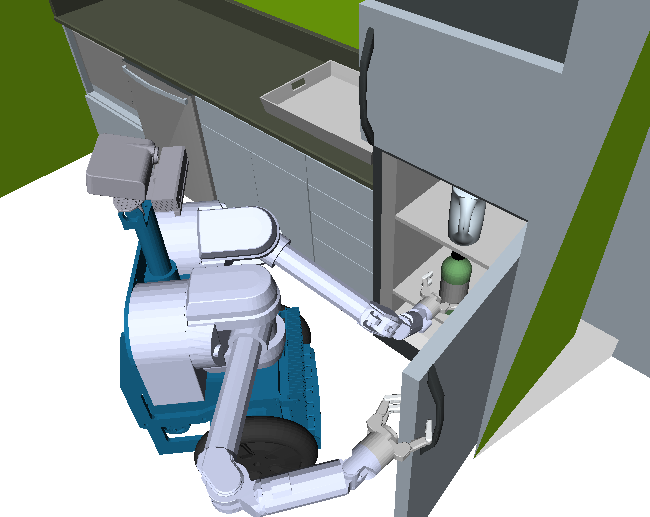
\includegraphics[width=5.75cm]{figs/herb-fridge-b-skinny.png}}%
      \only<2->{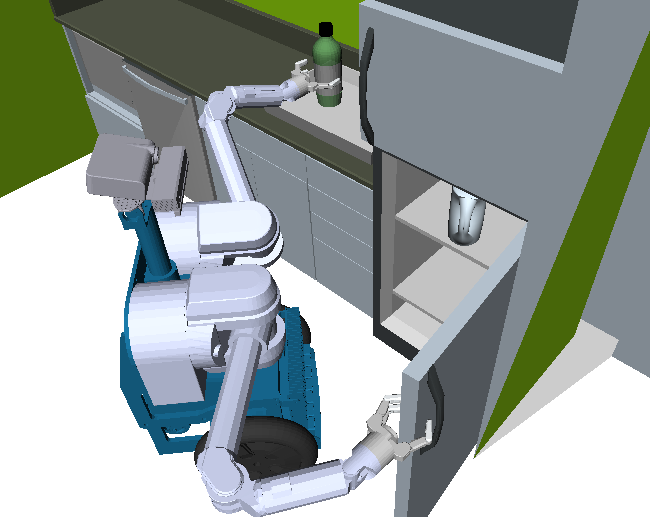
\includegraphics[width=5.75cm]{figs/herb-fridge-c-skinny.png}}%
   };

   \only<5->{
      \node[fill=black!5,rounded corners,font=\small,anchor=north] at (9,7.5)
         {\begin{minipage}{5.5cm}
            $\mathcal{C}_{\ms{free}}$ is dependent on:
            \begin{itemize}[leftmargin=*,itemsep=0pt,topsep=2pt]
               \item distribution of all obstacles
               \item grasp pose of held objects
               \item robot location
            \end{itemize}
         \end{minipage}};
   }
   
   \only<6->{
      \node[fill=blue!10,rounded corners,font=\small,anchor=north] at (9,5.3)
         {\begin{minipage}{5.5cm}
            \begin{center}
            For manipulation tasks,\\
            this subset changes at \emph{every} step!
            \end{center}
         \end{minipage}};
   }
   
   \only<7->{
      \node[fill=blue!10,rounded corners,font=\small,anchor=north] at (9,4.1)
         {\begin{minipage}{5.5cm}
            \begin{center}
            How can we reuse precious planning computation?
            \end{center}
         \end{minipage}};
   }

   % figure adapted from proposal doc
   \begin{scope}[font=\scriptsize,shift={(1.5,1.5)}]
      
      % root sets
      \node[draw,black,rounded corners,minimum height=1.5cm,minimum width=1cm]
         (Xgrasp) at (3,0) {};
      \node[above=0cm of Xgrasp] {Grasp};
      
      \only<3->{
         \node[draw,black,rounded corners,minimum height=1.5cm,minimum width=1cm]
            (Xdrop) at (6,0) {};
         \node[above=0cm of Xdrop] {Place};
      }
      
      % cspace sets
      \node[draw,black,rounded corners,minimum height=1.8cm,minimum width=1.8cm,dashed]
         (S1) at (1.5,0) {};
      \node[above left=-0.7cm of S1] {$\mathcal{C}$};
      
      \only<4->{
         \node[draw,black,rounded corners,minimum height=1.8cm,minimum width=1.8cm,dashed]
            (S1) at (4.5,0) {};
         \node[above left=-0.7cm of S1] {$\mathcal{C}$};
      }
      
      % nodes
      \node[circle,fill=black,inner sep=2] (xstart) at (0,0) {};
      \node[above=0.1cm of xstart] {$q_{\mbox{\scriptsize start}}$};
      \node[circle,fill=black,inner sep=2] (xg3) at (2.9,-0.5) {};
      
      % in S1
      \draw[line width=1.5mm,white]
         (xstart) .. controls (1.8,-0.6) and (1.6,-0.8) .. (xg3);
      % draw s1 cfree
      \begin{scope}[even odd rule]
         \clip[rounded corners] (0.61,-0.89) rectangle (2.39,0.89);
         \clip[rotate around={10:(1.1,0.5)}] (-3,-3) rectangle (3,3)
                  (0.6,-0.0) rectangle (1.6,1.0);
         \fill[blue!15,rotate around={-15:(1.5,-0.5)}] (1.5,-0.5) ellipse (1.4cm and 0.5cm);
         \fill[blue!15,rotate around={-25:(1.5, 1.0)}] (1.5, 1.0) ellipse (1.4cm and 0.5cm);
      \end{scope}
      \node[draw,inner sep=0,fill=blue!20,minimum width=0.5cm,minimum height=0.2cm]
            (Cfreebox1) at (1.2, -1.2) {};
         \node[right=0cm of Cfreebox1] {: $\mathcal{C}_{\mbox{\tiny free1}}$}; 
      \draw
         (xstart) .. controls (1.8,-0.6) and (1.6,-0.8) .. (xg3);
      
      % in s2
      \only<3->{
         \node[circle,fill=black,inner sep=2] (xd1) at (5.9,0.3) {};
         \draw[line width=1.5mm,white]
            (xg3) .. controls (4.3, 0.2) and (4.5,-0.2) .. (xd1);
         \only<4->{
            % draw s2 cfree
            \begin{scope}[even odd rule]
               \clip[rounded corners] (3.61,-0.89) rectangle (5.39,0.89);
               \clip[rotate around={10:(4.1,0.5)}] (0,-3) rectangle (6,3)
                     (3.6,-0.0) rectangle (4.6,1.0);
               \fill[red!15,rotate around={15:(4.5,-0.2)}] (4.5,-0.2) ellipse (1.4cm and 0.5cm);
            \end{scope}
            \node[draw,inner sep=0,fill=red!20,minimum width=0.5cm,minimum height=0.2cm]
               (Cfreebox1) at (4.2, -1.2) {};
            \node[right=0cm of Cfreebox1] {: $\mathcal{C}_{\mbox{\tiny free2}}$};
         }
         \draw
            (xg3) .. controls (4.3, 0.2) and (4.5,-0.2) .. (xd1);
      }
      
      \node[fill,black,rounded corners,minimum height=1.5cm,minimum width=1cm,
         opacity=0.1] at (3,0) {};
      \only<3->{
         \node[fill,black,rounded corners,minimum height=1.5cm,minimum width=1cm,
            opacity=0.1] at (6,0) {};
      }
      
      %\draw [decorate,decoration={brace,mirror,amplitude=5pt}]
      %(0.0,-0.9) -- (2.9,-0.9) node [black,midway,yshift=-0.4cm,align=center]
      %   {bottle in fridge};

      %\draw [decorate,decoration={brace,mirror,amplitude=5pt}]
      %(3.1,-0.9) -- (5.9,-0.9) node [black,midway,yshift=-0.4cm,align=center]
      %   {bottle in hand};

      %\draw [decorate,decoration={brace,mirror,amplitude=5pt}]
      %(6.1,-0.9) -- (9.0,-0.9) node [black,midway,yshift=-0.4cm,align=center]
      %   {bottle on tray};
   \end{scope}

   \end{tikzpicture}
\end{frame}

\begin{frame}
   \frametitle{Challenge 3: Coupled Steps Require Planning Ahead}
   \begin{tikzpicture}
      \draw[step=1,black!10,very thin,opacity=\gridopacity] (0,0) grid (12,8);

   \node[inner sep=0pt] at (3,5.3) {%
      \only<1->{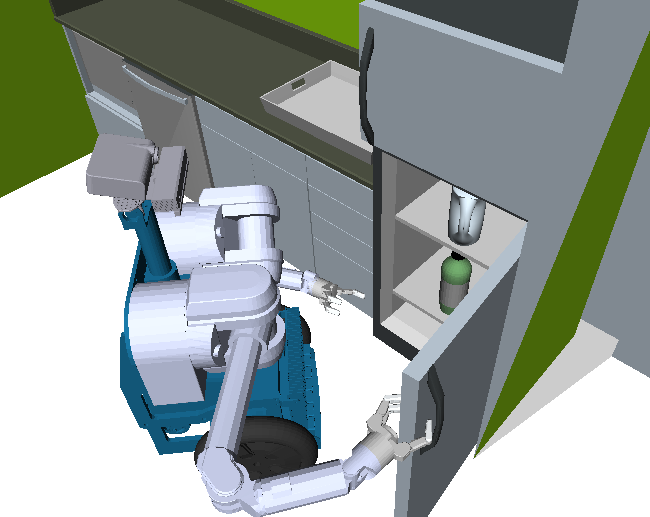
\includegraphics[width=5.75cm]{figs/herb-fridge-a-skinny.png}}%
      %\only<2->{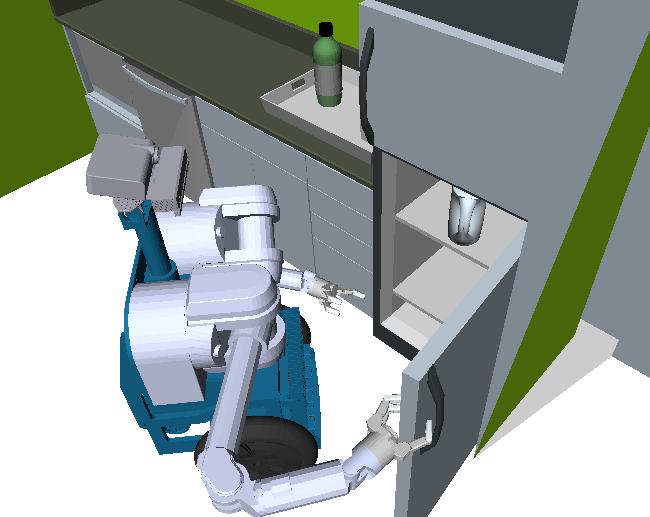
\includegraphics[width=5.75cm]{figs/herb-fridge-d-skinny.png}}%
   };

   \only<2->{
      \node[fill=black!5,rounded corners,font=\small,anchor=north] at (9,7.7)
         {\begin{minipage}{5.5cm}
            Each step admits several choices:
            \begin{itemize}[leftmargin=*,itemsep=0pt,topsep=2pt]
               \item which object
               \item which grasp/placement
               \item which IK solution
            \end{itemize}
         \end{minipage}};
   }
   
   \only<3->{
      \node[fill=blue!10,rounded corners,font=\small,anchor=north] at (9,5.5)
         {\begin{minipage}{5.5cm}
            \begin{center}
            For manipulation tasks,\\
            a bad choice can render ensuing steps \emph{impossible}
            \only<-4>{\color{blue!10}or \emph{difficult}.}%
            \only<5->{or \emph{difficult}.}%
            \end{center}
         \end{minipage}};
   }
   
   \only<10->{
      \node[fill=blue!10,rounded corners,font=\small,anchor=north] at (9,3.9)
         {\begin{minipage}{5.5cm}
            \begin{center}
            This magnifies the need for efficient motion planning.
            \end{center}
         \end{minipage}};
   }

   % figure adapted from proposal doc
   \begin{scope}[font=\scriptsize,shift={(1.5,1.5)}]
      
      % root sets
      \node[draw,black,rounded corners,minimum height=1.5cm,minimum width=1cm]
         (Xgrasp) at (3,0) {};
      \node[above=0cm of Xgrasp] {Grasp};
      \node[draw,black,rounded corners,minimum height=1.5cm,minimum width=1cm]
         (Xdrop) at (6,0) {};
      \node[above=0cm of Xdrop] {Place};
      
      % nodes
      \node[circle,fill=black,inner sep=2] (xstart) at (0,0) {};
      \node[above=0.1cm of xstart] {$q_{\mbox{\scriptsize start}}$};
      
      \only<2->{
         % grasp choices
         \node[circle,fill=black,inner sep=2] (xg1) at (2.8,0.5) {};
         \node[circle,fill=black,inner sep=2] (xg2) at (3.1,0.1) {};
         \node[circle,fill=black,inner sep=2] (xg3) at (2.9,-0.5) {};
         % place choices
         \node[circle,fill=black,inner sep=2] (xd1) at (5.9,0.3) {};
         \node[circle,fill=black,inner sep=2] (xd2) at (6.0,-0.4) {};
         % xend 
         \node[circle,fill=black,inner sep=2] (xend) at (9,0) {};
         \node[above=0.1cm of xend] {$q_{\mbox{\scriptsize end}}$};
      }
      
      %\only<2->{
      %   
      %}
      
      % in S1
      \only<3->{
         \draw[line width=1.5mm,white]
            (xstart) .. controls (1,0.2) and (1.4,0.9) .. (xg1);
      }
      \only<5->{
         \draw[line width=1.5mm,white]
            (xstart) .. controls (1.5,0.2) .. (xg2);
      }
      \only<7->{
         \draw[line width=1.5mm,white]
            (xstart) .. controls (1.8,-0.6) and (1.6,-0.8) .. (xg3);
      }
      \only<3->{
         \draw
            (xstart) .. controls (1,0.2) and (1.4,0.9) .. (xg1);
      }
      \only<5->{
         \draw
            (xstart) .. controls (1.5,0.2) .. (xg2);
      }
      \only<7->{
         \draw
            (xstart) .. controls (1.8,-0.6) and (1.6,-0.8) .. (xg3);
      }
      
      % in s2
      \only<4->{
         \draw[line width=1.5mm,white]
            (xg1) -- (4.7,0.6);
         \draw
            (xg1) -- (4.7,0.6);
      }
      \only<6->{
         \draw[line width=1.5mm,white]
            (xg2) .. controls (4.5,1) and (3.5,-1.2) .. (4.5,-0.4)
                  .. controls (5.5,0.5) and (5.0,-1.3) .. (xd2);
         \draw
            (xg2) .. controls (4.5,1) and (3.5,-1.2) .. (4.5,-0.4)
                  .. controls (5.5,0.5) and (5.0,-1.3) .. (xd2);
      }
      
      \only<8->{
         \draw[line width=1.5mm,white]
            (xg3) .. controls (4.3, 0.2) and (4.5,-0.2) .. (xd1);
         \draw
            (xg3) .. controls (4.3, 0.2) and (4.5,-0.2) .. (xd1);
      }
      
      \only<9->{
         % in s3
         \draw[line width=1.5mm,white]
            (xd1) .. controls (8,0.3) and (8,0.1) .. (xend);
         \draw
            (xd1) .. controls (8,0.3) and (8,0.1) .. (xend);
      }
      
      \node[fill,black,rounded corners,minimum height=1.5cm,minimum width=1cm,
         opacity=0.1] at (3,0) {};
      \node[fill,black,rounded corners,minimum height=1.5cm,minimum width=1cm,
         opacity=0.1] at (6,0) {};
      
   \end{scope}

   \end{tikzpicture}
\end{frame}

\begin{frame}
   \frametitle{Objective of Proposed Work}
   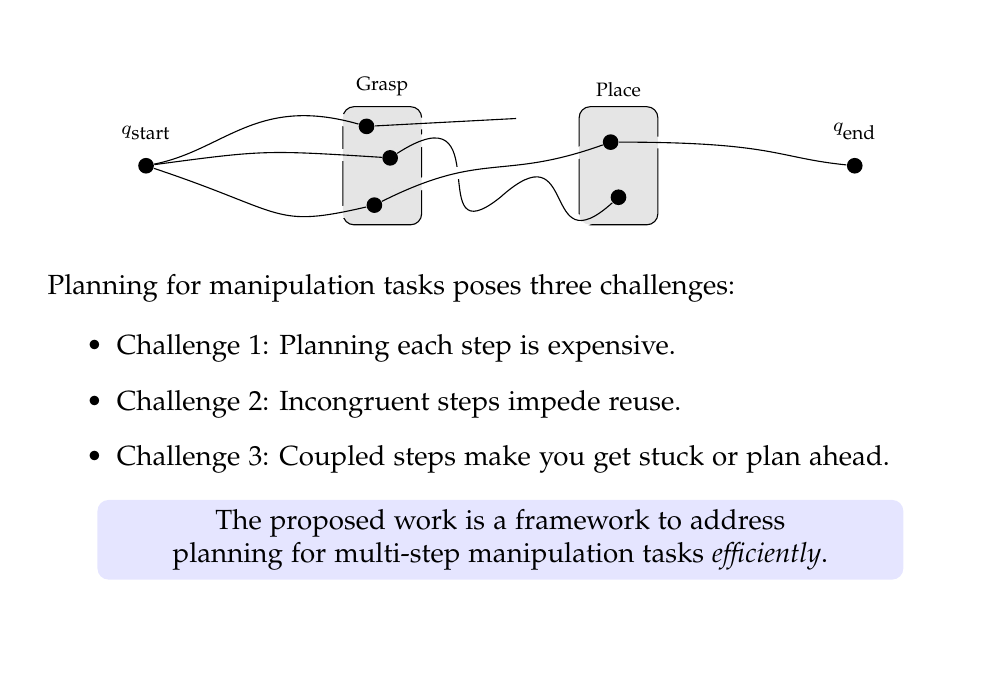
\begin{tikzpicture}
      \draw[step=1,black!10,very thin,opacity=\gridopacity] (0,0) grid (12,8);
   
      % figure adapted from proposal doc
      \begin{scope}[font=\scriptsize,shift={(1.5,6.25)}]
         
         % root sets
         \node[draw,black,rounded corners,minimum height=1.5cm,minimum width=1cm]
            (Xgrasp) at (3,0) {};
         \node[above=0cm of Xgrasp] {Grasp};
         \node[draw,black,rounded corners,minimum height=1.5cm,minimum width=1cm]
            (Xdrop) at (6,0) {};
         \node[above=0cm of Xdrop] {Place};
         
         % nodes
         \node[circle,fill=black,inner sep=2] (xstart) at (0,0) {};
         \node[above=0.1cm of xstart] {$q_{\mbox{\scriptsize start}}$};
         
         % grasp choices
         \node[circle,fill=black,inner sep=2] (xg1) at (2.8,0.5) {};
         \node[circle,fill=black,inner sep=2] (xg2) at (3.1,0.1) {};
         \node[circle,fill=black,inner sep=2] (xg3) at (2.9,-0.5) {};
         % place choices
         \node[circle,fill=black,inner sep=2] (xd1) at (5.9,0.3) {};
         \node[circle,fill=black,inner sep=2] (xd2) at (6.0,-0.4) {};
         % xend 
         \node[circle,fill=black,inner sep=2] (xend) at (9,0) {};
         \node[above=0.1cm of xend] {$q_{\mbox{\scriptsize end}}$};
         
         \draw[line width=1.5mm,white]
            (xstart) .. controls (1,0.2) and (1.4,0.9) .. (xg1);
         \draw[line width=1.5mm,white]
            (xstart) .. controls (1.5,0.2) .. (xg2);
         \draw[line width=1.5mm,white]
            (xstart) .. controls (1.8,-0.6) and (1.6,-0.8) .. (xg3);
         \draw
            (xstart) .. controls (1,0.2) and (1.4,0.9) .. (xg1);
         \draw
            (xstart) .. controls (1.5,0.2) .. (xg2);
         \draw
            (xstart) .. controls (1.8,-0.6) and (1.6,-0.8) .. (xg3);
         \draw[line width=1.5mm,white]
            (xg1) -- (4.7,0.6);
         \draw
            (xg1) -- (4.7,0.6);
         \draw[line width=1.5mm,white]
            (xg2) .. controls (4.5,1) and (3.5,-1.2) .. (4.5,-0.4)
                  .. controls (5.5,0.5) and (5.0,-1.3) .. (xd2);
         \draw
            (xg2) .. controls (4.5,1) and (3.5,-1.2) .. (4.5,-0.4)
                  .. controls (5.5,0.5) and (5.0,-1.3) .. (xd2);
         \draw[line width=1.5mm,white]
            (xg3) .. controls (4.3, 0.2) and (4.5,-0.2) .. (xd1);
         \draw
            (xg3) .. controls (4.3, 0.2) and (4.5,-0.2) .. (xd1);
         % in s3
         \draw[line width=1.5mm,white]
            (xd1) .. controls (8,0.3) and (8,0.1) .. (xend);
         \draw
            (xd1) .. controls (8,0.3) and (8,0.1) .. (xend);
         
         \node[fill,black,rounded corners,minimum height=1.5cm,minimum width=1cm,
            opacity=0.1] at (3,0) {};
         \node[fill,black,rounded corners,minimum height=1.5cm,minimum width=1cm,
            opacity=0.1] at (6,0) {};
         
      \end{scope}
   
   
      \node[anchor=north] at (6,5) {\begin{minipage}{11.5cm}
         Planning for manipulation tasks poses three challenges:
         
         \begin{itemize}
         \item Challenge 1: Planning each step is expensive.
         \item Challenge 2: Incongruent steps impede reuse.
         \item Challenge 3: Coupled steps make you get stuck or plan ahead.
         \end{itemize}
      \end{minipage}};
   
      \node[fill=blue!10,rounded corners] at (6,1.5) {\begin{minipage}{10cm}\centering
         The proposed work is a framework to address\\
         planning for multi-step manipulation tasks \emph{efficiently}.
      \end{minipage}};
   
   \end{tikzpicture}
\end{frame}


\begin{frame}
   \frametitle{Part 1: Capturing the Planning/Execution Tradeoff}
      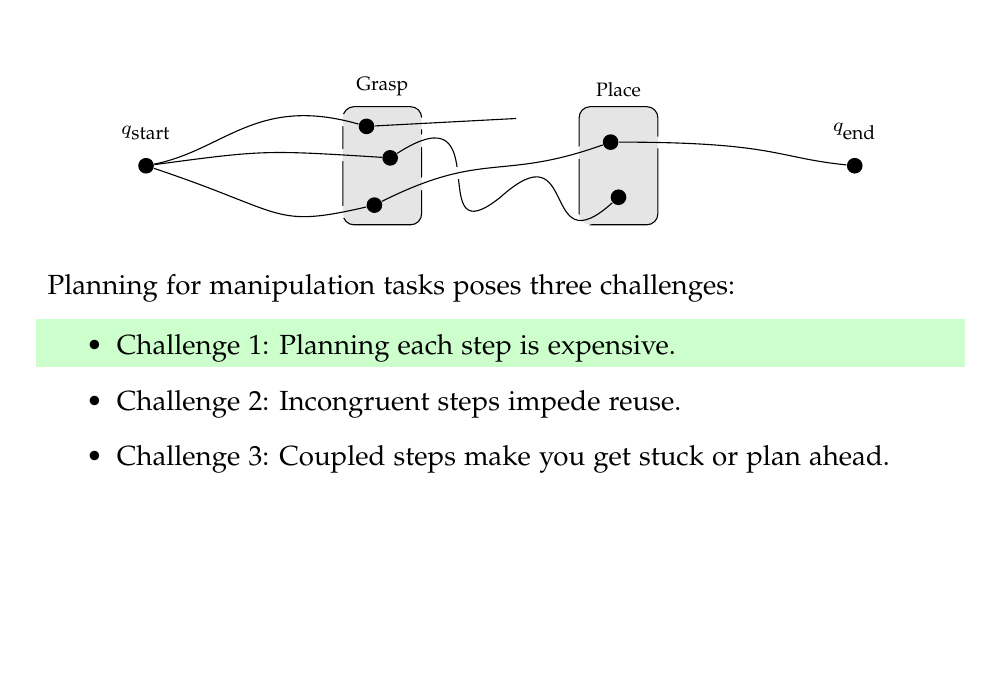
\begin{tikzpicture}
      \draw[step=1,black!10,very thin,opacity=\gridopacity] (0,0) grid (12,8);
   
      % figure adapted from proposal doc
      \begin{scope}[font=\scriptsize,shift={(1.5,6.25)}]
         
         % root sets
         \node[draw,black,rounded corners,minimum height=1.5cm,minimum width=1cm]
            (Xgrasp) at (3,0) {};
         \node[above=0cm of Xgrasp] {Grasp};
         \node[draw,black,rounded corners,minimum height=1.5cm,minimum width=1cm]
            (Xdrop) at (6,0) {};
         \node[above=0cm of Xdrop] {Place};
         
         % nodes
         \node[circle,fill=black,inner sep=2] (xstart) at (0,0) {};
         \node[above=0.1cm of xstart] {$q_{\mbox{\scriptsize start}}$};
         
         % grasp choices
         \node[circle,fill=black,inner sep=2] (xg1) at (2.8,0.5) {};
         \node[circle,fill=black,inner sep=2] (xg2) at (3.1,0.1) {};
         \node[circle,fill=black,inner sep=2] (xg3) at (2.9,-0.5) {};
         % place choices
         \node[circle,fill=black,inner sep=2] (xd1) at (5.9,0.3) {};
         \node[circle,fill=black,inner sep=2] (xd2) at (6.0,-0.4) {};
         % xend 
         \node[circle,fill=black,inner sep=2] (xend) at (9,0) {};
         \node[above=0.1cm of xend] {$q_{\mbox{\scriptsize end}}$};
         
         \draw[line width=1.5mm,white]
            (xstart) .. controls (1,0.2) and (1.4,0.9) .. (xg1);
         \draw[line width=1.5mm,white]
            (xstart) .. controls (1.5,0.2) .. (xg2);
         \draw[line width=1.5mm,white]
            (xstart) .. controls (1.8,-0.6) and (1.6,-0.8) .. (xg3);
         \draw
            (xstart) .. controls (1,0.2) and (1.4,0.9) .. (xg1);
         \draw
            (xstart) .. controls (1.5,0.2) .. (xg2);
         \draw
            (xstart) .. controls (1.8,-0.6) and (1.6,-0.8) .. (xg3);
         \draw[line width=1.5mm,white]
            (xg1) -- (4.7,0.6);
         \draw
            (xg1) -- (4.7,0.6);
         \draw[line width=1.5mm,white]
            (xg2) .. controls (4.5,1) and (3.5,-1.2) .. (4.5,-0.4)
                  .. controls (5.5,0.5) and (5.0,-1.3) .. (xd2);
         \draw
            (xg2) .. controls (4.5,1) and (3.5,-1.2) .. (4.5,-0.4)
                  .. controls (5.5,0.5) and (5.0,-1.3) .. (xd2);
         \draw[line width=1.5mm,white]
            (xg3) .. controls (4.3, 0.2) and (4.5,-0.2) .. (xd1);
         \draw
            (xg3) .. controls (4.3, 0.2) and (4.5,-0.2) .. (xd1);
         % in s3
         \draw[line width=1.5mm,white]
            (xd1) .. controls (8,0.3) and (8,0.1) .. (xend);
         \draw
            (xd1) .. controls (8,0.3) and (8,0.1) .. (xend);
         
         \node[fill,black,rounded corners,minimum height=1.5cm,minimum width=1cm,
            opacity=0.1] at (3,0) {};
         \node[fill,black,rounded corners,minimum height=1.5cm,minimum width=1cm,
            opacity=0.1] at (6,0) {};
         
      \end{scope}
   
      \fill[green!20] (0.1,3.7) rectangle (11.9,4.3);
   
      \node[anchor=north] at (6,5) {\begin{minipage}{11.5cm}
         Planning for manipulation tasks poses three challenges:
         
         \begin{itemize}
         \item Challenge 1: Planning each step is expensive.
         \item Challenge 2: Incongruent steps impede reuse.
         \item Challenge 3: Coupled steps make you get stuck or plan ahead.
         \end{itemize}
      \end{minipage}};
   
   \end{tikzpicture}
\end{frame}
   
\begin{frame}
   \frametitle{Motion Planning in Configuration Space}
   \begin{tikzpicture}
      \draw[step=1,black!10,very thin,opacity=\gridopacity] (0,0) grid (12,8);
      
      \node[inner sep=0] at (3,4)
         {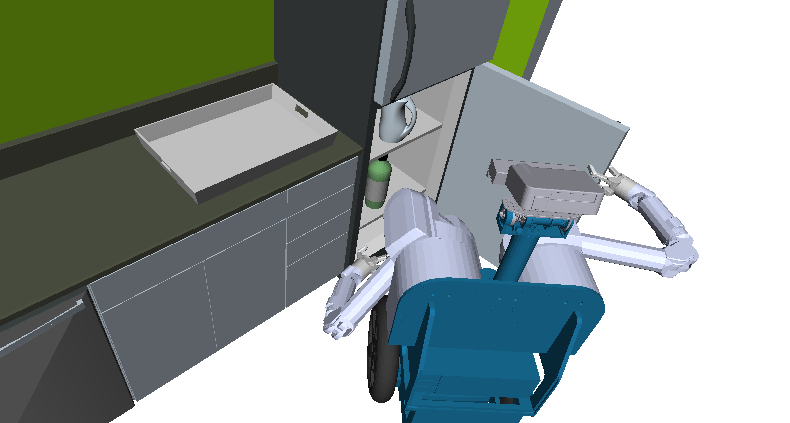
\includegraphics[width=5cm]{figs/fridge-intro.png}};
   
      \node[inner sep=0] at (9,5) {%
         {\only<1>{\includegraphics{build/talk-act1-2d,rootsonly}}}%
         {\only<2>{\includegraphics{build/talk-act1-2d,cfree}}}%
         {\only<3>{\includegraphics{build/talk-act1-2d,paths}}}%
      };
      
      % legend
      \only<2->{
         \node[draw,line width=1.5pt,fill=blue!20,minimum width=0.75cm,minimum height=0.10cm]
            (Cfreebox) at (3.0, 7.0) {};
         \node[right=0cm of Cfreebox] {: $\mathcal{C}_{\mbox{\scriptsize free}}$}; 
      }
      \only<3->{
         \node at (3,6.25) {$\Pi$ : set of candidate paths};
      }
      
      \only<1>{\node at (6,1) {High-dimensional C-space (cite TLP).};}
      \only<2>{\node at (6,1.3) {\begin{minipage}{11cm}\begin{center}
         \begin{equation*}
            f_x(\pi) = x(\pi)
         \end{equation*}
         Lots of possible paths.

         {\bf How to find low-cost paths quickly?}%
         \end{center}\end{minipage}
      };}
      \only<3>{\node at (6,1.3) {\begin{minipage}{11cm}\begin{center}
         \begin{equation*}
            f_x(\pi) =
            \left\{ \begin{array}{ll}
                x(\pi) & \mbox{if } {\bf 1}_{\mbox{\scriptsize free}}(\pi) \\
                \infty & \mbox{otherwise}
            \end{array} \right.
         \end{equation*}
         
         It has an indicator function,
         which is expensive to evaluate.
         \end{center}\end{minipage}
      };}
   
   \end{tikzpicture}
\end{frame}

\begin{frame}
   \frametitle{Best-First Search over Paths}
   \begin{tikzpicture}
   
      \draw[step=1,black!10,very thin,opacity=\gridopacity] (0,0) grid (12,8);
      
      \node[inner sep=0] at (9,5) {%
         {\only<1>{\includegraphics{build/talk-act1-2d,paths}}}%
         {\only<2>{\includegraphics{build/talk-act1-2d,traja}}}%
         {\only<3>{\includegraphics{build/talk-act1-2d,firstfail}}}%
         {\only<4>{\includegraphics{build/talk-act1-2d,firstfailnext}}}%
      };
      
      % legend
      \node[draw,line width=1.5pt,fill=blue!20,minimum width=0.75cm,minimum height=0.10cm]
         (Cfreebox) at (3.0, 7.0) {};
      \node[right=0cm of Cfreebox] {: $\mathcal{C}_{\mbox{\scriptsize free}}$}; 
      \node at (3,6.25) {$\Pi$ : set of candidate paths};
      
      \only<1>{\fill[green!30] (0.5,4.1) rectangle (5.5,4.65);}
      \only<2>{\fill[green!30] (0.5,3.4) rectangle (5.5,4.1);}
      \only<3>{\fill[green!30] (0.5,2.9) rectangle (5.5,3.4);}
      \only<4>{\fill[green!30] (0.5,3.4) rectangle (5.5,4.65);}
      
      % bfs
      \node at (3,4) {\begin{minipage}{5cm}
         \begin{algorithmic}
         \Loop%
            \State $\Pi \leftarrow $ \textsc{GetPaths}$()$
            \State $\pi^* \leftarrow \argmin\limits_{\pi \in \Pi} f(\pi)$
            \State \textsc{EvalPath}$(\pi^*)$
         \EndLoop
         \end{algorithmic}
         \end{minipage}
      };
      
      %\only<2>{\node at (6,1) {Select best candidate path.};}
      %\only<3>{\node at (6,1) {Evaluate.};}
   
   \end{tikzpicture}
\end{frame}

\begin{frame}
   \frametitle{Best-First Search over Paths: RRTs}
   \begin{tikzpicture}
   
      \draw[step=1,black!10,very thin,opacity=\gridopacity] (0,0) grid (12,8);
      
      \node[inner sep=0] at (9,5) {%
         {\only<1>{\includegraphics{build/talk-act1-2d,rrtstart}}}%
         {\only<2>{\includegraphics{build/talk-act1-2d,rrtsample}}}%
         {\only<3>{\includegraphics{build/talk-act1-2d,rrtcandidates}}}%
      };
      
      % legend
      \node[draw,line width=1.5pt,fill=blue!20,minimum width=0.75cm,minimum height=0.10cm]
         (Cfreebox) at (3.0, 7.0) {};
      \node[right=0cm of Cfreebox] {: $\mathcal{C}_{\mbox{\scriptsize free}}$}; 
      \node at (3,6.25) {$\Pi$ : set of candidate paths};
      
      \only<3>{\fill[green!30] (0.5,4.1) rectangle (5.5,4.65);}
      
      % bfs
      \node at (3,4) {\begin{minipage}{5cm}
         \begin{algorithmic}
         \Loop%
            \State $\Pi \leftarrow $ \textsc{GetPaths}$()$
            \State $\pi^* \leftarrow \argmin\limits_{\pi \in \Pi} f(\pi)$
            \State \textsc{EvalPath}$(\pi^*)$
         \EndLoop
         \end{algorithmic}
         \end{minipage}
      };
      
      %\only<2>{\node at (6,1) {Select best candidate path.};}
      %\only<3>{\node at (6,1) {Evaluate.};}
   
   \end{tikzpicture}
\end{frame}

\begin{frame}
   \frametitle{Best-First Search over Paths}
   \begin{tikzpicture}
   
      \draw[step=1,black!10,very thin,opacity=\gridopacity] (0,0) grid (12,8);
      
      \node[inner sep=0] at (9,5) {%
         {\only<1>{\includegraphics{build/talk-act1-2d,firstfailnext}}}%
      };
      
      % legend
      \node[draw,line width=1.5pt,fill=blue!20,minimum width=0.75cm,minimum height=0.10cm]
         (Cfreebox) at (3.0, 7.0) {};
      \node[right=0cm of Cfreebox] {: $\mathcal{C}_{\mbox{\scriptsize free}}$}; 
      \node at (3,6.25) {$\Pi$ : set of candidate paths};
      
      \only<1>{\fill[green!30] (0.5,3.4) rectangle (5.5,4.65);}
      
      % bfs
      \node at (3,4) {\begin{minipage}{5cm}
         \begin{algorithmic}
         \Loop%
            \State $\Pi \leftarrow $ \textsc{GetPaths}$()$
            \State $\pi^* \leftarrow \argmin\limits_{\pi \in \Pi} f(\pi)$
            \State \textsc{EvalPath}$(\pi^*)$
         \EndLoop
         \end{algorithmic}
         \end{minipage}
      };
      
   \end{tikzpicture}
\end{frame}

\begin{frame}
   \frametitle{Best-First Search over Paths: Roadmaps}
   \begin{tikzpicture}
   
      \draw[step=1,black!10,very thin,opacity=\gridopacity] (0,0) grid (12,8);
      
      \node[inner sep=0] at (9,5) {%
         {\only<1>{\includegraphics{build/talk-act1-2d,graph}}}%
         {\only<2>{\includegraphics{build/talk-act1-2d,graphfirst}}}%
         {\only<3>{\includegraphics{build/talk-act1-2d,graphfirstevaled}}}%
         {\only<4>{\includegraphics{build/talk-act1-2d,graphfirstnext}}}%
         {\only<5>{\includegraphics{build/talk-act1-2d,graph}}}%
         {\only<6>{\includegraphics{build/talk-act1-2d,astara}}}%
      };
      
      % legend
      \node[draw,line width=1.5pt,fill=blue!20,minimum width=0.75cm,minimum height=0.10cm]
         (Cfreebox) at (3.0, 7.0) {};
      \node[right=0cm of Cfreebox] {: $\mathcal{C}_{\mbox{\scriptsize free}}$}; 
      \node at (3,6.25) {$\Pi$ : set of candidate paths};
      
      \only<1>{\fill[green!30] (0.5,4.1) rectangle (5.5,4.65);}
      \only<2>{\fill[green!30] (0.5,3.4) rectangle (5.5,4.1);}
      \only<3>{\fill[green!30] (0.5,2.9) rectangle (5.5,3.4);}
      \only<4>{\fill[green!30] (0.5,3.4) rectangle (5.5,4.1);}
      
      % bfs
      \node at (3,4) {\begin{minipage}{5cm}
         \begin{algorithmic}
         \Loop%
            \State $\Pi \leftarrow $ \textsc{GetPaths}$()$
            \State $\pi^* \leftarrow \argmin\limits_{\pi \in \Pi} f(\pi)$
            \State \textsc{EvalPath}$(\pi^*)$
         \EndLoop
         \end{algorithmic}
         \end{minipage}
      };
      
      \only<1-4>{
         \node at (6,1) {E.g. Probabalistic RoadMap, state lattice, etc.};
      }
      
   \end{tikzpicture}
\end{frame}

\begin{frame}
   \frametitle{Graph Search}
   \begin{tikzpicture}
   
      \draw[step=1,black!10,very thin,opacity=\gridopacity] (0,0) grid (12,8);
      
      % example (FIRST) problems
      \only<4-14>
      {
         \node[inner sep=0pt] at (6.5,7) {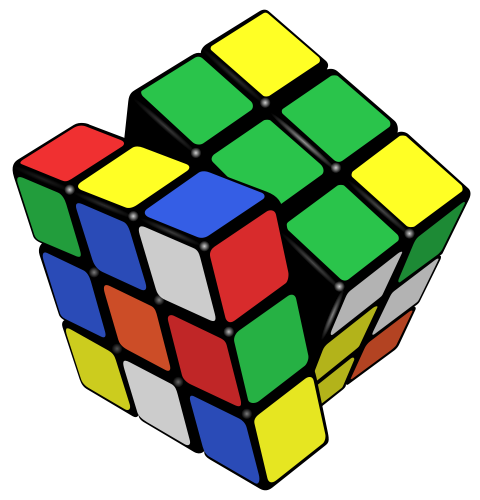
\includegraphics[width=1.5cm]{figs/rubik.png}};
         \node[inner sep=0pt,anchor=north,align=center,font=\scriptsize] at (6.5,6) {$4.3 \times 10^{19}$\\vertices};
      }
      
      \only<5-14>
      {
         \node[inner sep=0pt] at (8.5,7) {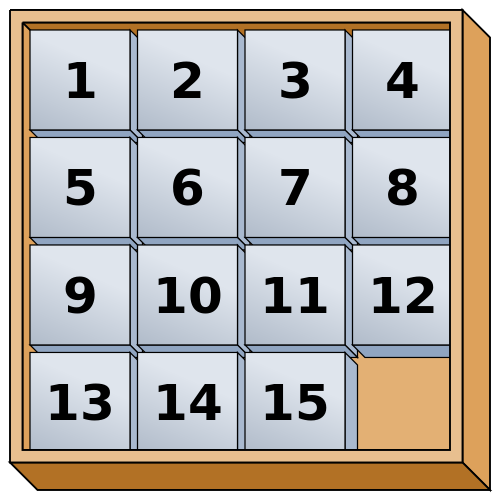
\includegraphics[width=1.5cm]{figs/15puzzle.png}};
         \node[inner sep=0pt,anchor=north,align=center,font=\scriptsize] at (8.5,6) {$2.1 \times 10^{13}$\\vertices};
      }
      
      \only<6-14>
      {
         \node[inner sep=0pt] at (10.5,7) {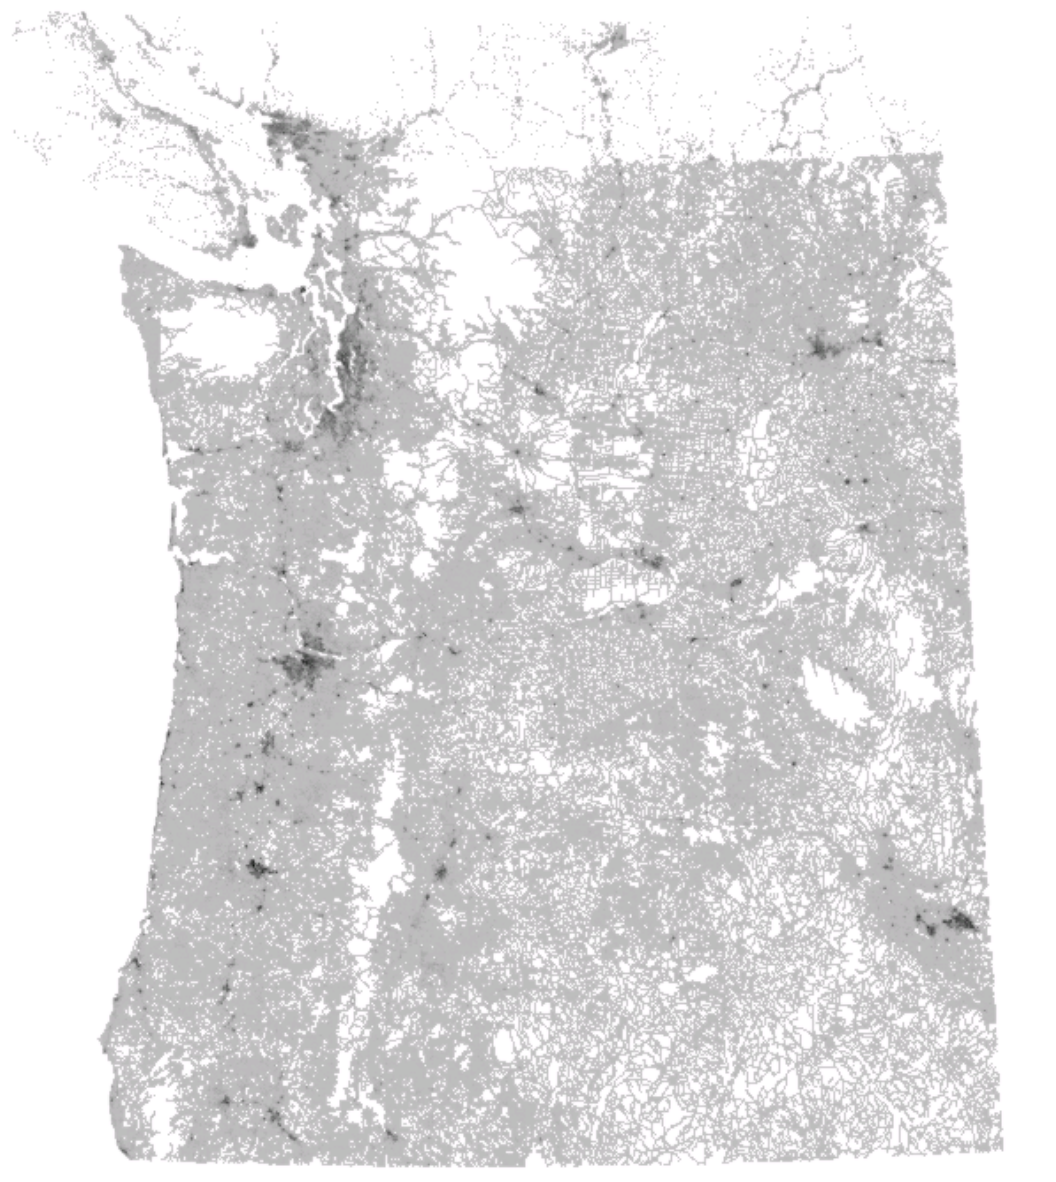
\includegraphics[width=1.5cm]{figs/goldberg-northwest.png}};
         \node[inner sep=0pt,anchor=north,align=center,font=\scriptsize] at (10.5,6) {1.6M\\vertices};
      }
      
      % example problems SECOND
      \only<17->
      {
         \node[inner sep=0pt] at (2.0,7) {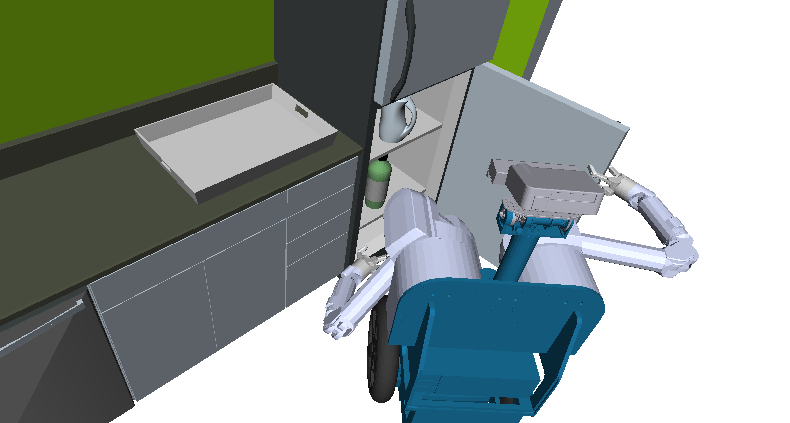
\includegraphics[width=2.5cm]{figs/fridge-intro.png}};
         \node[inner sep=0pt,anchor=north,align=center,font=\scriptsize] at (2.0,6) {$\sim10$k\\vertices};
      }
      \only<18->
      {
         \node[inner sep=0pt] at (5.0,7) {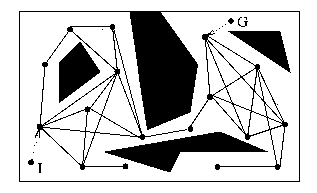
\includegraphics[width=2.5cm]{figs/prm.png}};
         \node[inner sep=0pt,anchor=north,align=center,font=\scriptsize] at (5.0,6)
            {Motivation: PRM};
         % cite
         %\node[anchor=east,font=\scriptsize] at (12,0.5)
         %   {$^\dag$ Kavraki, Svestka, Latombe, Overmars, 1996.};
      }
      
      % draw graph box
      \only<1-2>{
         \node[draw,align=center,minimum height=1.3cm,anchor=south east] at (5,3.5) {
            Graph\\$G = (V,E)$\\\includegraphics[width=1cm]{build/roadmap-2d-simple}
         };
      }
      \only<3-15>{
         \node[draw,align=center,minimum height=1.3cm,anchor=south east] at (5,3.5) {
            Graph\\$G = (V,E)$\\\includegraphics[width=3cm]{build/roadmap-2d-simple}
         };
      }
      % grow using a*!
      \only<7-14>{
         \fill[white,fill opacity=0.9] (1.8,3.6) rectangle (4.9,6.7);
         \begin{scope}
            \clip (1.8,3.6) rectangle (4.9,6.7);
            \only<7>{\clip[rotate around={15:(2.0,4.8)}] (2.0,4.8) ellipse (0.5cm and 0.25cm);}
            \only<8>{\clip[rotate around={15:(2.0,4.8)}] (2.0,4.8) ellipse (1.0cm and 0.50cm);}
            \only<9>{\clip[rotate around={15:(2.0,4.8)}] (2.0,4.8) ellipse (1.4cm and 0.70cm);}
            \only<10>{\clip[rotate around={15:(2.0,4.8)}] (2.0,4.8) ellipse (1.6cm and 0.80cm);}
            \only<11>{\clip[rotate around={15:(2.0,4.8)}] (2.0,4.8) ellipse (1.9cm and 0.85cm);}
            \only<12>{\clip[rotate around={15:(2.0,4.8)}] (2.0,4.8) ellipse (2.1cm and 1.05cm);}
            \only<13-14>{\clip[rotate around={15:(2.0,4.8)}] (2.0,4.8) ellipse (2.2cm and 1.10cm);}
            \node[align=center,minimum height=1.3cm,anchor=south east] at (5,3.5) {
               \includegraphics[width=3cm]{build/roadmap-2d-simple}};
            \only<14>{\draw[rotate around={15:(2.0,4.8)},line width=4pt]
               (2.0,4.8) ellipse (2.2cm and 1.10cm);}
         \end{scope}
      }
      \only<16->{
         \node[draw,align=center,minimum height=1.3cm,anchor=south east,font=\scriptsize] at (5,3.5) {
            Graph\\$G = (V,E)$\\\includegraphics[width=0.5cm]{build/roadmap-2d-simple}
         };
      }
      
      % draw edge eval box
      \only<1-2>{
         \node[draw,align=center,anchor=south west] at (7,3.5)
            {\\Edge Weight\\$x : E \rightarrow \mathbb{R}^+$\\};
      }
      \only<3-15>{
         \begin{scope}[font=\tiny]
            \node[draw,align=center,anchor=south west] at (7,3.5)
               {\\Edge Weight\\$x : E \rightarrow \mathbb{R}^+$\\};
         \end{scope}
      }
      \only<16->{
         \node[draw,align=center,anchor=south west,inner sep=1cm] at (7,3.5)
            {\\Edge Weight\\$x : E \rightarrow \mathbb{R}^+$\\};
      }
      
      \draw[->,line width=1pt] (4,3.25) -- (4,2.75);
      \draw[->,line width=1pt] (8,3.25) -- (8,2.75);
      \node[draw,align=center,minimum height=1.0cm,minimum width=5cm,anchor=north]
         at (6,2.5) {\\$GS(G,x)$};

      % clocks
      \only<2-13>{
         % graph
         \node[fill=white,circle,inner sep=-2pt] at (5,3.5) {\LARGE%
            \only<2-6>{\showclock{0}{0}}%
            \only< 7>{\showclock{0}{10}}%
            \only< 8>{\showclock{0}{20}}%
            \only< 9>{\showclock{0}{30}}%
            \only<10>{\showclock{0}{40}}%
            \only<11>{\showclock{0}{50}}%
            \only<12>{\showclock{1}{00}}%
            \only<13>{\showclock{1}{10}}%
         };
         % edge weight
         \node[fill=white,circle,inner sep=-2pt] at (7,3.5) {\LARGE%
            \only<2-6>{\showclock{0}{0}}%
            \only< 7>{\showclock{0}{5}}%
            \only< 8>{\showclock{0}{10}}%
            \only< 9>{\showclock{0}{15}}%
            \only<10>{\showclock{0}{20}}%
            \only<11>{\showclock{0}{25}}%
            \only<12>{\showclock{0}{30}}%
            \only<13>{\showclock{0}{35}}%
         };
         % graph search
         \node[fill=white,circle,inner sep=-2pt] at (6,2.5) {\LARGE%
            \only<2-6>{\showclock{0}{0}}%
            \only< 7>{\showclock{0}{5}}%
            \only< 8>{\showclock{0}{10}}%
            \only< 9>{\showclock{0}{20}}%
            \only<10>{\showclock{0}{40}}%
            \only<11>{\showclock{1}{20}}%
            \only<12>{\showclock{2}{40}}%
            \only<13>{\showclock{5}{20}}%
         };
      }
      \only<14>{
         % graph
         \node[fill=green,circle,inner sep=-2pt] at (5,3.5) {\LARGE\showclock{1}{10}};
         % edge weight
         \node[fill=white,circle,inner sep=-2pt] at (7,3.5) {\LARGE\showclock{0}{35}};
         % graph search
         \node[fill=white,circle,inner sep=-2pt] at (6,2.5) {\LARGE\showclock{5}{20}};
      }
      \only<15-18>{
         % graph
         \node[fill=white,circle,inner sep=-2pt] at (5,3.5) {\LARGE\showclock{0}{0}};
         % edge weight
         \node[fill=white,circle,inner sep=-2pt] at (7,3.5) {\LARGE\showclock{0}{0}};
         % graph search
         \node[fill=white,circle,inner sep=-2pt] at (6,2.5) {\LARGE\showclock{0}{0}};
      }
      \only<19->{
         % graph
         \node[fill=white,circle,inner sep=-2pt] at (5,3.5) {\LARGE\showclock{0}{0}};
         % edge weight
         \node[fill=green,circle,inner sep=-2pt] at (7,3.5) {\LARGE\showclock{0}{0}};
         % graph search
         \node[fill=white,circle,inner sep=-2pt] at (6,2.5) {\LARGE\showclock{0}{0}};
      }
      
      \node[draw,align=center,shape=document] at (1.5,2) {Query\;\;\;};
      \draw[->,line width=1pt] (2.5,2) -- (3.25,2);
      \draw[->,line width=1pt] (8.75,2) -- (9.50,2);
      \node[draw,align=center,shape=document] at (10.15,2) {$\pi^*$\;\;\;};

      \only<14>{
         \node at (6,0.75) {A* is {\bf optimally efficient} w.r.t
            the number of {\bf vertices considered}.};
      }
      \only<19>{
         \node at (6,0.75) {A* is {\bf not optimally efficient} w.r.t
            the number of {\bf edges evaluated}.
         };
      }
      \only<20>{
         \node[align=center] at (6,0.75) {
            The {\bf E$^4$} graph search problem:\\
            \emph{Explicit graphs with Expensive Edge Evaluations}
         };
      }
      
   \end{tikzpicture}
\end{frame}

\begin{frame}
   \frametitle{Explicit Graphs with Expensive Edge Evaluations}
   \begin{tikzpicture}
   
      \draw[step=1,black!10,very thin,opacity=\gridopacity] (0,0) grid (12,8);
      
      \node[inner sep=0] at (9.25,5) {%
         \includegraphics{build/talk-act1-2d,astara}%
      };
      
      % f(x) highlight
      \node[inner sep=0pt,fill=black!5,minimum height=2.8cm,minimum width=6.3cm,rounded corners]
         at (3.25,6.3) {};
      \only<3>{\fill[green!30] (0.1,5.85) rectangle (6.4,6.65);}
      
      % bfs
      \node[anchor=north west,inner sep=0pt] at (0.25,7.6) {Best-first search over paths:};
      \node[anchor=north,inner sep=0pt] at (3.25,7.0) {\begin{minipage}{6.5cm}\small{
         \algrenewcommand\algorithmicindent{0.2cm}%
         \begin{algorithmic}
         \Loop%
            \State ${\hat \pi}^* \leftarrow \argmin\limits_{\pi \in \Pi}
               \left[ \hat{f}_x(\pi) \right]$
            \State $e \leftarrow$ select from ${\hat \pi}^*$
            \State $x(e)$
         \EndLoop
         \end{algorithmic}
      }\end{minipage}};
      
      % fx(pi) execution path cost
      \node[anchor=north,inner sep=0pt] at (3.25,5.1) {\begin{minipage}{6cm}\small{
         \begin{equation*}
            \arraycolsep=1.4pt
            \hat{f}_x(\pi) = \sum_{e \in \pi} \left\{
            \begin{array}{cl}
               x(e) & \mbox{if edge } e \mbox{ evaluated}  \\
               \hat{x}(e) & \mbox{otherwise} \\
            \end{array}
            \right.
         \end{equation*}
      }\end{minipage}};
      
      % ensemble highlight
      \node[anchor=north,shape=document,draw,inner sep=0.25cm] at (6,2.25) {\begin{minipage}{8.5cm}\small{
         Effort model:
         
         $x(e)$ : edge evaluation function \emph{(expensive to compute)}
         
         ${\hat x}(e)$ : optimistic estimate of value of $x(e)$
      }\end{minipage}};
      
      \only<2>{
         \node[fill=white,opacity=0.9] at (9.25,3) {This is Lazy PRM! Animate!};
      }
   
   \end{tikzpicture}
\end{frame}

\begin{frame}
   \frametitle{Challenge 1: The Planning/Execution Tradeoff}
   \begin{tikzpicture}
   
      \draw[step=1,black!10,very thin,opacity=\gridopacity] (0,0) grid (12,8);
      
      \node[inner sep=0pt] at (3.5,5) {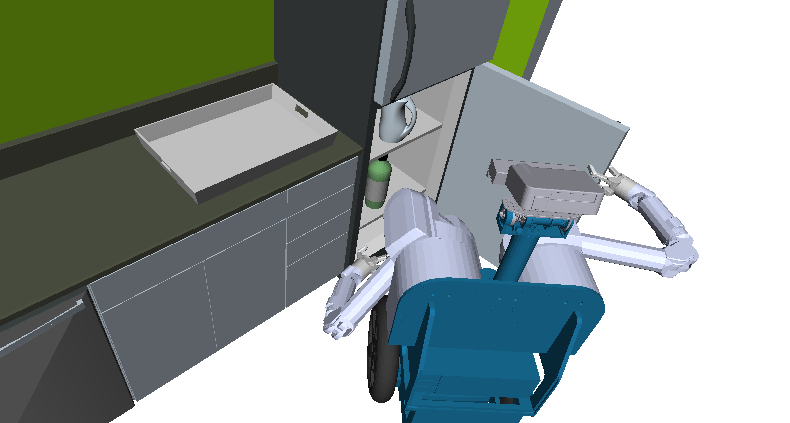
\includegraphics[width=4cm]{figs/fridge-intro.png}};
      \node[inner sep=0pt,anchor=north] at (3.5,3.5)
         {\begin{minipage}{4cm}\centering
            Our problem
            
            (plan then execute)
         \end{minipage}};
      
      \node[inner sep=0pt] at (8.5,4.5) {\includegraphics{build/ensemble-effort-plot-1}};
      
      
   \end{tikzpicture}
\end{frame}

\begin{frame}
   \frametitle{Explicit Graphs with Expensive Edge Evaluations}
   \begin{tikzpicture}
   
      \draw[step=1,black!10,very thin,opacity=\gridopacity] (0,0) grid (12,8);
      
      \node[inner sep=0] at (9.25,5) {%
         \includegraphics{build/talk-act1-2d,astara}%
      };
      
      % f(x) highlight
      \node[inner sep=0pt,fill=black!5,minimum height=2.8cm,minimum width=6.3cm,rounded corners]
         at (3.25,6.3) {};
      \only<4-6>{\fill[green!30] (2.65,5.9) rectangle (6.4,6.7);}
      
      % bfs
      \node[anchor=north west,inner sep=0pt] at (0.25,7.6) {Best-first search over paths:};
      \node[anchor=north,inner sep=0pt] at (3.25,7.0) {\begin{minipage}{6.5cm}\small{
         \algrenewcommand\algorithmicindent{0.2cm}%
         \begin{algorithmic}
         \Loop%
            \only<1-3>{
               \State ${\hat \pi}^* \leftarrow \argmin\limits_{\pi \in \Pi}
                  \left[ \hat{f}_x(\pi) \right]$
            }
            \only<4-6>{
               \State ${\hat \pi}^* \leftarrow \argmin\limits_{\pi \in \Pi}
                  \left[ (1-\lambda) \hat{f}_x(\pi) + \lambda \hat{f}_p(\pi) \right]$
            }
            \State $e \leftarrow$ select from ${\hat \pi}^*$
            \State $x(e)$
         \EndLoop
         \end{algorithmic}
      }\end{minipage}};
      
      % fx(pi) execution path cost
      \node[anchor=north,inner sep=0pt] at (3.25,5.1) {\begin{minipage}{6cm}\small{
         \begin{equation*}
            \arraycolsep=1.4pt
            \hat{f}_x(\pi) = \sum_{e \in \pi} \left\{
            \begin{array}{cl}
               x(e) & \mbox{if edge } e \mbox{ evaluated}  \\
               \hat{x}(e) & \mbox{otherwise} \\
            \end{array}
            \right.
         \end{equation*}
      }\end{minipage}};
      
      % fp(pi) execution path cost
      \only<3-6>{
      \fill[green!30] (0.1,2.5) rectangle (6.4,3.6);
      \node[anchor=north,inner sep=0pt] at (3.25,3.9) {\begin{minipage}{6cm}\small{
         \begin{equation*}
            \arraycolsep=1.4pt
            \hat{f}_p(\pi) = \sum_{e \in \pi} \left\{
            \begin{array}{cl}
               0 & \mbox{if edge } e \mbox{ evaluated}  \\
               \hat{p}(e) & \mbox{otherwise} \\
            \end{array}
            \right.
         \end{equation*}
      }\end{minipage}};
      }
      
      % p(e) highlight
      \only<2-6>{\fill[green!30] (1.5,0.3) rectangle (10.5,0.8);}
      % ensemble highlight
      \only<6>{\fill[green!30] (1.6,1.6) rectangle (5.3,2.1);}
      \node[anchor=north,shape=document,draw,inner sep=0.25cm] at (6,2.25) {\begin{minipage}{8.5cm}\small{
         \only<1-5>{Effort model:}
         \only<6>{\emph{Ensemble Effort} model:}
         
         $x(e)$ : edge evaluation function \emph{(expensive to compute)}
         
         ${\hat x}(e)$ : optimistic estimate of value of $x(e)$
         
         \only<2-6>{
            ${\hat p}(e)$ : optimistic estimate of evaluation cost of $x(e)$
         }
         
      }\end{minipage}};
      
      \only<5-6>{
         \node[fill=white,opacity=0.9] at (9.25,3) {Animate example!};
      }
   
   \end{tikzpicture}
\end{frame}

\begin{frame}
   \frametitle{The E$^8$ Algorithm}
   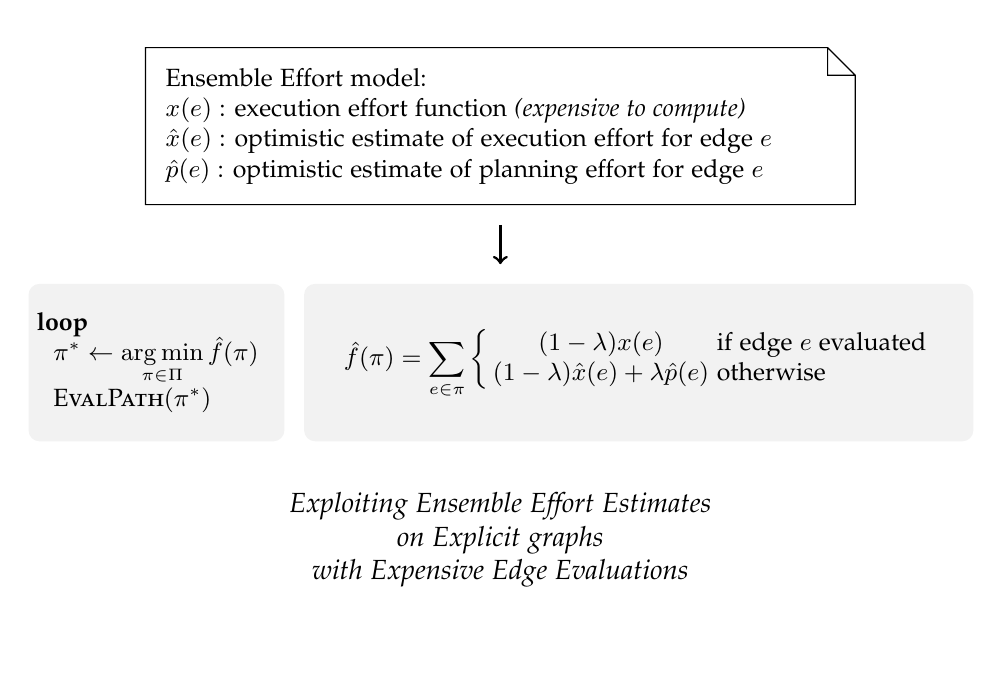
\begin{tikzpicture}
   
      \draw[step=1,black!10,very thin,opacity=\gridopacity] (0,0) grid (12,8);
      
      \node[anchor=north,shape=document,draw,inner sep=0.25cm] at (6,7.75) {\begin{minipage}{8.5cm}\small{
         Ensemble Effort model:
         
         $x(e)$ : execution effort function \emph{(expensive to compute)}
         
         ${\hat x}(e)$ : optimistic estimate of execution effort for edge $e$
         
         ${\hat p}(e)$ : optimistic estimate of planning effort for edge $e$
      }\end{minipage}};
      
      \draw[->,line width=1pt] (6,5.5) -- (6,5.0);
      
      % alg
      \node[anchor=west,inner xsep=0pt,fill=black!5,minimum height=2cm,rounded corners]
      at (0,3.75) {\begin{minipage}{3.25cm}\small{
         \algrenewcommand\algorithmicindent{0.0cm}%
         \algrenewcommand\algorithmicloop{\!\!\!\!\textbf{loop}}
         \begin{algorithmic}
         \Loop%
            \State $\pi^* \leftarrow \argmin\limits_{\pi \in \Pi} \hat{f}(\pi)$
            \State \textsc{EvalPath}$(\pi^*)$
         \EndLoop
         \end{algorithmic}
      }\end{minipage}};
      
      % f(pi) execution path cost
      \node[anchor=west,inner xsep=0pt,fill=black!5,minimum height=2cm,rounded corners]
      at (3.5,3.75) {\begin{minipage}{8.5cm}\small{%
         \vspace{-0.3cm}
         \begin{equation*}%
            \arraycolsep=1.4pt
            \hat{f}(\pi) = \sum_{e \in \pi} \left\{
            \begin{array}{cl}
               (1-\lambda) x(e) & \mbox{if edge } e \mbox{ evaluated} \\
               (1-\lambda) \hat{x}(e) + \lambda \hat{p}(e) & \mbox{otherwise} \\
            \end{array}
            \right.
         \end{equation*}
      }\end{minipage}};
      
      \node[inner sep=0pt] at (6,1.5) {\begin{minipage}{12cm}\centering
         \emph{Exploiting Ensemble Effort Estimates\\
         on Explicit graphs\\
         with Expensive Edge Evaluations}
      \end{minipage}};
   
   \end{tikzpicture}
\end{frame}

\begin{frame}
   \frametitle{Example Problem}
   \begin{tikzpicture}
   
      \draw[step=1,black!10,very thin,opacity=\gridopacity] (0,0) grid (12,8);
      
      \node[inner sep=0pt] at (6,4.75) {%
         \only<1>{\includegraphics[width=6cm]{build/e8-world-intro}}%
         \only<2>{\includegraphics[width=6cm]{build/e8-world-astar}}%
         \only<3>{\includegraphics[width=6cm]{build/e8-world-wastar}}%
         \only<4>{\includegraphics[width=6cm]{build/e8-world-e8}}%
      };
      
      \node[inner sep=0pt] at (6,0.75) {\begin{minipage}{6cm}\centering%
         \only<2>{
            Planning Effort: 692.3 \\%\worldstatsastarplan\\
            Execution Effort: 14.2 \\%\worldstatsastarexec\\
            Total Effort: 706.5
         }
         \only<3>{
            Planning Effort: 390.8 \\%\worldstatswastarplan\\
            Execution Effort: 18.5 \\%\worldstatswastarexec\\
            Total Effort: 409.3
         }
         \only<4>{
            Planning Effort: 358.8 \\%\worldstatseEplan\\
            Execution Effort: 20.5 \\%\worldstatseEexec\\
            Total Effort: 379.3
         }
      \end{minipage}};
      
   \end{tikzpicture}
\end{frame}

\begin{frame}
   \frametitle{Simplification with Proportional Heuristics}
   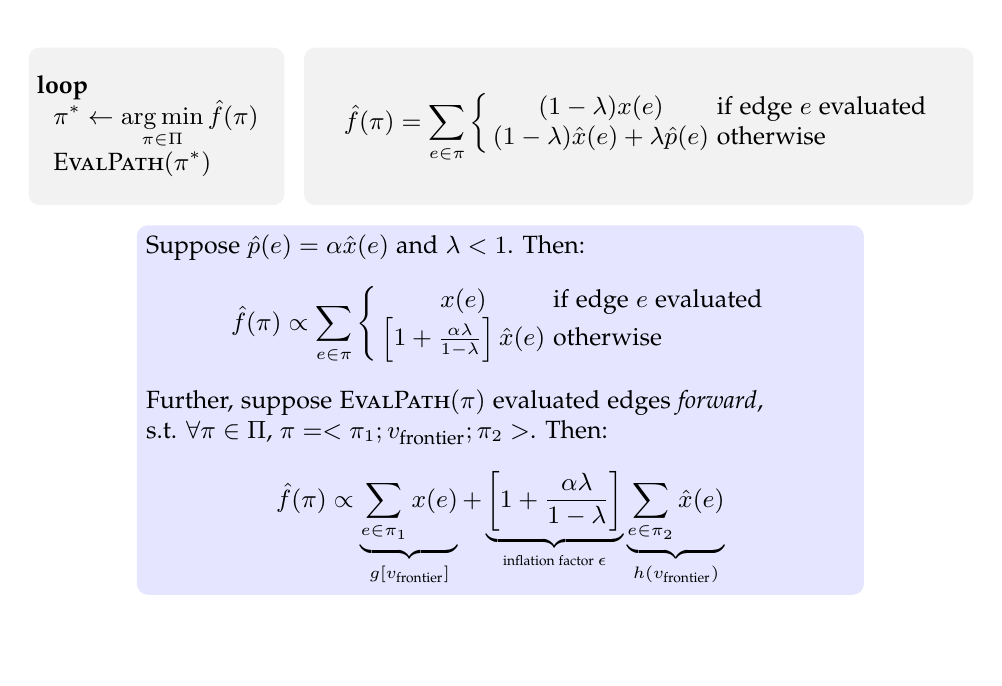
\begin{tikzpicture}
   
      \draw[step=1,black!10,very thin,opacity=\gridopacity] (0,0) grid (12,8);
      
      % alg
      \node[anchor=west,inner xsep=0pt,fill=black!5,minimum height=2cm,rounded corners]
      at (0,6.75) {\begin{minipage}{3.25cm}\small{
         \algrenewcommand\algorithmicindent{0.0cm}%
         \algrenewcommand\algorithmicloop{\!\!\!\!\textbf{loop}}
         \begin{algorithmic}
         \Loop%
            \State $\pi^* \leftarrow \argmin\limits_{\pi \in \Pi} \hat{f}(\pi)$
            \State \textsc{EvalPath}$(\pi^*)$
         \EndLoop
         \end{algorithmic}
      }\end{minipage}};
      
      % f(pi) execution path cost
      \node[anchor=west,inner xsep=0pt,fill=black!5,minimum height=2cm,rounded corners]
      at (3.5,6.75) {\begin{minipage}{8.5cm}\small{%
         \vspace{-0.3cm}
         \begin{equation*}%
            \arraycolsep=1.4pt
            \hat{f}(\pi) = \sum_{e \in \pi} \left\{
            \begin{array}{cl}
               (1-\lambda) x(e) & \mbox{if edge } e \mbox{ evaluated} \\
               (1-\lambda) \hat{x}(e) + \lambda \hat{p}(e) & \mbox{otherwise} \\
            \end{array}
            \right.
         \end{equation*}
      }\end{minipage}};
      
      % supposition box
      \node[anchor=north,fill=blue!10,rounded corners] at (6,5.5) {\begin{minipage}{9cm}\small{
         Suppose ${\hat p}(e) = \alpha {\hat x}(e)$ and $\lambda < 1$.
         Then:
         \begin{equation*}
            \arraycolsep=1.4pt
            \hat{f}(\pi) \propto \sum_{e \in \pi} \left\{
            \begin{array}{cl}
               x(e) & \mbox{if edge } e \mbox{ evaluated} \\
               \left[ 1 + \frac{\alpha \lambda}{1-\lambda} \right] \hat{x}(e) & \mbox{otherwise} \\
            \end{array}
            \right.
         \end{equation*}
         
         Further, suppose \textsc{EvalPath}$(\pi)$ evaluated edges \emph{forward},\\
         s.t. $\forall \pi \in \Pi$,
         $\pi = < \pi_1; v_{\ms{frontier}}; \pi_2 >$.
         Then:
         \begin{equation*}
            \hat{f}(\pi) \propto
            \underbrace{
               \sum_{e \in \pi_1} x(e)
            }_{g[v_{\mbox{\tiny frontier}}]}
            +
            \underbrace{
               \left[ 1 + \frac{\alpha \lambda}{1-\lambda} \right]
            }_{\mbox{\tiny inflation factor } \epsilon}
            \underbrace{
               \sum_{e \in \pi_2} \hat{x}(e)
            }_{h(v_{\mbox{\tiny frontier}})}
         \end{equation*}
         
      }\end{minipage}};
   
   \end{tikzpicture}
\end{frame}

\begin{frame}
   \frametitle{Algorithm Comparison}
   \begin{tikzpicture}
      \draw[step=1,black!10,very thin,opacity=\gridopacity] (0,0) grid (12,8);
      
      \draw[line width=1pt] (1,7) -- (11,7);
      
      \node[align=center] at (2,6.25) {Heuristic\\Estimates};
      \node[align=center] at (5.5,6.25) {Implicit Graphs\\(search over vertices)};
      \node[align=center] at (9.5,6.25) {E$^4$ Graphs\\(search over paths)};
      
      \draw[line width=0.1pt] (1,5.6) -- (11,5.6);
      
      \node[anchor=west] at (1.5,5) {none};
      \node[anchor=west] at (1.5,4) {${\hat x}$};
      
      \draw[line width=0.1pt] (1,1.4) -- (11,1.4);
      
      \only<2->{
         \node[fill=black!5,rounded corners,minimum height=0.8cm,minimum width=3cm]
            at (5.5,5) {Dijkstra's};
         \node[fill=black!5,rounded corners,minimum height=0.8cm,minimum width=3cm]
            at (5.5,4) {A*};
      }
      \only<3->{
         \node[fill=black!5,rounded corners,minimum height=0.8cm,minimum width=3cm]
            at (9.5,4) {Lazy PRM};
      }
      
      \only<4->{
         \node[anchor=west] at (1.5,2) {${\hat x}, \; {\hat p}$};
         \node[fill=black!5,rounded corners,minimum height=1.8cm,minimum width=3cm]
            at (9.5,2.5) {E$^8$};
      }
      
      \only<5->{
         \node[anchor=west] at (1.5,3) {${\hat x}, \; {\hat p} \propto {\hat x}$};
         \node[fill=black!5,rounded corners,minimum height=0.8cm,minimum width=3cm]
            at (5.5,3) {Weighted A*};
      }
      
      \only<6->{
         \node[fill=black!5,rounded corners,minimum height=0.8cm,minimum width=3cm]
            at (5.5,2) {BUGSY$^\dag$};
         \node at (6,0.5) {\begin{minipage}{9cm}\scriptsize{
            $^\dag$ W. Ruml and M. B. Do. Best-first Utility-Guided Search.\\
            International Joint Conference on Artificial Intelligence, 2007.
         }\end{minipage}};
      }
      
   \end{tikzpicture}
\end{frame}

\begin{frame}
   \frametitle{Suboptimality Guarantees}
   \begin{tikzpicture}
   
      \draw[step=1,black!10,very thin,opacity=\gridopacity] (0,0) grid (12,8);
      
      % alg
      \node[anchor=west,inner xsep=0pt,fill=black!5,minimum height=2cm,rounded corners]
      at (0,6.75) {\begin{minipage}{3.25cm}\small{
         \algrenewcommand\algorithmicindent{0.0cm}%
         \algrenewcommand\algorithmicloop{\!\!\!\!\textbf{loop}}
         \begin{algorithmic}
         \Loop%
            \State $\pi^* \leftarrow \argmin\limits_{\pi \in \Pi} \hat{f}(\pi)$
            \State \textsc{EvalPath}$(\pi^*)$
         \EndLoop
         \end{algorithmic}
      }\end{minipage}};
      
      % f(pi) execution path cost
      \node[anchor=west,inner xsep=0pt,fill=black!5,minimum height=2cm,rounded corners]
      at (3.5,6.75) {\begin{minipage}{8.5cm}\small{%
         \vspace{-0.3cm}
         \begin{equation*}%
            \arraycolsep=1.4pt
            \hat{f}(\pi) = \sum_{e \in \pi} \left\{
            \begin{array}{cl}
               (1-\lambda) x(e) & \mbox{if edge } e \mbox{ evaluated} \\
               (1-\lambda) \hat{x}(e) + \lambda \hat{p}(e) & \mbox{otherwise} \\
            \end{array}
            \right.
         \end{equation*}
      }\end{minipage}};
      
      % supposition box
      \only<2->{
         \node[anchor=north,fill=blue!10,rounded corners] at (6,5.5) {\begin{minipage}{9cm}\small{
            {\bf Theorem:}
            If ${\hat p}(e) \leq A {\hat x}(e)$,
            then the solution path returned by E$^8$
            is at most $1 + \frac{A \lambda}{1-\lambda}$ times
            the cost of the optimal path.
         }\end{minipage}};
      }
      
      % research question
      \only<3->{
         \node[anchor=north,fill=blue!20,rounded corners] at (6,4) {\begin{minipage}{9cm}
            {\bf Research Question Q1:}\\
            Can we make any non-trivial guarantees for E$^8$ w.r.t.
            \begin{itemize}
            \item solution quality (execution effort),
            \item accumulated planning effort, or
            \item $\lambda$-mediated tradoff between the two?
            \end{itemize}
         \end{minipage}};
      }
   
   \end{tikzpicture}
\end{frame}

\begin{frame}
   \frametitle{Na\"{\i}ve Implementation}
   \begin{tikzpicture}
      \draw[step=1,black!10,very thin,opacity=\gridopacity] (0,0) grid (12,8);
   
      \only<1-4>{
         % alg
         \node[anchor=west,inner xsep=0pt,fill=black!5,minimum height=1.8cm,rounded corners]
         at (0,6.75) {\begin{minipage}{3.25cm}\small{
            \algrenewcommand\algorithmicindent{0.0cm}%
            \algrenewcommand\algorithmicloop{\!\!\!\!\textbf{loop}}
            \begin{algorithmic}
            \Loop%
               \State $\pi^* \leftarrow \argmin\limits_{\pi \in \Pi} \hat{f}(\pi)$
               \State \textsc{EvalPath}$(\pi^*)$
            \EndLoop
            \end{algorithmic}
         }\end{minipage}};
         
         % f(pi) execution path cost
         \node[anchor=west,inner xsep=0pt,fill=black!5,minimum height=1.8cm,rounded corners]
         at (3.5,6.75) {\begin{minipage}{8.5cm}\small{%
            \vspace{-0.3cm}
            \begin{equation*}%
               \arraycolsep=1.4pt
               \hat{f}(\pi) = \sum_{e \in \pi} \left\{
               \begin{array}{cl}
                  (1-\lambda) x(e) & \mbox{if edge } e \mbox{ evaluated} \\
                  (1-\lambda) \hat{x}(e) + \lambda \hat{p}(e) & \mbox{otherwise} \\
               \end{array}
               \right.
            \end{equation*}
         }\end{minipage}};
      }
      
      % research question
      \only<5>{
         \node[fill=blue!20,rounded corners] at (6,6.75) {\begin{minipage}{9cm}
            {\bf Research Question Q2:}\\
            How can incremental graph search ideas (e.g. LPA*)\\be used to
            efficiently implement the E$^8$ algorithm?
         \end{minipage}};
      }
      
      % procedure background
      \only<2->{
         \node[fill=blue!10,rounded corners,minimum height=5.1cm,minimum width=11.4cm]
         at (6,3.1) {};
      }
      
      % procedure background highlights
      \only<3->{\fill[red!30] (0.3,1.075) rectangle (11.7,1.575);}
      \only<4->{\fill[green!30] (0.3,2.80) rectangle (11.7,3.30);}
      
      % procedure itself
      \only<2->{
         \node[inner sep=0] at (6,3.1) {\begin{minipage}{11cm}\small{
         \begin{algorithmic}[1]
            \Procedure {E$^8$}{$G,
               V_{\mbox{\scriptsize start}}, V_{\mbox{\scriptsize goal}},
               \mathcal{M}, \lambda$}
            \State $x_{\mbox{\scriptsize eval}}[\cdot] \leftarrow$ empty map
               ($E \rightarrow \mathbb{R}_0^+$)
            \ForAll {$e \in G$}
               \State $e.{\mbox{cost}} \leftarrow
                  (1 - \lambda) \, \hat{x}(e) + \lambda \, \hat{p}(e)$
                  \Comment Ensemble effort model
            \EndFor
            \Loop
               \State $\pi^* = \mbox{\sc BiDijkstras}(G,
                  V_{\mbox{\scriptsize start}}, V_{\mbox{\scriptsize goal}})$
               \State $e \leftarrow \mbox{select from } \pi
                  \;|\; e \notin x_{\mbox{\scriptsize eval}}$
               \If {$e = \mbox{\bf nil}$}
                  \State \Return $\pi^*$
               \EndIf
               \State $x_{\mbox{\scriptsize eval}}[e] \leftarrow x(e)$
                  \Comment Evaluate edge (expensive!)
               \State $e.{\mbox{cost}} \leftarrow
                  (1 - \lambda) \, x_{\mbox{\scriptsize eval}}[e]$
                  \Comment Update ensemble estimate
            \EndLoop
            \EndProcedure
         \end{algorithmic}
         }\end{minipage}};
      }
      
   \end{tikzpicture}
\end{frame}

\begin{frame}
   \frametitle{Multiple Queries}
   \begin{tikzpicture}
      \draw[step=1,black!10,very thin,opacity=\gridopacity] (0,0) grid (12,8);
      
      \node[inner sep=0pt] at (6,7.4) {\begin{minipage}{12cm}\centering
         Implicit algorithms manifest planning effort in
         {\bf computed g-values}.
         Explicit algorithms manifest planning effort in
         {\bf evaluated edges}.
      \end{minipage}};
      
      \begin{scope}[shift={(0,0.8)}]
         \clip (0,4.5) rectangle (12,6);
         \node[fill=blue!10,rounded corners,minimum height=5.8cm,minimum width=8.4cm] at (6,3) {};
         \node[inner sep=0,anchor=north] at (6,5.8) {\begin{minipage}{8cm}\small{
         \begin{algorithmic}[1]
            \Procedure {E$^8$}{$G,
               V_{\mbox{\scriptsize start}}, V_{\mbox{\scriptsize goal}},
               \mathcal{M}, \lambda$}
            \State $x_{\mbox{\scriptsize eval}}[\cdot] \leftarrow$ empty map
               ($E \rightarrow \mathbb{R}_0^+$)
            \State $\dots$
            \EndProcedure
         \end{algorithmic}
         }\end{minipage}};
      \end{scope}
      
      \node[inner sep=0] at (3,2.6) {
         \includegraphics{build/talk-act1-2d,astars}
      };
      \node[inner sep=0] at (9,2.6) {
         \includegraphics{build/talk-act1-2d,astars}
      };
   
   \end{tikzpicture}
\end{frame}

\begin{frame}
   \frametitle{Multiple Queries: Relationship to Experience Graphs}
   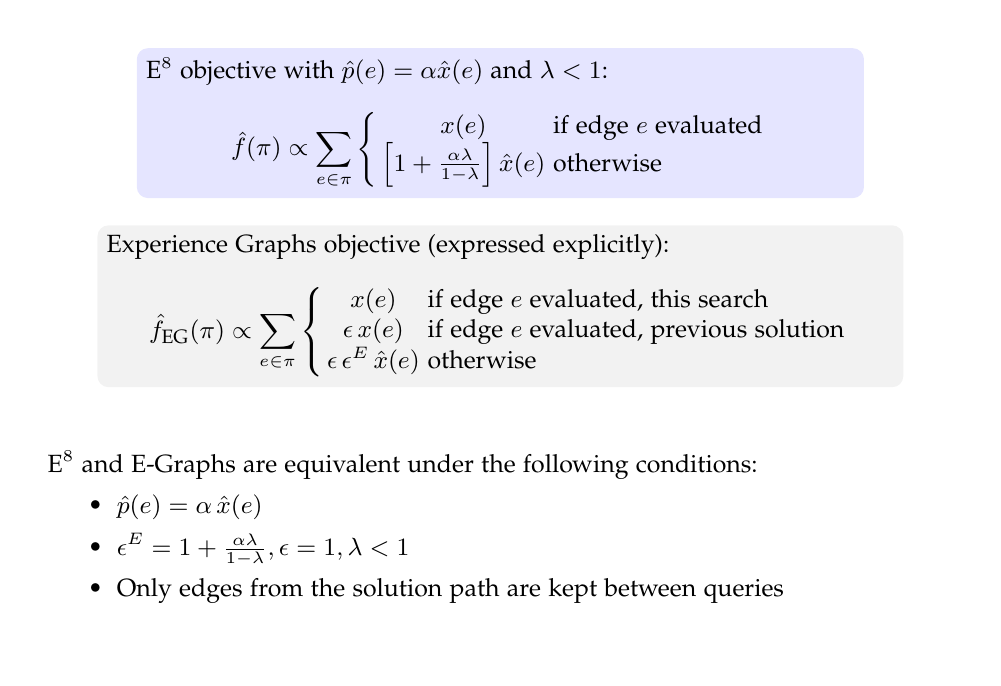
\begin{tikzpicture}
      \draw[step=1,black!10,very thin,opacity=\gridopacity] (0,0) grid (12,8);
      
      \node[anchor=north,fill=blue!10,rounded corners] at (6,7.75) {\begin{minipage}{9cm}\small{
         E$^8$ objective with ${\hat p}(e) = \alpha {\hat x}(e)$ and $\lambda < 1$:
         \begin{equation*}
            \arraycolsep=1.4pt
            \hat{f}(\pi) \propto \sum_{e \in \pi} \left\{
            \begin{array}{cl}
               x(e) & \mbox{if edge } e \mbox{ evaluated} \\
               \left[ 1 + \frac{\alpha \lambda}{1-\lambda} \right] \hat{x}(e) & \mbox{otherwise} \\
            \end{array}
            \right.
         \end{equation*}
      }\end{minipage}};
      
      \node[anchor=north,fill=black!5,rounded corners] at (6,5.5) {\begin{minipage}{10cm}\small{
         Experience Graphs objective (expressed explicitly):
         \begin{equation*}
            \arraycolsep=1.4pt
            \hat{f}_{\ms{EG}}(\pi) \propto \sum_{e \in \pi} \left\{
            \begin{array}{cl}
               x(e) & \mbox{if edge } e \mbox{ evaluated, this search} \\
               \epsilon \, x(e) & \mbox{if edge } e \mbox{ evaluated, previous solution} \\
               \epsilon \, \epsilon^E \, \hat{x}(e) & \mbox{otherwise} \\
            \end{array}
            \right.
         \end{equation*}
      }\end{minipage}};
      
      \node[anchor=north] at (6,2.75) {\begin{minipage}{11.5cm}\small{
         E$^8$ and E-Graphs are equivalent under the following
         conditions:
         \begin{itemize}
         \item ${\hat p}(e) = \alpha \, {\hat x}(e)$
         \item $\epsilon^E = 1 + \frac{\alpha \lambda}{1-\lambda},
            \epsilon = 1, \lambda < 1$
         \item Only edges from the solution path are kept between queries
         \end{itemize}
      }\end{minipage}};
      
   \end{tikzpicture}
\end{frame}

\begin{frame}
   \frametitle{Multiple Queries: Relationship to Experience Graphs}
   \begin{tikzpicture}
      \draw[step=1,black!10,very thin,opacity=\gridopacity] (0,0) grid (12,8);
      
      \draw[line width=1pt] (0.5,7.5) -- (11.5,7.5);
      
      \node[align=center] at (3,6.95) {Experience Graphs};
      \node[align=center] at (9,7) {E$^8$ Search};
      
      \draw[line width=0.1pt] (0.5,6.5) -- (11.5,6.5);
      
      \only<2->{
         \node[fill=black!5,rounded corners] at (3,5.75) {\begin{minipage}{4.5cm}\centering\small{
            Only keeping solutions may introduce helpful bias
         }\end{minipage}};
         
         \node[fill=blue!10,rounded corners] at (9,5.75) {\begin{minipage}{4.5cm}\centering\small{
            Keeping all evaluated edges may improve performance
         }\end{minipage}};
      }
      
      \only<3->{
         \node[fill=black!5,rounded corners] at (3,4.5) {\begin{minipage}{4.5cm}\centering\small{
            More efficient for larger graphs (e.g. shortcuts)
         }\end{minipage}};
      }
      
      \only<4->{
         \node[fill=blue!10,rounded corners] at (9,4.5) {\begin{minipage}{4.5cm}\centering\small{
            $\lambda$ and ${\hat{p}}(e)$ may be easier to set than $\epsilon$ and $\epsilon^E$
         }\end{minipage}};
      }
      
      \only<5->{
         \node[fill=blue!10,rounded corners] at (9,3.1) {\begin{minipage}{4.5cm}\centering\small{
            Supports non-proportional planning/execution effort heuristics
         }\end{minipage}};
      }
      
      \only<6->{
         \node[fill=blue!20,rounded corners] at (6,1) {\begin{minipage}{9cm}
            {\bf Research Question Q3:}\\
            How does the explicit graph approach of E$^8$ compare to
            weighted and anytime implicit algorithms?
         \end{minipage}};
      }
      
   \end{tikzpicture}
\end{frame}

\begin{frame}
   \frametitle{E$^8$ Search Summary}
   \begin{tikzpicture}

      \draw[step=1,black!10,very thin,opacity=\gridopacity] (0,0) grid (12,8);

      \node[anchor=south,shape=document,draw,inner sep=0.25cm]
      at (4,4.5) {\begin{minipage}{5cm}\small{
         Ensemble Effort model $\mathcal{M}$: \\
         $x(e)$ : edge evaluation function \\
         ${\hat x}(e)$ : execution effort estimate \\
         ${\hat p}(e)$ : planning effort estimate
      }\end{minipage}};
      
      \node[anchor=south,shape=document,draw,align=center]
      at (9,4.5) {
         Graph G:\\
         \includegraphics[width=2.5cm]{build/roadmap-2d-simple}
         %\includegraphics[width=2.5cm]{build/talk-act1-2d,graph}
         
      };
      
      \draw[->,line width=1pt] (6.3,4.4) -- (6.3,3.9);
      \draw[->,line width=1pt] (7.8,4.4) -- (7.8,3.9);
      
      \node[fill=blue!10,minimum height=1.5cm,minimum width=2.5cm,
         align=center,rounded corners,inner ysep=0.7cm]
      at (7,2.5) {
         E$^8$ Search\\
         \small{$\min
         \left[ (1 - \lambda) \hat{f}_x + \lambda \hat{f}_p \right]$}
      };
      
      \node[shape=document,draw,align=center,inner xsep=10pt]
      at (2.4,3) {
         Query $V_{s1}$, $V_{g1}$, $\lambda_1$
      };
      \draw[->,line width=1pt] (4.5,3) -- (5.0,3);
      
      \draw[->,line width=1pt] (9,3) -- (9.5,3);
      \node[shape=document,draw,align=center,inner xsep=5pt]
      at (10.1,3) {$\pi^*_1$\;\;};
      
      \node[shape=document,draw,align=center,inner xsep=10pt]
      at (2.4,2) {
         Query $V_{s2}$, $V_{g2}$, $\lambda_2$
      };
      \draw[->,line width=1pt] (4.5,2) -- (5.0,2);
      
      \draw[->,line width=1pt] (9,2) -- (9.5,2);
      \node[shape=document,draw,align=center,inner xsep=5pt]
      at (10.1,2) {$\pi^*_2$\;\;};

   \end{tikzpicture}
\end{frame}

\begin{frame}
   \frametitle{Continuous Spaces: Ensemble Effort Models}
   \begin{tikzpicture}
   
      \draw[step=1,black!10,very thin,opacity=\gridopacity] (0,0) grid (12,8);
      
      \node at (3,6.75) {e.g. $\mathcal{M} = \mathcal{M}_{\ms{dist}}
         + \mathcal{M}_{\ms{valid}}(\mathcal{C}_{\ms{free}})$};
      
      \node[inner sep=0] at (8,6.75) {%
         \includegraphics[width=2cm]{build/talk-act1-2d,graph}
      };
      \node[draw,line width=1.0pt,fill=blue!20,minimum width=0.75cm,minimum height=0.10cm]
         (Cfreebox) at (9.75, 6) {};
      \node[right=0cm of Cfreebox] {: $\mathcal{C}_{\ms{free}}$}; 
      
      \node[draw,shape=document,anchor=north] at (3,5.5) {
         \begin{minipage}[t]{5.5cm}%
            \vspace{0.1cm}
            Distance Model $\mathcal{M}_{\ms{dist}}$
            \begin{algorithmic}[1]
            \Function {$x_{\ms{\textup{dist}}}$}{$e$}
               \State \Return $|| q_e(1) - q_e(0) ||$
            \EndFunction
            \Function {$\hat{x}_{\ms{\textup{dist}}}$}{$e$}
               \State \Return $|| q_e(1) - q_e(0) ||$
            \EndFunction
            \Function {$\hat{p}_{\ms{\textup{dist}}}$}{$e$}
               \State \Return $0$
            \EndFunction
            \end{algorithmic}
         \end{minipage}%
      };
      
      \node[draw,shape=document,anchor=north] at (9,5.5) {
         \begin{minipage}[t]{5.5cm}%
            \vspace{0.1cm}
            Set Validity Model $\mathcal{M}_{\ms{valid}}(\mathcal{C}_{\ms{free}})$
            \begin{algorithmic}[1]
            \Function {$x_{\ms{\textup{valid}}}$}{$e, \mathcal{C}_{\ms{free}}$}
               \If {${\bf 1}_{\ms{free}}[q_e(t)]$}
                  \State \Return $0$
               \Else
                  \State \Return $\infty$
               \EndIf
            \EndFunction
            \Function {$\hat{x}_{\ms{\textup{valid}}}$}{$e, \mathcal{C}_{\ms{free}}$}
               \State \Return $0$
            \EndFunction
            \Function {$\hat{p}_{\ms{\textup{valid}}}$}{$e, \mathcal{C}_{\ms{free}}$}
               \State \Return $\hat{p}_{\ms{\textup{free}}}[q_e(t)]$
            \EndFunction
            \end{algorithmic}
         \end{minipage}%
      };
      
   \end{tikzpicture}
\end{frame}

\begin{frame}
   \frametitle{Continuous Spaces: E$^8$-PRM}
   \begin{tikzpicture}
      \draw[step=1,black!10,very thin,opacity=\gridopacity] (0,0) grid (12,8);
      
      \node[inner sep=0pt] at (6,7.4) {\begin{minipage}{11.5cm}\centering
         E$^8$ is agnostic to the type of roadmap used.
      \end{minipage}};
      
      \node[inner sep=0] at (4,5.5) {%
         \includegraphics[height=2.5cm]{build/roadmap-2d-densified}
      };
      
      \node[inner sep=0] at (8,5.5) {%
         \includegraphics[height=2.5cm]{figs/halton.png}
      };
      
      % procedure itself
      \node[fill=blue!10,rounded corners] at (6,2) {\begin{minipage}{11cm}\small{
         \begin{algorithmic}[1]
         \State $G \leftarrow \mbox{empty graph}$
         \State $\mathcal{M} \leftarrow
            \mathcal{M}_{\ms{dist}}
            + \mathcal{M}_{\ms{valid}}(\mathcal{C}_{\ms{free}})$
         \Procedure {E$^8$-PRM}{$G,
            V_{\mbox{\scriptsize start}}, V_{\mbox{\scriptsize goal}},
            N, \mathcal{M}, \lambda$}
         \State \textsc{AddRoots}($G, V_{\mbox{\scriptsize start}}, V_{\mbox{\scriptsize goal}}$)
         \Loop
            \State \textsc{PRMAddSamples}($G, \mathcal{C}, N$)
            \State $\pi^* \leftarrow \mbox{E}^8(G,
               V_{\mbox{\scriptsize start}}, V_{\mbox{\scriptsize goal}},
               \mathcal{M}, \lambda)$
            \If {$\mathcal{M}.\hat{x}(\pi^*) < \infty$}
               \State \Return $\pi^*$
            \EndIf
         \EndLoop
         \EndProcedure
         \end{algorithmic}
      }\end{minipage}};
      
   \end{tikzpicture}
\end{frame}

\begin{frame}
   \frametitle{Behavior of the E$^8$-PRM: Solution Paths}
   \begin{tikzpicture}
      \draw[step=1,black!10,very thin,opacity=\gridopacity] (0,0) grid (12,8);
   
      \node[draw,color=black!25,inner sep=1pt] (lambda0) at (3,6) {
         \includegraphics[width=5cm]{figs/bean-allpaths-lambda0.png}
      };
      \node[font=\small,below left=0cm of lambda0.north east] {$\lambda = 0$};
      
      \node[draw,color=black!25,inner sep=1pt] (lambda1) at (3,2) {
         \includegraphics[width=5cm]{figs/bean-allpaths-lambda1.png}
      };
      \node[font=\small,below left=0cm of lambda1.north east] {$\lambda = 1$};
      
      \begin{scope}[shift={(7.5,2.5)},font=\small]
      \begin{axis}[
         xlabel=Collision Checks,
         ylabel=Path Length,
         ylabel near ticks,
         xlabel near ticks,
         scaled x ticks=base 10:-3,
         scaled y ticks=base 10:-2,
         every x tick scale label/.style={
            at={(1,-0.2075)}
         },
         %ticks=none,
         axis lines=left,
         xmin=0,xmax=8000,
         ymin=700,ymax=950,
         width=5.5cm, height=5.5cm]
      
      \addplot[mark=*] plot coordinates { (7219.5, 733.0) };
      \addplot[mark=*] plot coordinates { (4692.6, 836.5) };
      \coordinate (l0) at (axis cs:7219.5, 733.0);
      \coordinate (l1) at (axis cs:4692.6, 836.5);
      
      \node (labl0) at ($ (l0) + (-250,15) $) {$\lambda=0$};
      \node (labl1) at ($ (l1) + (-250,15) $) {$\lambda=1$};
      \draw[->] (labl0) -- ($ (l0)!0.25cm!(labl0) $);
      \draw[->] (labl1) -- ($ (l1)!0.25cm!(labl1) $);

      \end{axis}
      \end{scope}
   
   \end{tikzpicture}
\end{frame}

\begin{frame}
   \frametitle{Behavior of the E$^8$-PRM: Maze RRT Comparison}
   \begin{tikzpicture}
      \draw[step=1,black!10,very thin,opacity=\gridopacity] (0,0) grid (12,8);
      
      % e8 prm on left side top
      \fill[blue!50] (0.1,2.8) rectangle (2.7,7.9);
      \node[inner sep=0pt] (lambda0) at (1.4,6.6) {
         \includegraphics[width=2.5cm]{figs/compare-2d-rrtc1-checkmask-l00-s1.png}
      };
      \node[font=\scriptsize,below left=0cm of lambda0.north east] {$\lambda = 0$};
      \node[inner sep=0pt] (lambda1) at (1.4,4.1) {
         \includegraphics[width=2.5cm]{figs/compare-2d-rrtc1-checkmask-l10-s1.png}
      };
      \node[font=\scriptsize,below left=0cm of lambda1.north east] {$\lambda = 1$};
      
      % rrts along bottom
      \fill[red!50] (1.15,0.1) rectangle (6.4,2.7);
      \node[inner sep=0pt] (conconr1) at (2.5,1.4) {
         \includegraphics[width=2.5cm]{figs/compare-2d-rrtc1-rrtconcon-r1-s1.png}
      };
      \node[font=\scriptsize,below left=0cm of conconr1.north east] {$R = 1$};
      \node[inner sep=0pt] (conconr6) at (5.05,1.4) {
         \includegraphics[width=2.5cm]{figs/compare-2d-rrtc1-rrtconcon-r6-s1.png}
      };
      \node[font=\scriptsize,below left=0cm of conconr6.north east] {$R = 6$};
      \fill[green!50] (6.65,0.1) rectangle (11.9,2.7);
      \node[inner sep=0pt] (extconr1) at (8.0,1.4) {
         \includegraphics[width=2.5cm]{figs/compare-2d-rrtc1-rrtextcon-r1-s1.png}
      };
      \node[font=\scriptsize,below left=0cm of extconr1.north east] {$R = 1$};
      \node[inner sep=0pt] (extconr6) at (10.55,1.4) {
         \includegraphics[width=2.5cm]{figs/compare-2d-rrtc1-rrtextcon-r6-s1.png}
      };
      \node[font=\scriptsize,below left=0cm of extconr6.north east] {$R = 6$};

      % plot
      \node[inner sep=0pt] at (7.5,5.25) {
         \includegraphics[width=9cm]{build/maze-plot-ensemble}
      };
      
   \end{tikzpicture}
\end{frame}

\begin{frame}
   \frametitle{HERB Example Problem}
   \begin{tikzpicture}
      \draw[step=1,black!10,very thin,opacity=\gridopacity] (0,0) grid (12,8);
   
      \node[inner sep=0pt]
         at ( 1.50,6.5) {\includegraphics[width=2cm]{figs/testherb-a.png}};
      \node[inner sep=0pt]
         at ( 3.75,6.5) {\includegraphics[width=2cm]{figs/testherb-b.png}};
      \node[inner sep=0pt]
         at ( 6.00,6.5) {\includegraphics[width=2cm]{figs/testherb-c.png}};
      \node[inner sep=0pt]
         at ( 8.25,6.5) {\includegraphics[width=2cm]{figs/testherb-d.png}};
      \node[inner sep=0pt]
         at (10.50,6.5) {\includegraphics[width=2cm]{figs/testherb-e.png}};

      \node[inner sep=0pt]
         at ( 2,3) {\includegraphics[width=3.9cm]{build/herb-mugbin-plot-1-eprm}};
      \node[inner sep=0pt]
         at ( 6,3) {\includegraphics[width=3.9cm]{build/herb-mugbin-plot-2-eprm}};
      \node[inner sep=0pt]
         at ( 10,3) {\includegraphics[width=3.9cm]{build/herb-mugbin-plot-3-eprm}};
   
   \end{tikzpicture}
\end{frame}

\begin{frame}
   \frametitle{Experiments in 2D and 7D}
   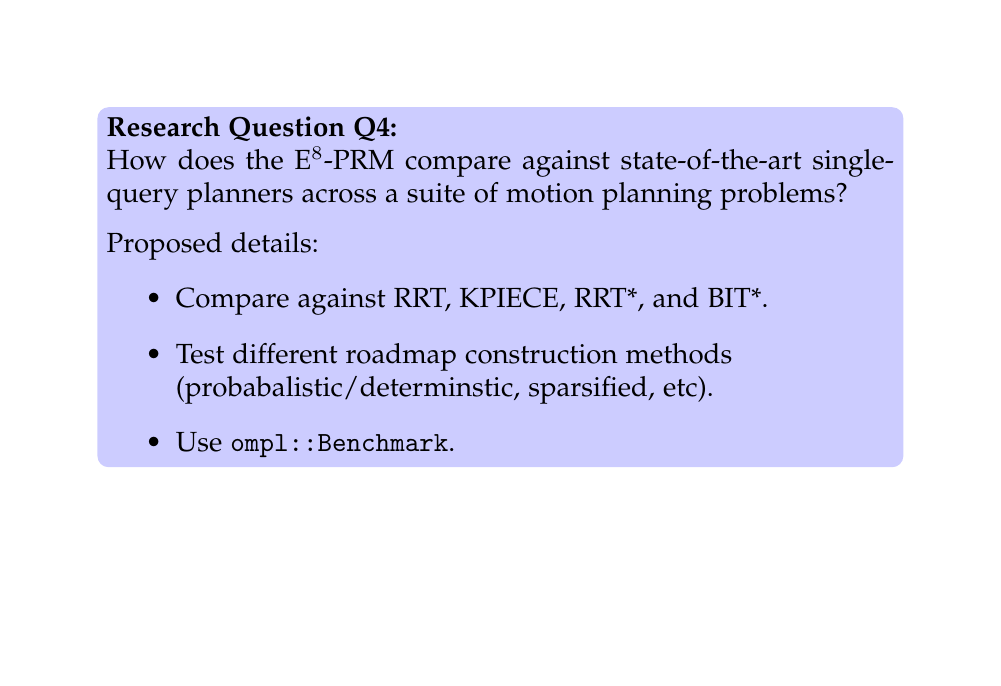
\begin{tikzpicture}
      \draw[step=1,black!10,very thin,opacity=\gridopacity] (0,0) grid (12,8);
   
      \node[anchor=north,fill=blue!20,rounded corners] at (6,7) {\begin{minipage}{10cm}
         {\bf Research Question Q4:}\\
         How does the E$^8$-PRM compare against state-of-the-art
         single-query planners across a suite of motion planning problems?
         
         \medskip
         Proposed details:
         \begin{itemize}
         \item Compare against RRT, KPIECE, RRT*, and BIT*.
         \item Test different roadmap construction methods \\
            (probabalistic/determinstic, sparsified, etc).
         \item Use {\tt ompl::Benchmark}.
         \end{itemize}
      \end{minipage}};
   
   \end{tikzpicture}
\end{frame}

\begin{frame}
   \frametitle{Roadmaps: Accounting for Spatial Coherence in $\mathcal{C}_{\ms{free}}$}
   \begin{tikzpicture}
   
      \draw[step=1,black!10,very thin,opacity=\gridopacity] (0,0) grid (12,8);
      
      \node[inner sep=0] at (9.4,5) {
         \includegraphics{build/talk-act1-2d,graphfirstevaled}
      };
      
      \node[anchor=north,fill=black!5,rounded corners]
      at (3.4,7.5) {\begin{minipage}{6.3cm}\small{
         Best First Search over paths:
         \algrenewcommand\algorithmicindent{0.0cm}%
         \algrenewcommand\algorithmicloop{\!\!\!\!\textbf{loop}}
         \begin{algorithmic}
         \Loop%
            \State $\Pi \leftarrow \mbox{\textsc{GetRoadmapPaths}}()$
            \State ${\hat \pi}^* \leftarrow \argmin\limits_{\pi \in \Pi}
               \left[ (1-\lambda) \hat{f}_x(\pi) + \lambda \hat{f}_p(\pi) \right]$
            \State \textsc{EvalPath}$({\hat \pi}^*)$
         \EndLoop
         \end{algorithmic}
      }\end{minipage}};
      
      \only<2->{
         \node[anchor=north,fill=blue!10,rounded corners]
         at (3.4,4.7) {\begin{minipage}{6.3cm}\small{
            \begin{itemize}
            \item Roadmap: maintain sparsity
            \item BFS: be optimistic
            \item Densify roadmap on failure
            \end{itemize}
         }\end{minipage}};
      }
      
      \only<3->{
         \node[anchor=north,inner sep=0.3cm,fill=blue!10,rounded corners]
         at (6,2.2) {\begin{minipage}{10cm}\small{\centering
            {\bf What if we optimized ensemble effort \emph{in expectation}?}
            \begin{equation*}
               {\hat \pi}^* \leftarrow \argmin\limits_{\pi \in \Pi}
                  \mbox{E} \left[ (1-\lambda) \hat{f}_x(\pi) + \lambda \hat{f}_p(\pi) \right]
            \end{equation*}
         }\end{minipage}};
      }
      
   \end{tikzpicture}
\end{frame}

\begin{frame}
   \frametitle{Alternative: Optimization in Expectation}
   \begin{tikzpicture}
      \draw[step=1,black!10,very thin,opacity=\gridopacity] (0,0) grid (12,8);
      
      \node[inner sep=0pt] at (6,6)
         {\includegraphics{build/example-in-expectation}};
      
      \only<2->{
         \node[anchor=north,fill=blue!20,rounded corners] at (6,4) {\begin{minipage}{10cm}
            {\bf Research Question Q5:}\\
            Is there a sufficiently expressive and efficient probabilistic
            model of $\mbox{P}_{\ms{free}}(q)$ to allow for minimization
            of ensemble effort in expectation at each iteration?
            
            \medskip
            Starting point: Gaussian Processes for binary classification.
         \end{minipage}};
      }
      
   \end{tikzpicture}
\end{frame}

%\begin{frame}
%   \frametitle{E$^8$ Search and the E$^8$-PRM}
%   
%   This is a summary slide.
%   
%   $\lambda = 0$ : we only care about execution effort.  Lazy PRM.
%   
%   $\lambda = 1$ : we only care about planning effort.
%\end{frame}

\begin{frame}
   \frametitle{Revisiting RRTs}
   \begin{tikzpicture}
      \draw[step=1,black!10,very thin,opacity=\gridopacity] (0,0) grid (12,8);
      
      \node[inner sep=0] at (9,5) {%
         {\only<1>{\includegraphics{build/talk-act1-2d,rrtstart}}}%
         {\only<2>{\includegraphics{build/talk-act1-2d,rrtsample}}}%
         {\only<3-4>{\includegraphics{build/talk-act1-2d,rrtcandidates}}}%
         {\only<5-6>{\includegraphics{build/talk-act1-2d,rrtchosen}}}%
      };
      
      % legend
      \node[draw,line width=1.5pt,fill=blue!20,minimum width=0.75cm,minimum height=0.10cm]
         (Cfreebox) at (3.0, 7.0) {};
      \node[right=0cm of Cfreebox] {: $\mathcal{C}_{\mbox{\scriptsize free}}$}; 
      \node at (3,6.25) {$\Pi$ : set of candidate paths};
      
      \only<3>{\fill[green!30] (0.5,4.1) rectangle (5.5,4.65);}
      \only<4-6>{\fill[green!30] (0.5,3.4) rectangle (5.5,4.1);}

      % bfs
      \node at (3,4) {\begin{minipage}{5cm}
         \begin{algorithmic}
         \Loop%
            \State $\Pi \leftarrow $ \textsc{GetPaths}$()$
            \State $\pi^* \leftarrow \argmin\limits_{\pi \in \Pi} f(\pi)$
            \State \textsc{EvalPath}$(\pi^*)$
         \EndLoop
         \end{algorithmic}
         \end{minipage}
      };
      
      \only<6>{\node at (6,1) {RRT-Connect is a $\lambda=1$ planner!};}
   
   \end{tikzpicture}
\end{frame}

\begin{frame}
   \frametitle{Part 1: Capturing the Planning/Execution Tradeoff}
      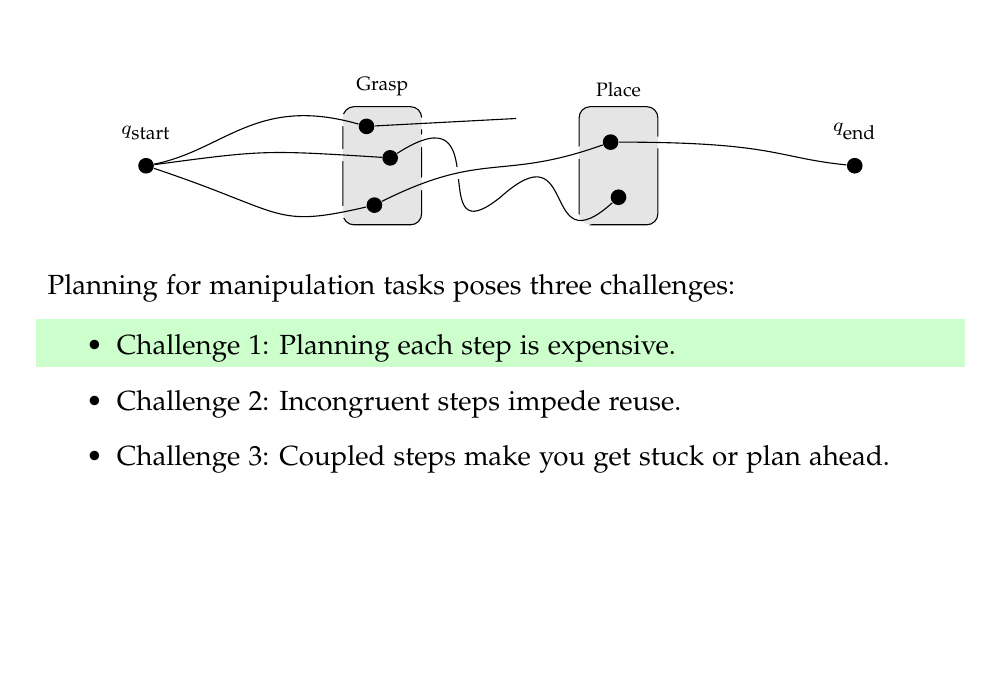
\begin{tikzpicture}
      \draw[step=1,black!10,very thin,opacity=\gridopacity] (0,0) grid (12,8);
   
      % figure adapted from proposal doc
      \begin{scope}[font=\scriptsize,shift={(1.5,6.25)}]
         
         % root sets
         \node[draw,black,rounded corners,minimum height=1.5cm,minimum width=1cm]
            (Xgrasp) at (3,0) {};
         \node[above=0cm of Xgrasp] {Grasp};
         \node[draw,black,rounded corners,minimum height=1.5cm,minimum width=1cm]
            (Xdrop) at (6,0) {};
         \node[above=0cm of Xdrop] {Place};
         
         % nodes
         \node[circle,fill=black,inner sep=2] (xstart) at (0,0) {};
         \node[above=0.1cm of xstart] {$q_{\mbox{\scriptsize start}}$};
         
         % grasp choices
         \node[circle,fill=black,inner sep=2] (xg1) at (2.8,0.5) {};
         \node[circle,fill=black,inner sep=2] (xg2) at (3.1,0.1) {};
         \node[circle,fill=black,inner sep=2] (xg3) at (2.9,-0.5) {};
         % place choices
         \node[circle,fill=black,inner sep=2] (xd1) at (5.9,0.3) {};
         \node[circle,fill=black,inner sep=2] (xd2) at (6.0,-0.4) {};
         % xend 
         \node[circle,fill=black,inner sep=2] (xend) at (9,0) {};
         \node[above=0.1cm of xend] {$q_{\mbox{\scriptsize end}}$};
         
         \draw[line width=1.5mm,white]
            (xstart) .. controls (1,0.2) and (1.4,0.9) .. (xg1);
         \draw[line width=1.5mm,white]
            (xstart) .. controls (1.5,0.2) .. (xg2);
         \draw[line width=1.5mm,white]
            (xstart) .. controls (1.8,-0.6) and (1.6,-0.8) .. (xg3);
         \draw
            (xstart) .. controls (1,0.2) and (1.4,0.9) .. (xg1);
         \draw
            (xstart) .. controls (1.5,0.2) .. (xg2);
         \draw
            (xstart) .. controls (1.8,-0.6) and (1.6,-0.8) .. (xg3);
         \draw[line width=1.5mm,white]
            (xg1) -- (4.7,0.6);
         \draw
            (xg1) -- (4.7,0.6);
         \draw[line width=1.5mm,white]
            (xg2) .. controls (4.5,1) and (3.5,-1.2) .. (4.5,-0.4)
                  .. controls (5.5,0.5) and (5.0,-1.3) .. (xd2);
         \draw
            (xg2) .. controls (4.5,1) and (3.5,-1.2) .. (4.5,-0.4)
                  .. controls (5.5,0.5) and (5.0,-1.3) .. (xd2);
         \draw[line width=1.5mm,white]
            (xg3) .. controls (4.3, 0.2) and (4.5,-0.2) .. (xd1);
         \draw
            (xg3) .. controls (4.3, 0.2) and (4.5,-0.2) .. (xd1);
         % in s3
         \draw[line width=1.5mm,white]
            (xd1) .. controls (8,0.3) and (8,0.1) .. (xend);
         \draw
            (xd1) .. controls (8,0.3) and (8,0.1) .. (xend);
         
         \node[fill,black,rounded corners,minimum height=1.5cm,minimum width=1cm,
            opacity=0.1] at (3,0) {};
         \node[fill,black,rounded corners,minimum height=1.5cm,minimum width=1cm,
            opacity=0.1] at (6,0) {};
         
      \end{scope}
   
      \fill[green!20] (0.1,3.7) rectangle (11.9,4.3);
   
      \node[anchor=north] at (6,5) {\begin{minipage}{11.5cm}
         Planning for manipulation tasks poses three challenges:
         
         \begin{itemize}
         \item Challenge 1: Planning each step is expensive.
         \item Challenge 2: Incongruent steps impede reuse.
         \item Challenge 3: Coupled steps make you get stuck or plan ahead.
         \end{itemize}
      \end{minipage}};
   
   \end{tikzpicture}
\end{frame}


\begin{frame}
   \frametitle{Part 2: Reusing Computation Between Steps}
      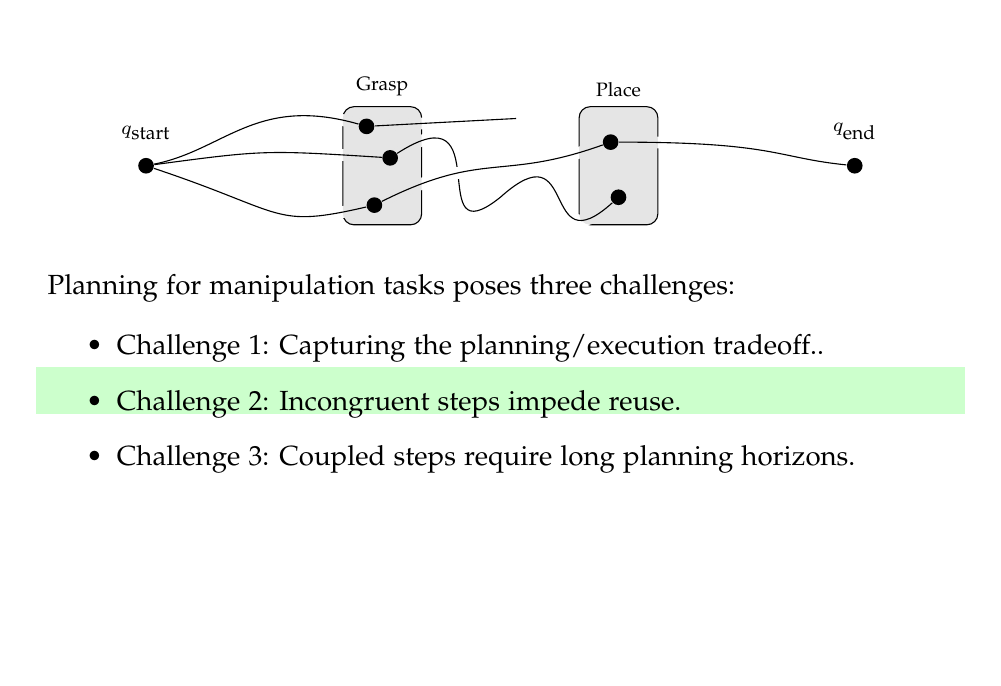
\begin{tikzpicture}
      \draw[step=1,black!15,very thin,opacity=\gridopacity] (0,0) grid (12,8);
   
      % figure adapted from proposal doc
      \begin{scope}[font=\scriptsize,shift={(1.5,6.25)}]
         
         % root sets
         \node[draw,black,rounded corners,minimum height=1.5cm,minimum width=1cm]
            (Xgrasp) at (3,0) {};
         \node[above=0cm of Xgrasp] {Grasp};
         \node[draw,black,rounded corners,minimum height=1.5cm,minimum width=1cm]
            (Xdrop) at (6,0) {};
         \node[above=0cm of Xdrop] {Place};
         
         % nodes
         \node[circle,fill=black,inner sep=2] (xstart) at (0,0) {};
         \node[above=0.1cm of xstart] {$q_{\mbox{\scriptsize start}}$};
         
         % grasp choices
         \node[circle,fill=black,inner sep=2] (xg1) at (2.8,0.5) {};
         \node[circle,fill=black,inner sep=2] (xg2) at (3.1,0.1) {};
         \node[circle,fill=black,inner sep=2] (xg3) at (2.9,-0.5) {};
         % place choices
         \node[circle,fill=black,inner sep=2] (xd1) at (5.9,0.3) {};
         \node[circle,fill=black,inner sep=2] (xd2) at (6.0,-0.4) {};
         % xend 
         \node[circle,fill=black,inner sep=2] (xend) at (9,0) {};
         \node[above=0.1cm of xend] {$q_{\mbox{\scriptsize end}}$};
         
         \draw[line width=1.5mm,white]
            (xstart) .. controls (1,0.2) and (1.4,0.9) .. (xg1);
         \draw[line width=1.5mm,white]
            (xstart) .. controls (1.5,0.2) .. (xg2);
         \draw[line width=1.5mm,white]
            (xstart) .. controls (1.8,-0.6) and (1.6,-0.8) .. (xg3);
         \draw
            (xstart) .. controls (1,0.2) and (1.4,0.9) .. (xg1);
         \draw
            (xstart) .. controls (1.5,0.2) .. (xg2);
         \draw
            (xstart) .. controls (1.8,-0.6) and (1.6,-0.8) .. (xg3);
         \draw[line width=1.5mm,white]
            (xg1) -- (4.7,0.6);
         \draw
            (xg1) -- (4.7,0.6);
         \draw[line width=1.5mm,white]
            (xg2) .. controls (4.5,1) and (3.5,-1.2) .. (4.5,-0.4)
                  .. controls (5.5,0.5) and (5.0,-1.3) .. (xd2);
         \draw
            (xg2) .. controls (4.5,1) and (3.5,-1.2) .. (4.5,-0.4)
                  .. controls (5.5,0.5) and (5.0,-1.3) .. (xd2);
         \draw[line width=1.5mm,white]
            (xg3) .. controls (4.3, 0.2) and (4.5,-0.2) .. (xd1);
         \draw
            (xg3) .. controls (4.3, 0.2) and (4.5,-0.2) .. (xd1);
         % in s3
         \draw[line width=1.5mm,white]
            (xd1) .. controls (8,0.3) and (8,0.1) .. (xend);
         \draw
            (xd1) .. controls (8,0.3) and (8,0.1) .. (xend);
         
         \node[fill,black,rounded corners,minimum height=1.5cm,minimum width=1cm,
            opacity=0.1] at (3,0) {};
         \node[fill,black,rounded corners,minimum height=1.5cm,minimum width=1cm,
            opacity=0.1] at (6,0) {};
         
      \end{scope}
   
      \fill[green!20] (0.1,3.1) rectangle (11.9,3.7);
   
      \node[anchor=north] at (6,5) {\begin{minipage}{11.5cm}
         Planning for manipulation tasks poses three challenges:
         
         \begin{itemize}
         \item Challenge 1: Capturing the planning/execution tradeoff..
         \item Challenge 2: Incongruent steps impede reuse.
         \item Challenge 3: Coupled steps require long planning horizons.
         \end{itemize}
      \end{minipage}};
   
   \end{tikzpicture}
\end{frame}

\begin{frame}
   \frametitle{Motivation: Structure of Manipulation Problems}
   
   \includegraphics[width=\textwidth]{figs/fridge-intro.png}
   
\end{frame}

\begin{frame}
   \frametitle{Motivation: 2D Example}
   \begin{tikzpicture}

      \draw[step=1,black!15,very thin,opacity=\gridopacity] (0,0) grid (12,8);
      
      \node[inner sep=0] at (5.5,4.75) {
         \includegraphics[width=5cm]{figs/alami-intro.png}
      };
      
      \node[inner sep=0pt] at (6,0.5) {\begin{minipage}{7.75cm}\scriptsize{
         $^\dag$\PaperPortrait\;  Alami, Simeon, and Laumond,
         ``A Geometrical Approach to Planning Manipulation Tasks,'' ISRR 1990.
      }\end{minipage}};
      
   \end{tikzpicture}
\end{frame}


\begin{frame}
   \frametitle{Motivation: 2D Example}
   \begin{tikzpicture}
   
      \draw[step=1,black!15,very thin,opacity=\gridopacity] (0,0) grid (12,8);
      
      \node[inner sep=0] at (5.5,6.75) {
         \includegraphics[width=5cm]{figs/alami-intro.png}
      };
      
      \node[inner sep=0] at (0.75,4.25) {\includegraphics[width=1cm]{figs/alami-transit-1.png}};
      \node[inner sep=0] at (0.75,3.6) {\includegraphics[width=1cm]{figs/alami-intersection.png}};
      \node[inner sep=0] at (0.75,2.95) {\includegraphics[width=1cm]{figs/alami-transit-4.png}};
      \node[inner sep=0] at (0.75,2.3) {\includegraphics[width=1cm]{figs/alami-transit-3.png}};
      \node[inner sep=0] at (0.75,1.65) {\includegraphics[width=1cm]{figs/alami-transit-2.png}};
      
      \node at (3.25,4.9) {Transit Slice:};
      \node[inner sep=0] at (3.5,3.5) {%
         \only<1>{\includegraphics[width=4cm]{figs/alami-intersection.png}}%
         \only<2>{\includegraphics[width=4cm]{figs/alami-transit-1.png}}%
         \only<3>{\includegraphics[width=4cm]{figs/alami-intersection.png}}%
         \only<4>{\includegraphics[width=4cm]{figs/alami-transit-4.png}}%
         \only<5>{\includegraphics[width=4cm]{figs/alami-transit-3.png}}%
         \only<6>{\includegraphics[width=4cm]{figs/alami-transit-2.png}}%
         \only<7->{\includegraphics[width=4cm]{figs/alami-intersection.png}}%
      };
      \node[inner sep=0] at (3.5,1.25) {
         \includegraphics[width=4cm]{figs/alami-transit-slice.png}
      };
      
      \node[inner sep=0] at (11.25,4.25) {\includegraphics[width=1cm]{figs/alami-transfer-1.png}};
      \node[inner sep=0] at (11.25,3.6) {\includegraphics[width=1cm]{figs/alami-intersection.png}};
      \node[inner sep=0] at (11.25,2.95) {\includegraphics[width=1cm]{figs/alami-transfer-2.png}};
      
      \node at (8.75,4.9) {Transfer Slice:};
      \node[inner sep=0] at (8.5,3.5) {%
         \only<-7>{\includegraphics[width=4cm]{figs/alami-intersection.png}}%
         \only<8>{\includegraphics[width=4cm]{figs/alami-transfer-1.png}}%
         \only<9>{\includegraphics[width=4cm]{figs/alami-intersection.png}}%
         \only<10>{\includegraphics[width=4cm]{figs/alami-transfer-2.png}}%
         \only<11>{\includegraphics[width=4cm]{figs/alami-intersection.png}}%
      };
      \node[inner sep=0] at (8.5,1.25) {
         \includegraphics[width=4cm]{figs/alami-transfer-slice.png}
      };
      
   \end{tikzpicture}
\end{frame}

\begin{frame}
   \frametitle{Motivation: 2D Example}
   \begin{tikzpicture}
      \draw[step=1,black!15,very thin,opacity=\gridopacity] (0,0) grid (12,8);
      
      \node[inner sep=0pt] at (6,7) {\begin{minipage}{11.5cm}\centering
         After every grasp and release,
         the projection of the current manifold of $\Pi\mathcal{C}$ onto
         $\mathcal{C}_{\ms{R}}$ changes!
      \end{minipage}};

      \node[inner sep=0] at ( 1.50,5.5) {\includegraphics[width=2cm]{figs/alami-slice-01.png}};
      \node[inner sep=0] at ( 3.75,5.5) {\includegraphics[width=2cm]{figs/alami-slice-02.png}};
      \node[inner sep=0] at ( 6.00,5.5) {\includegraphics[width=2cm]{figs/alami-slice-03.png}};
      \node[inner sep=0] at ( 8.25,5.5) {\includegraphics[width=2cm]{figs/alami-slice-04.png}};
      \node[inner sep=0] at (10.50,5.5) {\includegraphics[width=2cm]{figs/alami-slice-05.png}};
      \node[inner sep=0] at ( 1.50,4.0) {\includegraphics[width=2cm]{figs/alami-slice-06.png}};
      \node[inner sep=0] at ( 3.75,4.0) {\includegraphics[width=2cm]{figs/alami-slice-07.png}};
      \node[inner sep=0] at ( 6.00,4.0) {\includegraphics[width=2cm]{figs/alami-slice-08.png}};
      \node[inner sep=0] at ( 8.25,4.0) {\includegraphics[width=2cm]{figs/alami-slice-09.png}};
      \node[inner sep=0] at (10.50,4.0) {\includegraphics[width=2cm]{figs/alami-slice-10.png}};

      \node[inner sep=0pt] at (6,2.5) {\begin{minipage}{11.5cm}\centering
         Do we need to build a separate roadmap in each slice?
      \end{minipage}};

   \end{tikzpicture}
\end{frame}

\begin{frame}
   \frametitle{Manipulation Example}
   \begin{tikzpicture}
      \draw[step=1,black!15,very thin,opacity=\gridopacity] (0,0) grid (12,8);
      
      \node at (3,6.5) {\includegraphics[width=4.5cm]{build/example-2d-q1}};
      
      \only<3->{
         \node[inner sep=0pt] at (9,7) {\begin{minipage}{5.5cm}\centering
            Query C-Space Subsets:
            
            $S_{12} \subseteq \mathcal{C}$
            
            $S_{23} \subseteq \mathcal{C}$
         \end{minipage}};
      }
      
      \only<3>{
         \node at (9,5.25) {\includegraphics[width=4.5cm]{build/example-2d-s12}};
      }
      \only<4->{
         \node at (9,5.25) {\includegraphics[width=4.5cm]{build/example-2d-s12-wtraj}};
      }
      
      \only<5->{
         \node at (3,4) {\includegraphics[width=4.5cm]{build/example-2d-b}};
      }
      
      \only<6>{
         \node at (9,2.75) {\includegraphics[width=4.5cm]{build/example-2d-s23}};
      }
      \only<7->{
         \node at (9,2.75) {\includegraphics[width=4.5cm]{build/example-2d-s23-wtraj}};
      }
      
      \only<2->{
         \node at (3,1.5) {\includegraphics[width=4.5cm]{build/example-2d-q3}};
      }

   \end{tikzpicture}
\end{frame}

\begin{frame}
   \frametitle{Manipulation Example}
   \begin{tikzpicture}
      \draw[step=1,black!15,very thin,opacity=\gridopacity] (0,0) grid (12,8);
      
      \node at (3,6.5) {\includegraphics[width=4.5cm]{build/example-2d-q1}};
      \node at (3,4) {\includegraphics[width=4.5cm]{build/example-2d-b}};
      \node at (3,1.5) {\includegraphics[width=4.5cm]{build/example-2d-q3}};
      
      \node at (9,4) {\includegraphics{build/figstar-a-qlabeled}};
      
   \end{tikzpicture}
\end{frame}

\begin{frame}
   \frametitle{Workspace Decompositions to C-Space Relations}
   \begin{tikzpicture}
      \draw[step=1,black!15,very thin,opacity=\gridopacity] (0,0) grid (12,8);

      \node[draw,align=center] at (2,6.75) {Workspace\\obstacle\\$W_X$};
      \draw[->,line width=1pt] (3.25,6.75) -- (4.25,6.75);
      \node[align=center] at (6,6.75) {C-Space\\Transforms};
      \draw[->,line width=1pt] (7.75,6.75) -- (8.75,6.75);
      \node[draw,align=center] at (10,6.75) {Valid (free)\\$\mathcal{C}$-subset\\$S_X$};

      % procedure itself
      \only<2->{
         \node[fill=blue!20,rounded corners,anchor=north] at (6,5.5) {\begin{minipage}{5cm}\small{
            {\bf C-Space Set Union Property}$^\dag$
            
            {\bf If} $W_A = W_B \cup W_C$,
            
            {\bf Then} $S_A = S_B \cap S_C$.
         }\end{minipage}};
      
         \node[inner sep=0pt] at (6,0.5) {\begin{minipage}{10.5cm}\scriptsize{
            $^\dag$\PaperPortrait\;  W. S. Newman and M. S. Branicky.
            ``Real-time configuration space transforms for obstacle avoidance.''
            The International Journal of Robotics Research, 1991.
         }\end{minipage}};
      }
      
      \only<3->{
         \node[fill=blue!20,rounded corners,anchor=north] at (6,3.5) {\begin{minipage}{7cm}\small{
            {\bf Example Workspace Decomposition}
            
            {\bf Given} $W_{12}$ {\bf and} $W_{23}$,
            
            {\bf Compute any} $W_C \subseteq W_{12} \cap W_{23}$
            
            {\bf Let} $W_A = W_{12} \setminus W_I$ {\bf and} $W_B = W_{23} \setminus W_I$
            
            {\bf Then} $S_{12} = S_C \cap S_A$ {\bf and} $S_{23} = S_C \cap S_B$
            
         }\end{minipage}};
      }

   \end{tikzpicture}
\end{frame}

\begin{frame}
   \frametitle{Manipulation Example}
   \begin{tikzpicture}
      \draw[step=1,black!15,very thin,opacity=\gridopacity] (0,0) grid (12,8);
      
      \node[font=\small,anchor=east] at (5.25,6.25) {${\hat p}_{12}(q) = 6$};
      \node at (3,5.25) {\includegraphics[width=4.5cm]{build/example-2d-s12}};
      \node[font=\small,anchor=east] at (5.25,3.75) {${\hat p}_{23}(q) = 6$};
      \node at (3,2.75) {\includegraphics[width=4.5cm]{build/example-2d-s23}};
      
      
      \only<3->{
         \node[font=\small,anchor=east] at (11.25,7.5) {${\hat p}_A(q) = 2$};
         \node at (9,6.5) {\includegraphics[width=4.5cm]{build/example-2d-sa}};
      }
      \only<2->{
         \node[font=\small,anchor=east] at (11.25,5.0) {${\hat p}_C(q) = 4$};
         \node at (9,4.0) {\includegraphics[width=4.5cm]{build/example-2d-sc}};
      }
      \only<4->{
         \node[font=\small,anchor=east] at (11.25,2.5) {${\hat p}_B(q) = 2$};
         \node at (9,1.5) {\includegraphics[width=4.5cm]{build/example-2d-sb}};
      }
      
   \end{tikzpicture}
\end{frame}

\begin{frame}
   \frametitle{Manipulation Example}
   \begin{tikzpicture}
      \draw[step=1,black!15,very thin,opacity=\gridopacity] (0,0) grid (12,8);

      \only<1-2>{\node at (9,3.5) {\includegraphics{build/figstar-wo-abc}};}
      
      % left
      \only<1>{
         \node[font=\small,anchor=east] at (5.25,6.25) {${\hat p}_{12}(q) = 6$};
         \node at (3,5.25) {\includegraphics[width=4.5cm]{build/example-2d-s12}};
         \node[font=\small,anchor=east] at (5.25,3.75) {${\hat p}_{23}(q) = 6$};
         \node at (3,2.75) {\includegraphics[width=4.5cm]{build/example-2d-s23}};
      }
      \only<2-3>{
      
         \node[inner sep=0pt] at (3,7.35) {\begin{minipage}{6cm}\centering\small
            $W_{12} = W_C \cup W_A$
            
            $W_{23} = W_C \cup W_B$
         \end{minipage}};
      
         \node[font=\small,anchor=east] at (5.25,6.50) {${\hat p}_A(q) = 2$};
         \node at (3,5.50) {\includegraphics[width=4.5cm]{build/example-2d-sa}};
         \node[font=\small,anchor=east] at (5.25,4.25) {${\hat p}_C(q) = 4$};
         \node at (3,3.25) {\includegraphics[width=4.5cm]{build/example-2d-sc}};
         \node[font=\small,anchor=east] at (5.25,2.00) {${\hat p}_B(q) = 2$};
         \node at (3,1.00) {\includegraphics[width=4.5cm]{build/example-2d-sb}};
      }
      
      % right
      \only<3->{
         \node[inner sep=0pt] at (9,6.75) {\begin{minipage}{6cm}\centering\small
            $S_{12} = S_C \cap S_A$
            
            $S_{23} = S_C \cap S_B$
         \end{minipage}};
      
         \only<3>{\node at (9,3.5) {\includegraphics{build/figstar-w-abc}};}
         \only<4>{\node at (9,3.5) {\includegraphics{build/figstar-traj1}};}
         \only<5>{\node at (9,3.5) {\includegraphics{build/figstar-traj1-inc}};}
      }
      
      % left again
      \only<4->{
         \node at (3,5.25) {\includegraphics[width=4.5cm]{build/example-2d-s12-wtraj}};
      }
      \only<5->{
         \node at (3,2.75) {\includegraphics[width=4.5cm]{build/example-2d-s23-wtraj}};
      }
      
   \end{tikzpicture}
\end{frame}

\begin{frame}
   \frametitle{Multi-Set Planning Formulation}
   \begin{tikzpicture}
      \draw[step=1,black!15,very thin,opacity=\gridopacity] (0,0) grid (12,8);

      % right side
      \node[inner sep=0pt] at (9,6.75) {\begin{minipage}{6cm}\centering\small
            $S_{12} = S_C \cap S_A$
            
            $S_{23} = S_C \cap S_B$
         \end{minipage}};
      \node at (9,3.5) {\includegraphics{build/figstar-w-abc}};
      
      \node[fill=blue!20,rounded corners] at (3,5.5)
      {\begin{minipage}{5cm}
         {\setlength{\tabcolsep}{2pt}
         \begin{tabular}{ccl}
         $\mathcal{C}$ &:& common C-space \\
         \noalign{\medskip}
         $\mathcal{F}$ &:& family of subsets over $\mathcal{C}$ \\
         & & that is, $S \subseteq \mathcal{C} \;\forall\; S \in \mathcal{F}$ \\
         \noalign{\medskip}
         $\mathcal{R}$ &:& set of subset relations \\
         & & e.g. $S_A = S_B \cap S_C$ \\
         \noalign{\medskip}
         $\mathcal{U}$ &:& set of planning queries \\
         & & e.g. $u = (q_{\ms{init}}, q_{\ms{goal}}, S_u)$ \\
         \end{tabular}}
      \end{minipage}};
      
      \node[fill=blue!20,rounded corners] at (3,2)
      {\begin{minipage}{5cm}
         Validity checking model:
         
         {\setlength{\tabcolsep}{2pt}
         \begin{tabular}{ccl}
         ${\bf 1}_A(\cdot)$ &:& indicator for $S_A$ \\
         $p_A(\cdot)$ &:& cost to evaluate ${\bf 1}_A(\cdot)$ \\
         \end{tabular}}
      \end{minipage}};
      
   \end{tikzpicture}
\end{frame}

\begin{frame}
   \frametitle{Instances of Multi-Set Problems in Manipulation}
   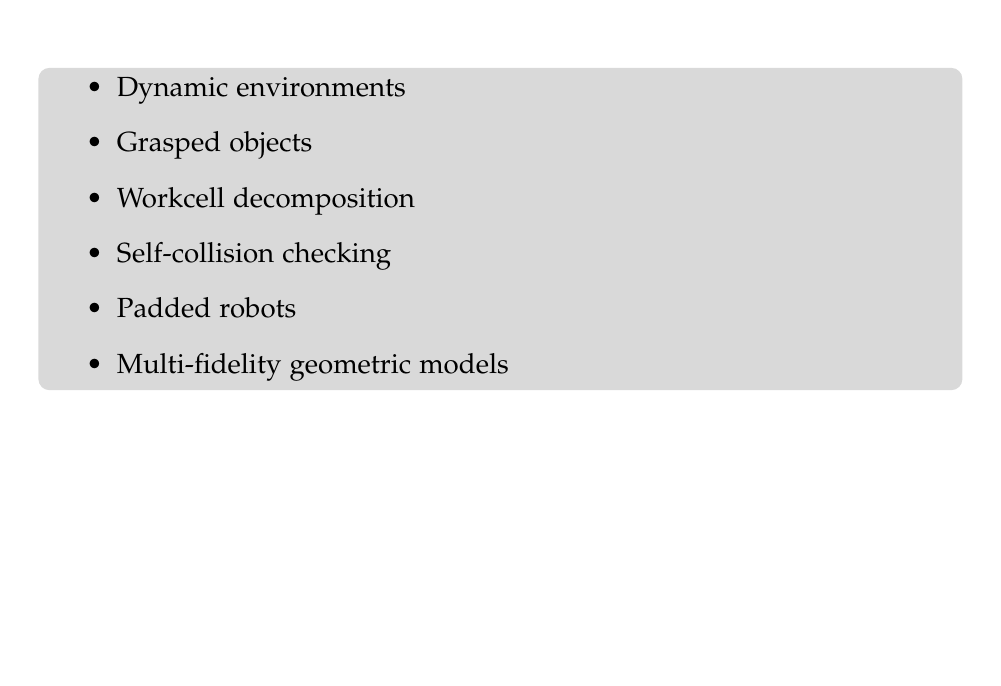
\begin{tikzpicture}
      \draw[step=1,black!15,very thin,opacity=\gridopacity] (0,0) grid (12,8);
      
      \node[anchor=north,fill=black!15,rounded corners]
      at (6,7.5) {\begin{minipage}{11.5cm}
         \begin{itemize}
         \item Dynamic environments
         \item Grasped objects
         \item Workcell decomposition
         \item Self-collision checking
         \item Padded robots
         \item Multi-fidelity geometric models
         \end{itemize}
      \end{minipage}};
   \end{tikzpicture}
\end{frame}

\begin{frame}
   \frametitle{Multi-Set Instances: Dynamic Environments}
   \begin{tikzpicture}
      \draw[step=1,black!15,very thin,opacity=\gridopacity] (0,0) grid (12,8);
      
      \node[inner sep=0pt] at (2.8,4) {%
         \only<1>{\includegraphics[height=7.5cm]{figs/herb-fridge-sets-b.png}}%
         \only<2>{\includegraphics[height=7.5cm]{figs/herb-fridge-sets-a.png}}%
         \only<3>{\includegraphics[height=7.5cm]{figs/herb-fridge-sets-b.png}}%
      };
      
      \node[anchor=north,fill=black!15,rounded corners,font=\small]
      at (8.8,7.75) {\begin{minipage}{6cm}
         The valid set $S_A$ in the presence of an object
         is a subset of the valid set $S_N$ with the object removed.
      \end{minipage}};
      
      \node[inner sep=0pt] at (8.8,4) {%
         \only<1>{\includegraphics[width=4.5cm]{build/multiset-manip-instances,dyna}}%
         \only<2>{\includegraphics[width=4.5cm]{build/multiset-manip-instances,dynb}}%
         \only<3>{\includegraphics[width=4.5cm]{build/multiset-manip-instances,dync}}%
      };
      
   \end{tikzpicture}
\end{frame}

\begin{frame}
   \frametitle{Multi-Set Instances: Dynamic Environments}
   \begin{tikzpicture}
      \draw[step=1,black!15,very thin,opacity=\gridopacity] (0,0) grid (12,8);
      
      \begin{scope}[shift={(1,1.2)},font=\small]
         \node[anchor=south west,inner sep=0] at (0,0)
           {\includegraphics[width=5.2cm]{figs/chimp-voxels-delta.png}};

         \node[draw,inner sep=3pt,fill=white,fill opacity=0.9,align=center]
           (debrislab) at (0.7,1.0) {Debris object\\removed};
         \node[circle,inner sep=2,draw,fill=white] (debris) at (2.2,2.9) {};
         \draw[draw=black, double=white, double distance=1pt, line width=1pt]
           (debrislab.north) -- (debris);
           
         \node[draw,inner sep=3pt,fill=white,fill opacity=0.9,align=center]
           (addlab) at (5.0,2.0) {Additional\\voxels seen};
         \node[circle,inner sep=2,draw,fill=white] (added) at (4.4,5.0) {};
         \draw[draw=black, double=white, double distance=1pt, line width=1pt]
           (addlab.north) -- (added);
      \end{scope}
      
      \node[inner sep=0pt] at (9.5,6) {
         \includegraphics{build/retroactive-a}
      };
      
      \node[inner sep=0pt] at (9.5,2) {
         \includegraphics{build/retroactive-b}
      };
   \end{tikzpicture}
\end{frame}

\begin{frame}
   \frametitle{Multi-Set Instances: Grasped Objects}
   \begin{tikzpicture}
      \draw[step=1,black!15,very thin,opacity=\gridopacity] (0,0) grid (12,8);
      
      \node[inner sep=0pt] at (2.8,4) {%
         \only<1>{\includegraphics[height=7.5cm]{figs/herb-fridge-sets-c.png}}%
         \only<2>{\includegraphics[height=7.5cm]{figs/herb-fridge-sets-a.png}}%
         \only<3>{\includegraphics[height=7.5cm]{figs/herb-fridge-sets-c.png}}%
      };
      
      \node[anchor=north,fill=black!15,rounded corners,font=\small]
      at (8.8,7.75) {\begin{minipage}{6cm}
         The valid set $S_A$ while grasping an object
         is a subset of the valid set $S_N$ with the object removed.
      \end{minipage}};
      
      \node[inner sep=0pt] at (8.8,4) {%
         \only<1>{\includegraphics[width=4.5cm]{build/multiset-manip-instances,dyna}}%
         \only<2>{\includegraphics[width=4.5cm]{build/multiset-manip-instances,dynb}}%
         \only<3>{\includegraphics[width=4.5cm]{build/multiset-manip-instances,dync}}%
      };
      
   \end{tikzpicture}
\end{frame}

\begin{frame}
   \frametitle{Multi-Set Instances: Self-Collision Checking}
   \begin{tikzpicture}
      \draw[step=1,black!15,very thin,opacity=\gridopacity] (0,0) grid (12,8);

      \node[inner sep=0pt] at (2.8,4) {%
         \only<1>{\includegraphics[height=7.5cm]{figs/herb-fridge-sets-a.png}}%
         \only<2>{\includegraphics[height=7.5cm]{figs/herb-fridge-sets-d.png}}%
         \only<3>{\includegraphics[height=7.5cm]{figs/herb-fridge-sets-a.png}}%
      };

      \node[anchor=north,fill=black!15,rounded corners,font=\small]
      at (8.8,7.75) {\begin{minipage}{6cm}
         The valid set $S_A$
         is a subset of the valid set $S_R$
         consisting of robot self-collision-free configurations.
      \end{minipage}};

      \node[inner sep=0pt] at (8.8,4) {%
         \only<1>{\includegraphics[width=4.5cm]{build/multiset-manip-instances,selfa}}%
         \only<2>{\includegraphics[width=4.5cm]{build/multiset-manip-instances,selfb}}%
         \only<3>{\includegraphics[width=4.5cm]{build/multiset-manip-instances,selfc}}%
      };

   \end{tikzpicture}
\end{frame}

\begin{frame}
   \frametitle{Multi-Set Instances: Conservative Obstacle Volumes}
   \begin{tikzpicture}
      \draw[step=1,black!15,very thin,opacity=\gridopacity] (0,0) grid (12,8);
      
      \node[inner sep=0pt] at (2.8,4) {%
         \only<1>{\includegraphics[height=7.5cm]{figs/herb-fridge-sets-h.png}}%
         \only<2-3>{\includegraphics[height=7.5cm]{figs/herb-fridge-sets-e.png}}%
      };
      
      \node[anchor=north,fill=black!15,rounded corners,font=\small]
      at (8.8,7.75) {\begin{minipage}{6cm}
         The valid set $S_O$ in the presence of an object
         can be conservatively bounded by a simpler geometry
         yielding $S_B$.
      \end{minipage}};
      
      \node[inner sep=0pt] at (8.8,4) {%
         \only<1>{\includegraphics[width=4.5cm]{build/multiset-manip-instances-blob,outside}}%
         \only<2->{\includegraphics[width=4.5cm]{build/multiset-manip-instances-blob,inside}}%
      };
      
      \only<3->{
         \node[anchor=north,fill=black!15,rounded corners,font=\small]
         at (8.8,2) {\begin{minipage}{6cm}
            Extreme case: Leven/Hutchinson workcell decomposition.
         \end{minipage}};
      }
      
   \end{tikzpicture}
\end{frame}

\begin{frame}
   \frametitle{Multi-Set Instances: Conservative Grasped Volumes}
   \begin{tikzpicture}
      \draw[step=1,black!15,very thin,opacity=\gridopacity] (0,0) grid (12,8);
      
      \node[inner sep=0pt] at (2.8,4) {%
         \only<1>{\includegraphics[height=7.5cm]{figs/herb-fridge-sets-c.png}}%
         \only<2>{\includegraphics[height=7.5cm]{figs/herb-fridge-sets-i.png}}%
      };
      
      \node[anchor=north,fill=black!15,rounded corners,font=\small]
      at (8.8,7.75) {\begin{minipage}{6cm}
         The valid set $S_O$ while grabbing the object
         can be conservatively bounded by a simpler geometry
         yielding $S_B$.
      \end{minipage}};
      
      \node[inner sep=0pt] at (8.8,4) {%
         \only<1>{\includegraphics[width=4.5cm]{build/multiset-manip-instances-blob,outside}}%
         \only<2>{\includegraphics[width=4.5cm]{build/multiset-manip-instances-blob,inside}}%
      };

   \end{tikzpicture}
\end{frame}

\begin{frame}
   \frametitle{Multi-Set Instances: Conservative Robot Models}
   \begin{tikzpicture}
      \draw[step=1,black!15,very thin,opacity=\gridopacity] (0,0) grid (12,8);
      
      \node[inner sep=0pt] at (2.8,4) {%
         \only<1>{\includegraphics[height=7.5cm]{figs/herb-fridge-sets-j.png}}%
         \only<2->{\includegraphics[height=7.5cm]{figs/herb-fridge-sets-k.png}}%
      };
      
      \node[anchor=north,fill=black!15,rounded corners,font=\small]
      at (8.8,7.75) {\begin{minipage}{6cm}
         The valid set $S_R$ while grabbing the object
         can be conservatively bounded by a simpler geometry
         yielding $S_B$.
      \end{minipage}};
      
      \node[inner sep=0pt] at (8.8,4) {%
         \only<1>{\includegraphics[width=4.5cm]{build/multiset-manip-instances-blob,routside}}%
         \only<2>{\includegraphics[width=4.5cm]{build/multiset-manip-instances-blob,rinside}}%
      };
   
   \end{tikzpicture}
\end{frame}

\begin{frame}
   \frametitle{Instances of Multi-Set Problems in Manipulation}
   \begin{tikzpicture}
      \draw[step=1,black!15,very thin,opacity=\gridopacity] (0,0) grid (12,8);
      
      \node[anchor=north,fill=black!15,rounded corners]
      at (6,7.5) {\begin{minipage}{11.5cm}
         \begin{itemize}
         \item Dynamic environments
         \item Grasped objects
         \item Workcell decomposition
         \item Self-collision checking
         \item Padded robots
         \item Multi-fidelity geometric models
         \end{itemize}
      \end{minipage}};
      
      \only<2->{
         \node[fill=blue!20,rounded corners,anchor=north]
         at (6,3.5) {\begin{minipage}{9.5cm}
            {\bf Research Question Q3:}
            
            \smallskip
            Perform a comprehensive literature survey to identify
            and classify instances of multi-set motion planning.
            
            \smallskip
            Also characterize other approaches to caching and
            relating similar problems that cannot be represented
            as a multi-set problem.
         \end{minipage}};
      }
      
   \end{tikzpicture}
\end{frame}

\begin{frame}
   \frametitle{Applying the E$^8$-PRM to the Multi-Set Problem}
   \begin{tikzpicture}
      \draw[step=1,black!15,very thin,opacity=\gridopacity] (0,0) grid (12,8);

      \node[fill=blue!20,align=center,rounded corners,
         inner sep=5pt] at (1.5,5.3) {
         Propositional\\
         Logic Solver
      };
      
      \draw[<->,line width=1pt] (2.8,5.3) -- (3.3,5.3);

      \node[shape=document,draw,inner sep=0.25cm,align=center,
         font=\small,anchor=south] at (5,4.5) {
         Multi-Set\\
         ensemble effort\\
         model $\mathcal{M}_{\ms{multi}}$};
      
      \node[anchor=south,shape=document,draw,align=center]
      at (9,4.5) {
         Graph G\\
         \includegraphics[width=2.5cm]{build/roadmap-2d-simple}
         %\includegraphics[width=2.5cm]{build/talk-act1-2d,graph}
         
      };
      
      \draw[->,line width=1pt] (6.3,4.4) -- (6.3,3.9);
      \draw[->,line width=1pt] (7.8,4.4) -- (7.8,3.9);
      
      \node[fill=blue!20,minimum height=1.5cm,minimum width=2.5cm,
         align=center,rounded corners,inner ysep=0.7cm]
      at (7,2.5) {
         E$^8$-PRM\\
         \small{$\min
         \left[ (1 - \lambda) \hat{f}_x + \lambda \hat{f}_p \right]$}
      };
      
      \node[shape=document,draw,align=center,inner xsep=10pt]
      at (2.4,3) {
         Query $V_{s1}$, $V_{g1}$, $\lambda_1$
      };
      \draw[->,line width=1pt] (4.5,3) -- (5.0,3);
      
      \draw[->,line width=1pt] (9,3) -- (9.5,3);
      \node[shape=document,draw,align=center,inner xsep=5pt]
      at (10.1,3) {$\pi^*_1$\;\;};
      
      \node[shape=document,draw,align=center,inner xsep=10pt]
      at (2.4,2) {
         Query $V_{s2}$, $V_{g2}$, $\lambda_2$
      };
      \draw[->,line width=1pt] (4.5,2) -- (5.0,2);
      
      \draw[->,line width=1pt] (9,2) -- (9.5,2);
      \node[shape=document,draw,align=center,inner xsep=5pt]
      at (10.1,2) {$\pi^*_2$\;\;};

      \node[inner sep=0pt] at (6,0.5) {\begin{minipage}{11.5cm}\centering
         This is the Multi-Set PRM.
      \end{minipage}};

   \end{tikzpicture}
\end{frame}

\begin{frame}
   \frametitle{Multi-Set Reasoning with Propositional Logic}
   \begin{tikzpicture}
      \draw[step=1,black!15,very thin,opacity=\gridopacity] (0,0) grid (12,8);

      \node[inner sep=0pt] at (5,6.15) {%
         \only<1>{\includegraphics[width=4.5cm]{build/multiset-roadmap-example,start}}%
         \only<2>{\includegraphics[width=4.5cm]{build/multiset-roadmap-example,roadmap}}%
         \only<3>{\includegraphics[width=4.5cm]{build/multiset-roadmap-example,straightsol}}%
         \only<4-5>{\includegraphics[width=4.5cm]{build/multiset-roadmap-example,basesets}}%
         \only<6>{\includegraphics[width=4.5cm]{build/multiset-roadmap-example,blackgraph}}%
         \only<7>{\includegraphics[width=4.5cm]{build/multiset-roadmap-example,rightsol}}%
         \only<8>{\includegraphics[width=4.5cm]{build/multiset-roadmap-example,leftspec}}%
         \only<9>{\includegraphics[width=4.5cm]{build/multiset-roadmap-example,leftsol}}%
      };
      
      \node[font=\scriptsize,anchor=west] at (7.7,7) {%
         ${\hat p}_u = 2$%
         \only<5->{, \; ${\hat p}_A = {\hat p}_B = 1$}
      };
      
      \only<2->{
         \draw[dotted] (7.7,6.5) -- (8.2,6.5);
         \fill (7.7,6.5) circle (0.04cm);
         \fill (8.2,6.5) circle (0.04cm);
         \node[font=\scriptsize,anchor=west] at (8.3,6.5) {unknown};
      }
      
      \only<3->{
         \draw[color=black!20,line width=5,line cap=round] (7.7,6) -- (8.2,6);
         \node[font=\scriptsize,anchor=west] at (8.3,6) {candidate path ${\hat \pi}^*$};
      }
      
      \only<4->{
         \node[font=\scriptsize,anchor=west] at (7.7,5.5) {$S_u = S_A \cap S_B$};
      }
      
      \only<6->{
         \draw (7.7,5) -- (8.2,5);
         \fill (7.7,5) circle (0.04cm);
         \fill (8.2,5) circle (0.04cm);
         \node[font=\scriptsize,anchor=west] at (8.3,5) {known in $S_A$};
      }
      
      \node[fill=blue!20,rounded corners,font=\scriptsize] at (5,2.1)
      {\begin{minipage}{8cm}
         \begin{algorithmic}[1]
         \Function {MultiOptCert}{$q_e, S_u, P_{\ms{known}}$}
            \State $\mathcal{T}_{\ms{imply}} \leftarrow \emptyset$
            \ForAll {$\mathcal{F}_{\ms{cert}} \in \mathcal{P}(\mathcal{F})$}
                  \label{line:power-set}
               \State ${\hat p}_{\ms{cert}} \leftarrow \sum_{S \in \mathcal{F}_{\ms{cert}}} \hat{p}_S[q_e]$
               \ForAll {$b_{\ms{res}} \mbox{ \textbf{s.t.} }
                     b_{\ms{res}} : \mathcal{F}_{\ms{cert}} \rightarrow \{\mbox{True},\mbox{False}\}$}
                     \label{line:all-binary-functions}
                  \State $\arraycolsep=2pt
                     P_{\ms{res}} \leftarrow
                     \left\{\left. \begin{array}{rl}
                     \mathbf{1}_S & \mbox{if } b_{\ms{res}}(S) \\
                     \lnot \mathbf{1}_S & \mbox{otherwise} \\
                     \end{array}
                     \right|
                     S \in \mathcal{F}_{\ms{cert}}
                     \right\}$
                  \If {$P_{\ms{known}} \cup P_{\ms{res}}
                        \Rightarrow \mathbf{1}_u$ is valid}
                     \State $\mathcal{T}_{\ms{imply}} \leftarrow
                        \mathcal{T}_{\ms{imply}} \cup
                        \{ (\mathcal{F}_{\ms{cert}}, b_{\ms{res}}, {\hat p}_{\ms{cert}}) \}$
                  \EndIf
               \EndFor
            \EndFor
            \State \Return $(\mathcal{F}_{\ms{cert}}, b_{\ms{res}}, {\hat p}_{\ms{cert}})
               \in \mathcal{T}_{\ms{imply}}$
               with lowest ${\hat p}_{\ms{cert}}$
         \EndFunction
         \end{algorithmic}
      \end{minipage}};
      
      \draw[->,line width=1pt] (9.3,2.1) -- (9.8,2.1);
      \node[draw,shape=document,align=center,font=\scriptsize,minimum height=2cm]
         at (10.9,2.1) {Optimistic\\Edge\\Certificate};
      
   \end{tikzpicture}
\end{frame}

\begin{frame}
   \frametitle{Multi-Set PRM Complexity in the Number of Subsets}
   \begin{tikzpicture}
      \draw[step=1,black!15,very thin,opacity=\gridopacity] (0,0) grid (12,8);
   
      \node[fill=blue!20,rounded corners,font=\scriptsize] at (5,5.6)
      {\begin{minipage}{8cm}
         \begin{algorithmic}[1]
         \Function {MultiOptCert}{$q_e, S_u, P_{\ms{known}}$}
            \State $\mathcal{T}_{\ms{imply}} \leftarrow \emptyset$
            \ForAll {$\mathcal{F}_{\ms{cert}} \in \mathcal{P}(\mathcal{F})$}
                  \label{line:power-set}
               \State ${\hat p}_{\ms{cert}} \leftarrow \sum_{S \in \mathcal{F}_{\ms{cert}}} \hat{p}_S[q_e]$
               \ForAll {$b_{\ms{res}} \mbox{ \textbf{s.t.} }
                     b_{\ms{res}} : \mathcal{F}_{\ms{cert}} \rightarrow \{\mbox{True},\mbox{False}\}$}
                     \label{line:all-binary-functions}
                  \State $\arraycolsep=2pt
                     P_{\ms{res}} \leftarrow
                     \left\{\left. \begin{array}{rl}
                     \mathbf{1}_S & \mbox{if } b_{\ms{res}}(S) \\
                     \lnot \mathbf{1}_S & \mbox{otherwise} \\
                     \end{array}
                     \right|
                     S \in \mathcal{F}_{\ms{cert}}
                     \right\}$
                  \If {$P_{\ms{known}} \cup P_{\ms{res}}
                        \Rightarrow \mathbf{1}_u$ is valid}
                     \State $\mathcal{T}_{\ms{imply}} \leftarrow
                        \mathcal{T}_{\ms{imply}} \cup
                        \{ (\mathcal{F}_{\ms{cert}}, b_{\ms{res}}, {\hat p}_{\ms{cert}}) \}$
                  \EndIf
               \EndFor
            \EndFor
            \State \Return $(\mathcal{F}_{\ms{cert}}, b_{\ms{res}}, {\hat p}_{\ms{cert}})
               \in \mathcal{T}_{\ms{imply}}$
               with lowest ${\hat p}_{\ms{cert}}$
         \EndFunction
         \end{algorithmic}
      \end{minipage}};
      
      \draw[->,line width=1pt] (9.3,5.5) -- (9.8,5.5);
      \node[draw,shape=document,align=center,font=\scriptsize,minimum height=2cm]
         at (10.9,5.5) {Optimistic\\Edge\\Certificate};
   
      \only<2->{
         \node[fill=blue!20,rounded corners,anchor=north]
         at (6,3.2) {\begin{minipage}{10.5cm}
            {\bf Research Question Q4:}
            
            \smallskip
            How should the planner manage the potential explosion
            of known subsets over its lifetime?
            
            \smallskip
            Ideas: limiting roadmap depth,
            periodically force-evaluating and/or pruning old subsets
            
         \end{minipage}};
      }
   
   %Talk about failure modes!
   %This is a research question.
   %Complexity, triple-exponential in number of sets?
   
   \end{tikzpicture}
\end{frame}

\begin{frame}
   \frametitle{Multi-Set PRM Behavior: Conservative Volumes}
   \begin{tikzpicture}
      \draw[step=1,black!15,very thin,opacity=\gridopacity] (0,0) grid (12,8);
   
      \node[draw,color=black!25,inner sep=1pt] (lambda0) at (3,6) {%
         \only<1>{\includegraphics[width=5cm]{figs/bean-allpaths-lambda0.png}}%
         \only<2-3>{\includegraphics[width=5cm]{figs/bean-allpaths-padded-lambda0.png}}%
      };
      \node[font=\small,below left=0cm of lambda0.north east] {$\lambda = 0$};
      
      \node[draw,color=black!25,inner sep=1pt] (lambda1) at (3,2) {%
         \only<1-2>{\includegraphics[width=5cm]{figs/bean-allpaths-lambda1.png}}%
         \only<3>{\includegraphics[width=5cm]{figs/bean-allpaths-padded-lambda1.png}}%
      };
      \node[font=\small,below left=0cm of lambda1.north east] {$\lambda = 1$};
      
      \begin{scope}[shift={(7.5,2.5)},font=\small]
      \begin{axis}[
         xlabel=Collision Checks,
         ylabel=Path Length,
         ylabel near ticks,
         xlabel near ticks,
         scaled x ticks=base 10:-3,
         scaled y ticks=base 10:-2,
         every x tick scale label/.style={
            at={(1,-0.2075)}
         },
         %ticks=none,
         axis lines=left,
         xmin=0,xmax=8000,
         ymin=700,ymax=950,
         width=5.5cm, height=5.5cm]
      
      \coordinate (l0) at (axis cs:7219.5, 733.0);
      \coordinate (l1) at (axis cs:4692.6, 836.5);
      \coordinate (l0pad) at (axis cs:2685.7, 733.0);
      \coordinate (l1pad) at (axis cs:1064.5, 907.1);

      \addplot[mark=*] plot coordinates { (7219.5, 733.0) };
      \addplot[mark=*] plot coordinates { (4692.6, 836.5) };

      \node (labl0) at ($ (l0) + (-10,20) $) {$\lambda=0$};
      \node (labl1) at ($ (l1) + (70,20) $) {$\lambda=1$};
      %\draw[->] (labl0) -- ($ (l0)!0.25cm!(labl0) $);
      %\draw[->] (labl1) -- ($ (l1)!0.25cm!(labl1) $);

      % padded nodes
      \only<2-3>{
         \addplot[mark=*] plot coordinates { (2685.7, 733.0) };
         \draw[->,line width=1pt] ($ (l0)!0.15cm!(l0pad) $) -- ($ (l0pad)!0.15cm!(l0) $);
      }
      \only<3>{
         \addplot[mark=*] plot coordinates { (1064.5, 907.1) };
         \draw[->,line width=1pt] ($ (l1)!0.15cm!(l1pad) $) -- ($ (l1pad)!0.15cm!(l1) $);
      }
      
      \end{axis}
      \end{scope}
   
   \end{tikzpicture}
\end{frame}

\begin{frame}
   \frametitle{HERB Example Problem}
   \begin{tikzpicture}
      \draw[step=1,black!15,very thin,opacity=\gridopacity] (0,0) grid (12,8);
   
      \node[inner sep=0pt]
         at ( 1.50,6.6) {\includegraphics[width=2cm]{figs/testherb-a.png}};
      \node[inner sep=0pt]
         at ( 3.75,6.6) {\includegraphics[width=2cm]{figs/testherb-b.png}};
      \node[inner sep=0pt]
         at ( 6.00,6.6) {\includegraphics[width=2cm]{figs/testherb-c.png}};
      \node[inner sep=0pt]
         at ( 8.25,6.6) {\includegraphics[width=2cm]{figs/testherb-d.png}};
      \node[inner sep=0pt]
         at (10.50,6.6) {\includegraphics[width=2cm]{figs/testherb-e.png}};

      \node[inner sep=0pt]
         at ( 2,3.6) {\includegraphics[width=3.9cm]{build/herb-mugbin-plot-1}};
      \node[inner sep=0pt]
         at ( 6,3.6) {\includegraphics[width=3.9cm]{build/herb-mugbin-plot-2}};
      \node[inner sep=0pt]
         at ( 10,3.6) {\includegraphics[width=3.9cm]{build/herb-mugbin-plot-3}};
   
      \only<2->{
         \node[fill=blue!20,rounded corners,anchor=north]
         at (6,1.7) {\begin{minipage}{10.5cm}
            {\bf Research Question Q5:}\\
            Extend experimental evaluation to (a) more problem instances,
            (b) more platforms, (c) more baseline approaches.
         \end{minipage}};
      }
   
   \end{tikzpicture}
\end{frame}

\begin{frame}
   \frametitle{Part 2: Reusing Computation Between Steps}
   \begin{tikzpicture}
      \draw[step=1,black!15,very thin,opacity=\gridopacity] (0,0) grid (12,8);
   
      % figure adapted from proposal doc
      \begin{scope}[font=\scriptsize,shift={(1.5,6.25)}]
         
         % root sets
         \node[draw,black,rounded corners,minimum height=1.5cm,minimum width=0.7cm]
            (Xgrasp) at (3,0) {};
         \node[above=0cm of Xgrasp] {Grasp};
         \node[draw,black,rounded corners,minimum height=1.5cm,minimum width=0.7cm]
            (Xdrop) at (6,0) {};
         \node[above=0cm of Xdrop] {Place};
         
         % nodes
         \node[circle,fill=black,inner sep=2] (xstart) at (0,0) {};
         \node[above=0.1cm of xstart] {$q_{\mbox{\scriptsize start}}$};
         
         % grasp choices
         \node[circle,fill=black,inner sep=2] (xg1) at (2.8,0.5) {};
         \node[circle,fill=black,inner sep=2] (xg2) at (3.1,0.1) {};
         \node[circle,fill=black,inner sep=2] (xg3) at (2.9,-0.5) {};
         % place choices
         \node[circle,fill=black,inner sep=2] (xd1) at (5.9,0.3) {};
         \node[circle,fill=black,inner sep=2] (xd2) at (6.0,-0.4) {};
         % xend 
         \node[circle,fill=black,inner sep=2] (xend) at (9,0) {};
         \node[above=0.1cm of xend] {$q_{\mbox{\scriptsize end}}$};
         
         \draw[line width=1.5mm,white]
            (xstart) .. controls (1,0.2) and (1.4,0.9) .. (xg1);
         \draw[line width=1.5mm,white]
            (xstart) .. controls (1.5,0.2) .. (xg2);
         \draw[line width=1.5mm,white]
            (xstart) .. controls (1.8,-0.6) and (1.6,-0.8) .. (xg3);
         \draw
            (xstart) .. controls (1,0.2) and (1.4,0.9) .. (xg1);
         \draw
            (xstart) .. controls (1.5,0.2) .. (xg2);
         \draw
            (xstart) .. controls (1.8,-0.6) and (1.6,-0.8) .. (xg3);
         \draw[line width=1.5mm,white]
            (xg1) -- (4.7,0.6);
         \draw
            (xg1) -- (4.7,0.6);
         \draw[line width=1.5mm,white]
            (xg2) .. controls (4.5,1) and (3.5,-1.2) .. (4.5,-0.4)
                  .. controls (5.5,0.5) and (5.0,-1.3) .. (xd2);
         \draw
            (xg2) .. controls (4.5,1) and (3.5,-1.2) .. (4.5,-0.4)
                  .. controls (5.5,0.5) and (5.0,-1.3) .. (xd2);
         \draw[line width=1.5mm,white]
            (xg3) .. controls (4.3, 0.2) and (4.5,-0.2) .. (xd1);
         \draw
            (xg3) .. controls (4.3, 0.2) and (4.5,-0.2) .. (xd1);
         % in s3
         \draw[line width=1.5mm,white]
            (xd1) .. controls (8,0.3) and (8,0.1) .. (xend);
         \draw
            (xd1) .. controls (8,0.3) and (8,0.1) .. (xend);
         
         \node[fill,black,rounded corners,minimum height=1.5cm,minimum width=0.7cm,
            opacity=0.1] at (3,0) {};
         \node[fill,black,rounded corners,minimum height=1.5cm,minimum width=0.7cm,
            opacity=0.1] at (6,0) {};
         
      \end{scope}
   
      \fill[green!20] (0.1,3.1) rectangle (11.9,3.7);
   
      \node[anchor=north] at (6,5) {\begin{minipage}{11.5cm}
         Planning for manipulation tasks poses three challenges:
         
         \begin{itemize}
         \item Challenge 1: Capturing the planning/execution tradeoff..
         \item Challenge 2: Incongruent steps impede reuse.
         \item Challenge 3: Coupled steps require long planning horizons.
         \end{itemize}
      \end{minipage}};
   
   \end{tikzpicture}
\end{frame}


\begin{frame}
   \frametitle{Part 3: Planning for Multi-Step Problems}
   \begin{tikzpicture}
      \draw[step=1,black!10,very thin,opacity=\gridopacity] (0,0) grid (12,8);
   
      % figure adapted from proposal doc
      \begin{scope}[font=\scriptsize,shift={(1.5,6.25)}]
         
         % root sets
         \node[draw,black,rounded corners,minimum height=1.5cm,minimum width=0.7cm]
            (Xgrasp) at (3,0) {};
         \node[above=0cm of Xgrasp] {Grasp};
         \node[draw,black,rounded corners,minimum height=1.5cm,minimum width=0.7cm]
            (Xdrop) at (6,0) {};
         \node[above=0cm of Xdrop] {Place};
         
         % nodes
         \node[circle,fill=black,inner sep=2] (xstart) at (0,0) {};
         \node[above=0.1cm of xstart] {$q_{\mbox{\scriptsize start}}$};
         
         % grasp choices
         \node[circle,fill=black,inner sep=2] (xg1) at (2.8,0.5) {};
         \node[circle,fill=black,inner sep=2] (xg2) at (3.1,0.1) {};
         \node[circle,fill=black,inner sep=2] (xg3) at (2.9,-0.5) {};
         % place choices
         \node[circle,fill=black,inner sep=2] (xd1) at (5.9,0.3) {};
         \node[circle,fill=black,inner sep=2] (xd2) at (6.0,-0.4) {};
         % xend 
         \node[circle,fill=black,inner sep=2] (xend) at (9,0) {};
         \node[above=0.1cm of xend] {$q_{\mbox{\scriptsize end}}$};
         
         \draw[line width=1.5mm,white]
            (xstart) .. controls (1,0.2) and (1.4,0.9) .. (xg1);
         \draw[line width=1.5mm,white]
            (xstart) .. controls (1.5,0.2) .. (xg2);
         \draw[line width=1.5mm,white]
            (xstart) .. controls (1.8,-0.6) and (1.6,-0.8) .. (xg3);
         \draw
            (xstart) .. controls (1,0.2) and (1.4,0.9) .. (xg1);
         \draw
            (xstart) .. controls (1.5,0.2) .. (xg2);
         \draw
            (xstart) .. controls (1.8,-0.6) and (1.6,-0.8) .. (xg3);
         \draw[line width=1.5mm,white]
            (xg1) -- (4.7,0.6);
         \draw
            (xg1) -- (4.7,0.6);
         \draw[line width=1.5mm,white]
            (xg2) .. controls (4.5,1) and (3.5,-1.2) .. (4.5,-0.4)
                  .. controls (5.5,0.5) and (5.0,-1.3) .. (xd2);
         \draw
            (xg2) .. controls (4.5,1) and (3.5,-1.2) .. (4.5,-0.4)
                  .. controls (5.5,0.5) and (5.0,-1.3) .. (xd2);
         \draw[line width=1.5mm,white]
            (xg3) .. controls (4.3, 0.2) and (4.5,-0.2) .. (xd1);
         \draw
            (xg3) .. controls (4.3, 0.2) and (4.5,-0.2) .. (xd1);
         % in s3
         \draw[line width=1.5mm,white]
            (xd1) .. controls (8,0.3) and (8,0.1) .. (xend);
         \draw
            (xd1) .. controls (8,0.3) and (8,0.1) .. (xend);
         
         \node[fill,black,rounded corners,minimum height=1.5cm,minimum width=0.7cm,
            opacity=0.1] at (3,0) {};
         \node[fill,black,rounded corners,minimum height=1.5cm,minimum width=0.7cm,
            opacity=0.1] at (6,0) {};
         
      \end{scope}
   
      \fill[green!20] (0.1,2.6) rectangle (11.9,3.1);
   
      \node[anchor=north] at (6,5) {\begin{minipage}{11.5cm}
         Planning for manipulation tasks poses three challenges:
         
         \begin{itemize}
         \item Challenge 1: Planning each step is expensive.
         \item Challenge 2: Incongruent steps impede reuse.
         \item Challenge 3: Coupled steps make you get stuck or plan ahead.
         \end{itemize}
      \end{minipage}};
   
   \end{tikzpicture}
\end{frame}

\begin{frame}
   \frametitle{Multi-Step Decomposition}
   \begin{tikzpicture}
      \draw[step=1,black!10,very thin,opacity=\gridopacity] (0,0) grid (12,8);
   
      % figure adapted from proposal doc
      \begin{scope}[font=\scriptsize,shift={(1.5,6.25)}]
         
         % root sets
         \node[draw,black,rounded corners,minimum height=1.5cm,minimum width=0.7cm]
            (Xgrasp) at (3,0) {};
         \node[above=0cm of Xgrasp] {Grasp};
         \node[draw,black,rounded corners,minimum height=1.5cm,minimum width=0.7cm]
            (Xdrop) at (6,0) {};
         \node[above=0cm of Xdrop] {Place};
         
         % nodes
         \node[circle,fill=black,inner sep=2] (xstart) at (0,0) {};
         \node[above=0.1cm of xstart] {$q_{\mbox{\scriptsize start}}$};
         
         % grasp choices
         \node[circle,fill=black,inner sep=2] (xg1) at (2.8,0.5) {};
         \node[circle,fill=black,inner sep=2] (xg2) at (3.1,0.1) {};
         \node[circle,fill=black,inner sep=2] (xg3) at (2.9,-0.5) {};
         % place choices
         \node[circle,fill=black,inner sep=2] (xd1) at (5.9,0.3) {};
         \node[circle,fill=black,inner sep=2] (xd2) at (6.0,-0.4) {};
         % xend 
         \node[circle,fill=black,inner sep=2] (xend) at (9,0) {};
         \node[above=0.1cm of xend] {$q_{\mbox{\scriptsize end}}$};
         
         \draw[line width=1.5mm,white]
            (xstart) .. controls (1,0.2) and (1.4,0.9) .. (xg1);
         \draw[line width=1.5mm,white]
            (xstart) .. controls (1.5,0.2) .. (xg2);
         \draw[line width=1.5mm,white]
            (xstart) .. controls (1.8,-0.6) and (1.6,-0.8) .. (xg3);
         \draw
            (xstart) .. controls (1,0.2) and (1.4,0.9) .. (xg1);
         \draw
            (xstart) .. controls (1.5,0.2) .. (xg2);
         \draw
            (xstart) .. controls (1.8,-0.6) and (1.6,-0.8) .. (xg3);
         \draw[line width=1.5mm,white]
            (xg1) -- (4.7,0.6);
         \draw
            (xg1) -- (4.7,0.6);
         \draw[line width=1.5mm,white]
            (xg2) .. controls (4.5,1) and (3.5,-1.2) .. (4.5,-0.4)
                  .. controls (5.5,0.5) and (5.0,-1.3) .. (xd2);
         \draw
            (xg2) .. controls (4.5,1) and (3.5,-1.2) .. (4.5,-0.4)
                  .. controls (5.5,0.5) and (5.0,-1.3) .. (xd2);
         \draw[line width=1.5mm,white]
            (xg3) .. controls (4.3, 0.2) and (4.5,-0.2) .. (xd1);
         \draw
            (xg3) .. controls (4.3, 0.2) and (4.5,-0.2) .. (xd1);
         % in s3
         \draw[line width=1.5mm,white]
            (xd1) .. controls (8,0.3) and (8,0.1) .. (xend);
         \draw
            (xd1) .. controls (8,0.3) and (8,0.1) .. (xend);
         
         \node[fill,black,rounded corners,minimum height=1.5cm,minimum width=0.7cm,
            opacity=0.1] at (3,0) {};
         \node[fill,black,rounded corners,minimum height=1.5cm,minimum width=0.7cm,
            opacity=0.1] at (6,0) {};
      \end{scope}
      
      % figure adapted from proposal doc
      % split out version
      \begin{scope}[font=\scriptsize,shift={(1.5,3.5)}]
      
         \only<2->{
            % root sets
            \node[draw,black,rounded corners,minimum height=1.5cm,minimum width=0.7cm]
               (XgraspL) at (1.9,0) {};
            
            % nodes
            \node[circle,fill=black,inner sep=2] (xstartL) at (-1.1,0) {};
            
            % grasp choices
            \node[circle,fill=black,inner sep=2] (xg1L) at (1.7,0.5) {};
            \node[circle,fill=black,inner sep=2] (xg2L) at (2.0,0.1) {};
            \node[circle,fill=black,inner sep=2] (xg3L) at (1.8,-0.5) {};
            
            % s1
            \draw[line width=1.5mm,white]
               (xstartL) .. controls (-0.1,0.2) and (0.3,0.9) .. (xg1L);
            \draw[line width=1.5mm,white]
               (xstartL) .. controls (0.4,0.2) .. (xg2L);
            \draw[line width=1.5mm,white]
               (xstartL) .. controls (0.7,-0.6) and (0.5,-0.8) .. (xg3L);
            \draw
               (xstartL) .. controls (-0.1,0.2) and (0.3,0.9) .. (xg1L);
            \draw
               (xstartL) .. controls (0.4,0.2) .. (xg2L);
            \draw
               (xstartL) .. controls (0.7,-0.6) and (0.5,-0.8) .. (xg3L);
               
            \node[fill,black,rounded corners,minimum height=1.5cm,minimum width=0.7cm,
               opacity=0.1] at (1.9,0) {};
            
            % planner instance groups
            \node[inner sep=0,draw=black!50,rounded corners,fill=black,fill opacity=0.02,
               minimum width=3.8cm,minimum height=2.6cm]
               (instance1) at (0.5,-0.2) {};
            \node[below=-0.5cm of instance1.south] {Planner Instance};
         }
         
         \only<3->{
            \node[draw,black,rounded corners,minimum height=1.5cm,minimum width=0.7cm]
               (Xgrasp) at (3,-0.4) {};
            \node[draw,black,rounded corners,minimum height=1.5cm,minimum width=0.7cm]
               (Xdrop) at (6,-0.4) {};
            
            \node[circle,fill=black,inner sep=2] (xg1) at (2.8,0.1) {};
            \node[circle,fill=black,inner sep=2] (xg2) at (3.1,-0.3) {};
            \node[circle,fill=black,inner sep=2] (xg3) at (2.9,-0.9) {};
            % place choices
            \node[circle,fill=black,inner sep=2] (xd1) at (5.9,-0.1) {};
            \node[circle,fill=black,inner sep=2] (xd2) at (6.0,-0.8) {};
            
            % s2
            \draw[line width=1.5mm,white]
               (xg1) -- (4.7,0.2);
            \draw
               (xg1) -- (4.7,0.2);
            \draw[line width=1.5mm,white]
               (xg2) .. controls (4.5,0.6) and (3.5,-1.6) .. (4.5,-0.8)
                     .. controls (5.5,0.1) and (5.0,-1.7) .. (xd2);
            \draw
               (xg2) .. controls (4.5,0.6) and (3.5,-1.6) .. (4.5,-0.8)
                     .. controls (5.5,0.1) and (5.0,-1.7) .. (xd2);
            \draw[line width=1.5mm,white]
               (xg3) .. controls (4.3,-0.2) and (4.5,-0.6) .. (xd1);
            \draw
               (xg3) .. controls (4.3,-0.2) and (4.5,-0.6) .. (xd1);
            
            \node[fill,black,rounded corners,minimum height=1.5cm,minimum width=0.7cm,
               opacity=0.1] at (3,-0.4) {};
            \node[fill,black,rounded corners,minimum height=1.5cm,minimum width=0.7cm,
               opacity=0.1] at (6,-0.4) {};
            
            \node[inner sep=0,draw=black!50,rounded corners,fill=black,fill opacity=0.02,
               minimum width=4.0cm,minimum height=2.6cm]
               (instance2) at (4.5,-0.6) {};
            \node[below=-0.5cm of instance2.south] {Planner Instance};
         }
         
         \only<4->{
            \node[draw,black,rounded corners,minimum height=1.5cm,minimum width=0.7cm]
               (XdropR) at (7.1,0) {};
            
            \node[circle,fill=black,inner sep=2] (xd1R) at (7.0,0.3) {};
            \node[circle,fill=black,inner sep=2] (xd2R) at (7.1,-0.4) {};
            % xend 
            \node[circle,fill=black,inner sep=2] (xendR) at (10.1,0) {};
            
            % in s3
            \draw[line width=1.5mm,white]
               (xd1R) .. controls (8.1,0.3) and (8.1,0.1) .. (xendR);
            \draw
               (xd1R) .. controls (8.1,0.3) and (8.1,0.1) .. (xendR);
            
            \node[fill,black,rounded corners,minimum height=1.5cm,minimum width=0.7cm,
               opacity=0.1] at (7.1,0) {};
               
            \node[inner sep=0,draw=black!50,rounded corners,fill=black,fill opacity=0.02,
               minimum width=3.8cm,minimum height=2.6cm]
               (instance3) at (8.5,-0.2) {};
            \node[below=-0.5cm of instance3.south] {Planner Instance};
         }
            
         \end{scope}
         
         % arrows
         \only<2->{\draw[->,line width=1pt] (3,5.3) -- (2.7,4.8);}
         \only<3->{\draw[->,line width=1pt] (6,5.1) -- (6,4.6);}
         \only<4->{\draw[->,line width=1pt] (9,5.3) -- (9.3,4.8);}
      
      \only<5->{
         \node[fill=blue!10,rounded corners,align=center] at (6,0.75) {
            What objective should\\each planner instance use?
         };
      }
   
   \end{tikzpicture}
\end{frame}

\begin{frame}
   \frametitle{Planner Instance Objectives}
   \begin{tikzpicture}
      \draw[step=1,black!10,very thin,opacity=\gridopacity] (0,0) grid (12,8);
   
      \begin{scope}[font=\scriptsize,shift={(3.8,6.4)}]
         % this is centered around 0
         \node[draw,black,rounded corners,minimum height=1.5cm,minimum width=0.7cm]
            (Xgrasp) at (-1.5,0) {};
         \node[draw,black,rounded corners,minimum height=1.5cm,minimum width=0.7cm]
            (Xdrop) at (1.5,0) {};
         
         \node[circle,fill=black,inner sep=2] (xg1) at (-1.7,0.5) {};
         \node[circle,fill=black,inner sep=2] (xg2) at (-1.4,0.1) {};
         \node[circle,fill=black,inner sep=2] (xg3) at (-1.6,-0.5) {};
         % place choices
         \node[circle,fill=black,inner sep=2] (xd1) at (1.4,0.3) {};
         \node[circle,fill=black,inner sep=2] (xd2) at (1.5,-0.4) {};
         
         % s2
         \draw[line width=1.5mm,white]
            (xg1) -- (0.2,0.6);
         \draw
            (xg1) -- (0.2,0.6);
         \draw[line width=1.5mm,white]
            (xg2) .. controls (0.0,1.0) and (-1.0,-1.2) .. (0.0,-0.4)
                  .. controls (1.0,0.5) and (0.5,-1.3) .. (xd2);
         \draw
            (xg2) .. controls (0.0,1.0) and (-1.0,-1.2) .. (0.0,-0.4)
                  .. controls (1.0,0.5) and (0.5,-1.3) .. (xd2);
         \draw[line width=1.5mm,white]
            (xg3) .. controls (-0.2,0.2) and (0.0,-0.2) .. (xd1);
         \draw
            (xg3) .. controls (-0.2,0.2) and (0.0,-0.2) .. (xd1);
         
         \node[fill,black,rounded corners,minimum height=1.5cm,minimum width=0.7cm,
            opacity=0.1] at (-1.5,0) {};
         \node[fill,black,rounded corners,minimum height=1.5cm,minimum width=0.7cm,
            opacity=0.1] at (1.5,0) {};
         
         \node[inner sep=0,draw=black!50,rounded corners,fill=black,fill opacity=0.02,
            minimum width=4.0cm,minimum height=2.6cm]
            (instance2) at (0.0,-0.2) {};
         \node[below=-0.5cm of instance2.south] {Problem with 2 root sets};
      \end{scope}
      
      
      
      \begin{scope}[font=\scriptsize,shift={(8.5,7.2)},scale=0.5]
         \begin{scope}
         \node[rectangle,draw,rounded corners,
               inner sep=0,minimum height=0.3in,minimum width=0.5in] at (0,0) {};
         \node[circle,inner sep=0,minimum size=0.05in,fill=black] (x1a) at (-0.75,-0.2) {};
         \node[circle,inner sep=0,minimum size=0.05in,fill=black] (x1b) at (-0.25,-0.2) {};
         \node[circle,inner sep=0,minimum size=0.05in,fill=black] (x1c) at ( 0.25,-0.2) {};
         \node[circle,inner sep=0,minimum size=0.05in,fill=black] (x1d) at ( 0.75,-0.2) {};
         \end{scope}

         \begin{scope}[shift={(-1.5,-2.7)},rotate=120]
         \node[rectangle,draw,rounded corners,rotate=120,
               inner sep=0,minimum height=0.3in,minimum width=0.5in] at (0,0) {};
         \node[circle,inner sep=0,minimum size=0.05in,fill=black] (x2a) at (-0.75,-0.2) {};
         \node[circle,inner sep=0,minimum size=0.05in,fill=black] (x2b) at (-0.25,-0.2) {};
         \node[circle,inner sep=0,minimum size=0.05in,fill=black] (x2c) at ( 0.25,-0.2) {};
         \node[circle,inner sep=0,minimum size=0.05in,fill=black] (x2d) at ( 0.75,-0.2) {};
         \end{scope}

         \begin{scope}[shift={(1.5,-2.7)},rotate=-120]
         \node[rectangle,draw,rounded corners,rotate=-120,
               inner sep=0,minimum height=0.3in,minimum width=0.5in] at (0,0) {};
         \node[circle,inner sep=0,minimum size=0.05in,fill=black] (x3a) at (-0.75,-0.2) {};
         \node[circle,inner sep=0,minimum size=0.05in,fill=black] (x3b) at (-0.25,-0.2) {};
         \node[circle,inner sep=0,minimum size=0.05in,fill=black] (x3c) at ( 0.25,-0.2) {};
         \node[circle,inner sep=0,minimum size=0.05in,fill=black] (x3d) at ( 0.75,-0.2) {};
         \end{scope}

         \draw[white,line width=4] (x1b) .. controls(-0.1,-1.7) .. (x2c);
         \draw[white,line width=4] (x1b) .. controls( 0.1,-1.7) .. (x3a);
         \draw[white,line width=4] (x1a) .. controls(-0.6,-1.7) .. (x2c);
         \draw[white,line width=4] (x3a) .. controls(0.0,-1.8) .. (x2c);
         \draw (x1b) .. controls(-0.1,-1.7) .. (x2c);
         \draw[white,line width=4] (x1a) .. controls(-0.4,-1.7) .. (x3a);
         \draw (x1a) .. controls(-0.4,-1.7) .. (x3a);
         \draw (x1b) .. controls( 0.1,-1.7) .. (x3a);
         \draw (x1a) .. controls(-0.6,-1.7) .. (x2c);
         \draw (x3a) .. controls(0.0,-1.8) .. (x2c);
         \draw[white,line width=4] (x1d) .. controls( 0.3,-1.7) .. (x3c);
         \draw (x1d) .. controls( 0.3,-1.7) .. (x3c);
         
         \begin{scope}
            \node[rectangle,rounded corners,fill=black,fill opacity=0.1,
               inner sep=0,minimum height=0.3in,minimum width=0.5in] (x1) at (0,0) {};
            \node[below] at (x1.north) {$S_1$};
         \end{scope}
         \begin{scope}[shift={(-1.5,-2.7)},rotate=120]
            \node[rectangle,rounded corners,fill=black,fill opacity=0.1,rotate=120,
               inner sep=0,minimum height=0.3in,minimum width=0.5in] (x2) at (0,0) {};
            \node at (0,0.3) {$S_2$};
         \end{scope}
         \begin{scope}[shift={(1.5,-2.7)},rotate=-120]
            \node[rectangle,rounded corners,fill=black,fill opacity=0.1,rotate=-120,
               inner sep=0,minimum height=0.3in,minimum width=0.5in] (x3) at (0,0) {};
            \node at (0,0.3) {$S_3$};
         \end{scope}
         
         \node[inner sep=0,draw=black!50,rounded corners,fill=black,fill opacity=0.02,
            minimum width=3.5cm,minimum height=3.1cm]
            (instance) at (0.0,-2.0) {};
         \node[below=-0.5cm of instance.south] {Problem with 3 root sets};
      \end{scope}
      
      
   
      \node[fill=black!5,rounded corners,anchor=north,font=\small] at (6,4.3)
      {\begin{minipage}{9cm}
         Conventional ``Any-to-Any'' objective:
         \begin{equation*}
            r_{\ms{A2A}} = 1 \mbox{ if } \exists \; q_a,q_b~\text{in different root sets}
               \;|\; \textsc{Path}(q_a,q_b)
         \end{equation*}%
      \end{minipage}};
      
      \node[fill=blue!10,rounded corners,anchor=north,font=\small] at (6,2.5)
      {\begin{minipage}{9cm}
         Comprehensive Multi-Root objective:
         \begin{equation*}
            r_{\ms{CMR}} = \big| \{
               \textsc{Path}(q_a,q_b) \;|\; q_a,q_b~\text{in different root sets}
               \} \big|
         \end{equation*}%
      \end{minipage}};
   
   \end{tikzpicture}
\end{frame}

\begin{frame}
   \frametitle{CMR as an Edge Queue}
   \begin{tikzpicture}
      \draw[step=1,black!10,very thin,opacity=\gridopacity] (0,0) grid (12,8);
      
      \node[inner sep=0pt] at (6,6.5)
         {\includegraphics{build/cmr-queue-intro}};
      
      \draw[thick] (1.5,5.3) -- (10.5,5.3);
      \node[inner sep=0pt] at (6,4.0)
         {\includegraphics{build/cmr-simpleex-classical}};
      \draw[thin] (1.5,2.7) -- (10.5,2.7);
      \node[inner sep=0pt] at (6,1.4)
         {\includegraphics{build/cmr-simpleex-colored}};
      \draw[thick] (1.5,0.1) -- (10.5,0.1);
   
   \end{tikzpicture}
\end{frame}

%\begin{frame}
%   \frametitle{CMR Example}
%   \begin{tikzpicture}
%      \draw[step=1,black!10,very thin,opacity=\gridopacity] (0,0) grid (12,8);
%      
%      \node[draw] at (6,4)
%      {
%         \includegraphics{build/w13-fu1-ec86}
%      };
%   
%   \end{tikzpicture}
%\end{frame}

\begin{frame}
   \frametitle{Geometric Task planner proposed work}
   \begin{tikzpicture}
      \draw[step=1,black!10,very thin,opacity=\gridopacity] (0,0) grid (12,8);

      % figure adapted from proposal doc
      % split out version
      \begin{scope}[font=\scriptsize,shift={(1.5,6.5)}]
      
         % root sets
         \node[draw,black,rounded corners,minimum height=1.5cm,minimum width=0.7cm]
            (XgraspL) at (1.9,0) {};
         
         % nodes
         \node[circle,fill=black,inner sep=2] (xstartL) at (-1.1,0) {};
         
         % grasp choices
         \node[circle,fill=black,inner sep=2] (xg1L) at (1.7,0.5) {};
         \node[circle,fill=black,inner sep=2] (xg2L) at (2.0,0.1) {};
         \node[circle,fill=black,inner sep=2] (xg3L) at (1.8,-0.5) {};
         
         % s1
         \draw[line width=1.5mm,white]
            (xstartL) .. controls (-0.1,0.2) and (0.3,0.9) .. (xg1L);
         \draw[line width=1.5mm,white]
            (xstartL) .. controls (0.4,0.2) .. (xg2L);
         \draw[line width=1.5mm,white]
            (xstartL) .. controls (0.7,-0.6) and (0.5,-0.8) .. (xg3L);
         \draw
            (xstartL) .. controls (-0.1,0.2) and (0.3,0.9) .. (xg1L);
         \draw
            (xstartL) .. controls (0.4,0.2) .. (xg2L);
         \draw
            (xstartL) .. controls (0.7,-0.6) and (0.5,-0.8) .. (xg3L);
            
         \node[fill,black,rounded corners,minimum height=1.5cm,minimum width=0.7cm,
            opacity=0.1] at (1.9,0) {};
         
         % planner instance groups
         \node[inner sep=0,draw=black!50,rounded corners,fill=black,fill opacity=0.02,
            minimum width=3.8cm,minimum height=2.6cm]
            (instance1) at (0.5,-0.2) {};
         \node[below=-0.5cm of instance1.south] {Planner Instance};

         \node[draw,black,rounded corners,minimum height=1.5cm,minimum width=0.7cm]
            (Xgrasp) at (3,-0.4) {};
         \node[draw,black,rounded corners,minimum height=1.5cm,minimum width=0.7cm]
            (Xdrop) at (6,-0.4) {};
         
         \node[circle,fill=black,inner sep=2] (xg1) at (2.8,0.1) {};
         \node[circle,fill=black,inner sep=2] (xg2) at (3.1,-0.3) {};
         \node[circle,fill=black,inner sep=2] (xg3) at (2.9,-0.9) {};
         % place choices
         \node[circle,fill=black,inner sep=2] (xd1) at (5.9,-0.1) {};
         \node[circle,fill=black,inner sep=2] (xd2) at (6.0,-0.8) {};
         
         % s2
         \draw[line width=1.5mm,white]
            (xg1) -- (4.7,0.2);
         \draw
            (xg1) -- (4.7,0.2);
         \draw[line width=1.5mm,white]
            (xg2) .. controls (4.5,0.6) and (3.5,-1.6) .. (4.5,-0.8)
                  .. controls (5.5,0.1) and (5.0,-1.7) .. (xd2);
         \draw
            (xg2) .. controls (4.5,0.6) and (3.5,-1.6) .. (4.5,-0.8)
                  .. controls (5.5,0.1) and (5.0,-1.7) .. (xd2);
         \draw[line width=1.5mm,white]
            (xg3) .. controls (4.3,-0.2) and (4.5,-0.6) .. (xd1);
         \draw
            (xg3) .. controls (4.3,-0.2) and (4.5,-0.6) .. (xd1);
         
         \node[fill,black,rounded corners,minimum height=1.5cm,minimum width=0.7cm,
            opacity=0.1] at (3,-0.4) {};
         \node[fill,black,rounded corners,minimum height=1.5cm,minimum width=0.7cm,
            opacity=0.1] at (6,-0.4) {};
         
         \node[inner sep=0,draw=black!50,rounded corners,fill=black,fill opacity=0.02,
            minimum width=4.0cm,minimum height=2.6cm]
            (instance2) at (4.5,-0.6) {};
         \node[below=-0.5cm of instance2.south] {Planner Instance};

         
         \node[draw,black,rounded corners,minimum height=1.5cm,minimum width=0.7cm]
            (XdropR) at (7.1,0) {};
         
         \node[circle,fill=black,inner sep=2] (xd1R) at (7.0,0.3) {};
         \node[circle,fill=black,inner sep=2] (xd2R) at (7.1,-0.4) {};
         % xend 
         \node[circle,fill=black,inner sep=2] (xendR) at (10.1,0) {};
         
         % in s3
         \draw[line width=1.5mm,white]
            (xd1R) .. controls (8.1,0.3) and (8.1,0.1) .. (xendR);
         \draw
            (xd1R) .. controls (8.1,0.3) and (8.1,0.1) .. (xendR);
         
         \node[fill,black,rounded corners,minimum height=1.5cm,minimum width=0.7cm,
            opacity=0.1] at (7.1,0) {};
            
         \node[inner sep=0,draw=black!50,rounded corners,fill=black,fill opacity=0.02,
            minimum width=3.8cm,minimum height=2.6cm]
            (instance3) at (8.5,-0.2) {};
         \node[below=-0.5cm of instance3.south] {Planner Instance};

      \end{scope}
      
      \node[fill=blue!20,rounded corners,anchor=north]
      at (6,4.0) {\begin{minipage}{10.5cm}
         {\bf Research Question Q9:}\\
         Implement the multi-step Proteus planner
         which discovers subsets in manipulation tasks,
         samples roots within each interface set,
         and calls a separate instance of the Multi-Set PRM
         for each step using the CMR objective to guarantee
         a continuous path.
      \end{minipage}};
   
   \end{tikzpicture}
\end{frame}


\begin{frame}[t]
   \frametitle{Summary of Proposed Work}
   \centering
   
   \footnotesize{\renewcommand{\arraystretch}{1.0}
   \begin{tabular}{lccl}
   \toprule
   {\bf Work Item} & {\bf Done} & {\bf Target Date} \\
   \midrule
   \PaperPortrait\; Guided Manipulation Planning at the DRC (ISER) & 100\% & Feb `14 \\
   \PaperPortrait\; Comprehensive Multi-Root Planning (ICRA) & 100\% & Oct `14 \\
   \midrule
   Implement E$^8$-PRM (OMPL) & 80\% & Apr `15 \\
   Q1: Implement E$^8$ using implemental LPA* search & 0\% & May `15 \\
   Q2: E$^8$-PRM comparison experiments (Herb/Chimp) & 20\% & Jun `15 \\
   %Q5: Optimizing ensemble effort in expectation & 0\% & May `15 \\
   %Q1: E$^8$ theoretical guarantees & 10\% & Aug `15 \\
   %Q3: Empirical comparison: E$^8$ vs. E-graphs, anytime, etc. & 10\% & Aug `15 \\
   \PaperPortrait\; The E$^8$-PRM: Minimizing Planning Effort (Humanoids) & 0\% & Jun `15 \\
   %Multi-Set Planning for the DRC (Humanoids) & QX & Jun `15 \\
   \midrule
   Q3: Multi-set literature survey & 40\% & Apr `15 \\
   Q4: Managing subset explosion & 10\% & Jul `15 \\
   %Q4: E$^8$-PRM experiments in 2D \& 7D & 10\% & Apr `15 \\
   Q5: Multi-Set PRM experiments (Herb/Chimp) & 10\% & Aug `15 \\
   \PaperPortrait\; Multi-Set Planning (ICRA) & 70\% & Oct `15 \\
   \midrule
   Implement Proteus task planner with CMR & 20\% & Aug `15 \\
   Q6: Manipulation task experiments (Herb and Chimp) & 10\% & Jul-Aug `15 \\
   %\PaperPortrait\; Proteus task planner (ICRA) & 0\% & Oct `15 \\
   \midrule
   \PaperPortrait\; Thesis Writing & 0\% & Sep-Nov `15 \\
   Defense & 0\% & Dec `15 \\
   \bottomrule
   \end{tabular}
   } %arraystretch
   
\end{frame}

\begin{frame}
   \frametitle{Summary of Contributions}
   
   Algorithms:
   \begin{itemize}
   %\itemsep-3pt
   \item E$^8$ graph search algorithm
   \item E$^8$-PRM
   \item Multi-Set PRM
   \end{itemize}
   
   Software packages:
   \begin{itemize}
   \item {\tt https://github.com/personalrobotics/multiset-planning}
   \item {\tt ompl\_multiset} -- Implementation for OMPL
   \item {\tt or\_multiset} -- Auto-discovers manipulation subsets
   \item {\tt or\_proteus} -- Manipulation task planner
   \end{itemize}
   
\end{frame}

\begin{frame}
   \frametitle{Thank you!}
   \begin{tikzpicture}
      \draw[step=1,black!15,very thin,opacity=\gridopacity] (0,0) grid (12,8);
   
      % top left
      \node[inner sep=0pt] at (3,5.3) {
         \includegraphics[height=4cm]{figs/herb-fridge-b-skinny.png}
      };
      
      \node[inner sep=0pt] at (9,5.3) {
         \includegraphics[height=4cm]{build/multiset-roadmap-example,rightsol}
      };
   
      % bottom
      % figure adapted from proposal doc
   \begin{scope}[font=\scriptsize,shift={(1.5,1.5)}]
      
      % root sets
      \node[draw,black,rounded corners,minimum height=1.5cm,minimum width=1cm]
         (Xgrasp) at (3,0) {};
      \node[above=0cm of Xgrasp] {Grasp};
      \node[draw,black,rounded corners,minimum height=1.5cm,minimum width=1cm]
         (Xdrop) at (6,0) {};
      \node[above=0cm of Xdrop] {Place};
      
      % cspace sets
      \node[draw,black,rounded corners,minimum height=1.8cm,minimum width=1.8cm,dashed]
         (S1) at (1.5,0) {};
      \node[above left=-0.7cm of S1] {$\mathcal{C}$};
      \node[draw,black,rounded corners,minimum height=1.8cm,minimum width=1.8cm,dashed]
         (S1) at (4.5,0) {};
      \node[above left=-0.7cm of S1] {$\mathcal{C}$};
      
      % nodes
      \node[circle,fill=black,inner sep=2] (xstart) at (0,0) {};
      \node[above=0.1cm of xstart] {$q_{\mbox{\scriptsize start}}$};
      \node[circle,fill=black,inner sep=2] (xg3) at (2.9,-0.5) {};
      % xend
      \node[circle,fill=black,inner sep=2] (xend) at (9,0) {};
      \node[above=0.1cm of xend] {$q_{\mbox{\scriptsize end}}$};
      
      % in S1
      \draw[line width=1.5mm,white]
         (xstart) .. controls (1.8,-0.6) and (1.6,-0.8) .. (xg3);
      % draw s1 cfree
      \begin{scope}[even odd rule]
         \clip[rounded corners] (0.61,-0.89) rectangle (2.39,0.89);
         \clip[rotate around={10:(1.1,0.5)}] (-3,-3) rectangle (3,3)
                  (0.6,-0.0) rectangle (1.6,1.0);
         \fill[blue!15,rotate around={-15:(1.5,-0.5)}] (1.5,-0.5) ellipse (1.4cm and 0.5cm);
         \fill[blue!15,rotate around={-25:(1.5, 1.0)}] (1.5, 1.0) ellipse (1.4cm and 0.5cm);
      \end{scope}
      \node[draw,inner sep=0,fill=blue!20,minimum width=0.5cm,minimum height=0.2cm]
            (Cfreebox1) at (1.2, -1.2) {};
         \node[right=0cm of Cfreebox1] {: $\mathcal{C}_{\mbox{\tiny free1}}$}; 
      \draw
         (xstart) .. controls (1.8,-0.6) and (1.6,-0.8) .. (xg3);
      
      % in s2
      \node[circle,fill=black,inner sep=2] (xd1) at (5.9,0.3) {};
      \draw[line width=1.5mm,white]
         (xg3) .. controls (4.3, 0.2) and (4.5,-0.2) .. (xd1);
      % draw s2 cfree
      \begin{scope}[even odd rule]
         \clip[rounded corners] (3.61,-0.89) rectangle (5.39,0.89);
         \clip[rotate around={10:(4.1,0.5)}] (0,-3) rectangle (6,3)
               (3.6,-0.0) rectangle (4.6,1.0);
         \fill[red!15,rotate around={15:(4.5,-0.2)}] (4.5,-0.2) ellipse (1.4cm and 0.5cm);
      \end{scope}
      \node[draw,inner sep=0,fill=red!20,minimum width=0.5cm,minimum height=0.2cm]
         (Cfreebox1) at (4.2, -1.2) {};
      \node[right=0cm of Cfreebox1] {: $\mathcal{C}_{\mbox{\tiny free2}}$};
      \draw
         (xg3) .. controls (4.3, 0.2) and (4.5,-0.2) .. (xd1);
      
      % in s3
      \draw[line width=1.5mm,white]
         (xd1) .. controls (8,0.3) and (8,0.1) .. (xend);
      \draw
         (xd1) .. controls (8,0.3) and (8,0.1) .. (xend);
      
      \node[fill,black,rounded corners,minimum height=1.5cm,minimum width=1cm,
         opacity=0.1] at (3,0) {};
      \node[fill,black,rounded corners,minimum height=1.5cm,minimum width=1cm,
         opacity=0.1] at (6,0) {};
   \end{scope}
   
   \end{tikzpicture}
\end{frame}

{
\setbeamercolor{background canvas}{bg=black}
\begin{frame}
\end{frame}
}

\begin{frame}
   \frametitle{Best-First Search over Paths: Trajectory Optimization}
   \begin{center}
      \includegraphics{build/talk-act1-2d,traja}
      
      \begin{minipage}{0.65\textwidth}
      \begin{algorithmic}
      \Loop
         \State $\Pi \leftarrow $ \textsc{GetPaths}$()$
            \Comment \tikz{\node[draw,circle,inner sep=0.7pt]{\scriptsize 1};}
         \State $\pi^* \leftarrow \argmin\limits_{\pi \in \Pi} f(\pi)$
            \Comment \tikz{\node[draw,circle,inner sep=0.7pt]{\scriptsize 2};}
         \State \textsc{EvalPath}$(\pi^*)$
            \Comment \tikz{\node[draw,circle,inner sep=0.7pt]{\scriptsize 3};}
      \EndLoop
      \end{algorithmic}
      \end{minipage}
   \end{center}
\end{frame}

\begin{frame}
   \frametitle{Best-First Search over Paths: Trajectory Optimization}
   \begin{center}
      \includegraphics{build/talk-act1-2d,trajb}
      
      \begin{minipage}{0.8\textwidth}
      \begin{algorithmic}
      \Loop
         \State $\Pi \leftarrow $ \textsc{GetPaths}$()$
            \Comment Local neighborhood
         \State $\pi^* \leftarrow \argmin\limits_{\pi \in \Pi} f(\pi)$
            \Comment \tikz{\node[draw,circle,inner sep=0.7pt]{\scriptsize 2};}
         \State \textsc{EvalPath}$(\pi^*)$
            \Comment \tikz{\node[draw,circle,inner sep=0.7pt]{\scriptsize 3};}
      \EndLoop
      \end{algorithmic}
      \end{minipage}
   \end{center}
\end{frame}

\begin{frame}
   \frametitle{Best-First Search over Paths: Trajectory Optimization}
   \begin{center}
      \includegraphics{build/talk-act1-2d,trajc}
      
      \begin{minipage}{0.8\textwidth}
      \begin{algorithmic}
      \Loop
         \State $\Pi \leftarrow $ \textsc{GetPaths}$()$
            \Comment Local neighborhood
         \State $\pi^* \leftarrow \argmin\limits_{\pi \in \Pi} f(\pi)$
            \Comment $f(\pi):$ fuzzy approx
         \State \textsc{EvalPath}$(\pi^*)$
            \Comment \tikz{\node[draw,circle,inner sep=0.7pt]{\scriptsize 3};}
      \EndLoop
      \end{algorithmic}
      \end{minipage}
   \end{center}
\end{frame}

\begin{frame}
   \frametitle{Best-First Search over Paths: Trajectory Optimization}
   \begin{center}
      \includegraphics{build/talk-act1-2d,trajd}
      
      \begin{minipage}{0.8\textwidth}
      \begin{algorithmic}
      \Loop
         \State $\Pi \leftarrow $ \textsc{GetPaths}$()$
            \Comment Local neighborhood
         \State $\pi^* \leftarrow \argmin\limits_{\pi \in \Pi} f(\pi)$
            \Comment $f(\pi):$ fuzzy approx
         \State \textsc{EvalPath}$(\pi^*)$
            \Comment Re-linearize
      \EndLoop
      \end{algorithmic}
      \end{minipage}
   \end{center}
\end{frame}

\begin{frame}
   \frametitle{Graph Search: Edge Execution Effort Model}
   \begin{tikzpicture}
   
      \draw[step=1,black!10,very thin,opacity=\gridopacity] (0,0) grid (12,8);
      
      \node[draw,line width=1.0pt,fill=blue!20,minimum width=0.75cm,minimum height=0.10cm]
         (Cfreebox) at (8.0, 7.5) {};
      \node[right=0cm of Cfreebox] {: $\mathcal{C}_{\mbox{\scriptsize free}}$}; 
      
      \node[inner sep=0] at (10.75,7) {%
         \includegraphics[width=2cm]{build/talk-act1-2d,graph}
      };
      
      % bfs
      \only<1>{\fill[green!30] (0.5,5.6) rectangle (5.5,6.9);}
      \only<2>{\fill[green!30] (0.5,5.6) rectangle (5.5,6.15);}
      \only<3>{\fill[green!30] (0.5,6.15) rectangle (5.5,6.9);}
      \node at (2.5,6.75) {\begin{minipage}{5cm}
         \begin{algorithmic}
         \Loop%
            \State $\Pi \leftarrow $ \textsc{GetPaths}$()$
            \State $\pi^* \leftarrow \argmin\limits_{\pi \in \Pi} f(\pi)$
            \State \textsc{EvalPath}$(\pi^*)$
         \EndLoop
         \end{algorithmic}
         \end{minipage}
      };
      
      \only<2>{
         \fill[green!30] (0.1,3.9) rectangle (5.9,4.9);
         \fill[green!30] (6.1,2.5) rectangle (11.9,4.9);
      }
      \only<3>{
         \fill[green!30] (0.1,2.8) rectangle (5.9,3.9);
         \fill[green!30] (6.1,1.6) rectangle (11.9,2.5);
      }
      
      \node[inner sep=0pt,anchor=north] at (3,5.5) {
         \begin{minipage}[t]{5.5cm}%
            \hrule
            \vspace{0.1cm}
            Distance Model $\mathcal{M}_{\ms{dist}}$
            \begin{algorithmic}[1]
            %\only<2-3>{
               \Function {$x_{\ms{\textup{dist}}}$}{$e$}
                  \State \Return $|| q_e(1) - q_e(0) ||$
               \EndFunction
            %}
            \only<3>{
               \Function {$\hat{x}_{\ms{\textup{dist}}}$}{$e$}
                  \State \Return $|| q_e(1) - q_e(0) ||$
               \EndFunction
            }
            \end{algorithmic}
            \hrule
         \end{minipage}%
      };
      
      \node[inner sep=0pt,anchor=north] at (9,5.5) {
         \begin{minipage}[t]{5.5cm}%
            \hrule
            \vspace{0.1cm}
            Set Validity Model $\mathcal{M}_{\ms{valid}}$
            \only<2-3>{
            \begin{algorithmic}[1]
               \Function {$x_{\ms{\textup{valid}}}$}{$e, \mathcal{C}_{\ms{free}}$}
                  \If {${\bf 1}_{\ms{free}}[q_e(t)]$}
                     \State \Return $0$
                  \Else
                     \State \Return $\infty$
                  \EndIf
               \EndFunction
            \only<3>{
               \Function {$\hat{x}_{\ms{\textup{valid}}}$}{$e, \mathcal{C}_{\ms{free}}$}
                  \State \Return $0$
               \EndFunction
            }
            \end{algorithmic}
            }
            \hrule
         \end{minipage}%
      };
      
      \node at (6,0.5) {
         \begin{minipage}[t]{11cm}
         \centering%
         \only<1>{What is the effort model?}%
         \only<2>{Edge evaluation functions (returns execution effort)}%
         \only<3>{Optimistic (admissible) estimates of execution effort}%
         \only<4>{%
         \vspace{-0.4cm}
         \begin{equation*}
            \hat{f}_x(\pi) = \sum_{e \in \pi} \left\{
            \begin{array}{cl}
               x[e] & \mbox{if edge } e \mbox{ evaluated}  \\
               \hat{x}(e) & \mbox{otherwise} \\
            \end{array}
            \right.
         \end{equation*}
         }%
         \end{minipage}
      };
      
   \end{tikzpicture}
\end{frame}

\begin{frame}
   \frametitle{Why Not Just Run A* Graph Search?}
   \begin{tikzpicture}
   
      \draw[step=1,black!10,very thin,opacity=\gridopacity] (0,0) grid (12,8);
      
      \node[anchor=north] at (6,7.5)
      {
         \begin{minipage}[t]{11cm}
            Show A* on our graph. (video?)
            
            Define EvalPath (expand first unexpanded vertex,
            evaluate all edges to get g values for all successors).
            
            \medskip
            Yes, A* will find the optimal path \emph{to execute}.
            But as I mentioned earlier, we want combined planner + execution effort!
            
            \medskip
            What is A*'s model of planning effort?
            
            A* assumes implicit graph representation!
            
            A* assumes expanding vertices (discovering the graph)
            is expensive, and is optimal in that metric.
            
            \medskip
            There's a mismatch!
            
         \end{minipage}
      };
      
   \end{tikzpicture}
\end{frame}

\begin{frame}
   \frametitle{Explicit Graph Representation}
   
   Our graphs are small!
   
   Our EvalPath function can be different (e.g. bidirectional).
   Taken from RRTConnect.
   
   Maybe it will perform better?
   
   \begin{equation*}
      \hat{f}_x(\pi) = \sum_{e \in \pi} \left\{
      \begin{array}{cl}
         x[e] & \mbox{if edge } e \mbox{ evaluated}  \\
         \hat{x}(e) & \mbox{otherwise} \\
      \end{array}
      \right.
   \end{equation*}
   
   Similarity to front-to-front algorithms.
   
   This is how Lazy PRM works.
\end{frame}

\begin{frame}
   \frametitle{Roadmaps $\rightarrow$ Graphs}
   \begin{tikzpicture}
   
      \draw[step=1,black!10,very thin,opacity=\gridopacity] (0,0) grid (12,8);
      
      \node[inner sep=0] at (9,5) {%
         {\only<1-4>{\includegraphics{build/talk-act1-2d,graph}}}%
      };
      
      % legend
      \node[draw,line width=1.5pt,fill=blue!20,minimum width=0.75cm,minimum height=0.10cm]
         (Cfreebox) at (3.0, 7.0) {};
      \node[right=0cm of Cfreebox] {: $\mathcal{C}_{\mbox{\scriptsize free}}$}; 
      \node at (3,6.25) {$\Pi$ : set of candidate paths};
      
      \only<1-2>{\fill[green!30] (0.5,3.4) rectangle (5.5,4.1);}
      \only<3>{\fill[green!30] (0.5,2.9) rectangle (5.5,3.4);}
      \only<4>{\fill[green!30] (0.5,3.4) rectangle (5.5,4.1);}
      
      % bfs
      \node at (3,4) {\begin{minipage}{5cm}
         \begin{algorithmic}
         \Loop%
            \State $\Pi \leftarrow $ \textsc{GetPaths}$()$
            \State $\pi^* \leftarrow \argmin\limits_{\pi \in \Pi} f(\pi)$
            \State \textsc{EvalPath}$(\pi^*)$
         \EndLoop
         \end{algorithmic}
         \end{minipage}
      };
      
      \only<2-4>{%
         \node at (6,1) {\begin{minipage}{5cm}%
            \begin{equation*}%
            f(\pi) = {\hat f}_x(\pi) :
            \left\{ \begin{array}{ll}
                x(\pi) & \mbox{if } {\bf 1}_{\mbox{\scriptsize free}}(\pi) \\
                \infty & \mbox{otherwise}
            \end{array} \right.
         \end{equation*}
         \end{minipage}
         };
      }
      
   \end{tikzpicture}
\end{frame}





\begin{frame}
   \frametitle{Best-First Search over Paths: Graphs}
   \begin{center}
      \includegraphics{build/talk-act1-2d,graphfirstnext}
      
      \begin{minipage}{0.65\textwidth}
      \begin{algorithmic}
      \Loop
         \State $\Pi \leftarrow $ \textsc{GetPaths}$()$
            \Comment \tikz{\node[draw,circle,inner sep=0.7pt]{\scriptsize 1};}
         \State $\pi^* \leftarrow \argmin\limits_{\pi \in \Pi} f(\pi)$
            \Comment \tikz{\node[draw,circle,inner sep=0.7pt]{\scriptsize 2};}
         \State \textsc{EvalPath}$(\pi^*)$
            \Comment \tikz{\node[draw,circle,inner sep=0.7pt]{\scriptsize 3};}
      \EndLoop
      \end{algorithmic}
      \end{minipage}
      
      \begin{equation*}
         f_x(\pi) =
         \left\{ \begin{array}{ll}
             x(\pi) & \mbox{if } {\bf 1}_{\mbox{\scriptsize free}}(\pi) \\
             \infty & \mbox{otherwise}
         \end{array} \right.
      \end{equation*}
      
   \end{center}
\end{frame}





\begin{frame}
   \frametitle{Graph Search: Run A*!}
   \begin{tikzpicture}
      \tikzset{>=latex} % arrow heads
   
      \draw[step=1,black!10,very thin,opacity=\gridopacity] (0,0) grid (12,8);
      
      \node[inner sep=0] at (9,5) {%
         {\only<1>{\includegraphics{build/talk-act1-2d,graph}}}%
         {\only<2>{\includegraphics{build/talk-act1-2d,astara}}}%
         {\only<3>{\includegraphics{build/talk-act1-2d,astarb}}}%
         {\only<4>{\includegraphics{build/talk-act1-2d,astarc}}}%
         {\only<5>{\includegraphics{build/talk-act1-2d,astard}}}%
         {\only<6>{\includegraphics{build/talk-act1-2d,astare}}}%
         {\only<7>{\includegraphics{build/talk-act1-2d,astarf}}}%
         {\only<8>{\includegraphics{build/talk-act1-2d,astarg}}}%
         {\only<9>{\includegraphics{build/talk-act1-2d,astarh}}}%
         {\only<10>{\includegraphics{build/talk-act1-2d,astari}}}%
         {\only<11>{\includegraphics{build/talk-act1-2d,astarj}}}%
         {\only<12>{\includegraphics{build/talk-act1-2d,astark}}}%
         {\only<13>{\includegraphics{build/talk-act1-2d,astarl}}}%
         {\only<14>{\includegraphics{build/talk-act1-2d,astarm}}}%
         {\only<15>{\includegraphics{build/talk-act1-2d,astarn}}}%
         {\only<16>{\includegraphics{build/talk-act1-2d,astaro}}}%
         {\only<17>{\includegraphics{build/talk-act1-2d,astarp}}}%
         {\only<18>{\includegraphics{build/talk-act1-2d,astarq}}}%
         {\only<19>{\includegraphics{build/talk-act1-2d,astarr}}}%
         {\only<20-27>{\includegraphics{build/talk-act1-2d,astars}}}%
      };
      
      \node at (3,5.5) {\begin{minipage}{5cm}
         Execution Effort Model:
         \begin{equation*}
            x(e) = \left\{
            \begin{array}{cl}
               ||e|| & \mbox{if } {\bf 1}_{\ms{free}}(e) \\
               \infty & \mbox{otherwise} \\
            \end{array}
            \right.
         \end{equation*}
         Heuristic:
         \begin{equation*}
            {\hat x}(v_a, v_b) = ||v_a - v_b||
         \end{equation*}
         \end{minipage}
      };
      
      \only<21-27>{
         \node at (3,2.25) {Planning Effort Allocation:};
         \draw[] (1,1.5) rectangle (11,2);
      }
      \only<22-27>{
         \draw[fill=yellow] (1.1,1.5) rectangle (1.45,2);
         \node[align=center,inner sep=0] at (0.9,0.8) {\small computing};
         \node[align=center,inner sep=0] at (0.9,0.51) {\small vertex};
         \node[align=center,inner sep=0] at (0.9,0.2) {\small successors};
         \draw[->] (1,1) -- (1.25,1.45);
      }
      \only<23-27>{
         \draw[fill=blue] (1.55,1.5) rectangle (1.95,2);
         \node[align=center,inner sep=0] at (2.8,0.8) {\small sorting};
         \node[align=center,inner sep=0] at (2.8,0.48) {\small open};
         \node[align=center,inner sep=0] at (2.8,0.2) {\small list};
         \draw[->] (2.6,1) -- (1.95,1.45);
      }
      \only<24-27>{
         \draw[fill=red] (2.05,1.5) rectangle (10.9,2);
         \node[align=center,inner sep=0] at (6,0.65) {\small edge};
         \node[align=center,inner sep=0] at (6,0.35) {\small evaluations};
         \draw[->] (6,1) -- (6,1.45);
      }
      
      \only<25-27>{
         \draw[line width=2pt] (1.275,1.75) circle (0.5cm);
      }
      
      \only<26-27>{\node[align=center,fill=white,opacity=0.95] at (7.3,2.9)
         {{\footnotesize Weighted A*}\\{\scriptsize (Pohl 1970)}};}
      \only<27>{\node[align=center,fill=white,opacity=0.95] at (10.2,2.9)
         {{\footnotesize Partial Expansion A*}\\{\scriptsize(Yoshizumi etal. 2000)}};}
      
   \end{tikzpicture}
\end{frame}

\begin{frame}
   \frametitle{Graph Search Mismatch}
   \begin{tikzpicture}
   
      \draw[step=1,black!10,very thin,opacity=\gridopacity] (0,0) grid (12,8);
      
      \node[inner sep=0pt] at (6,7) {\begin{minipage}{12cm}\centering
         A* efficiently addresses {\bf large graphs}, usually represented {\bf implicitly}
         (with {\bf inexpensive edge costs}), by expanding the {\bf fewest vertices}.
      \end{minipage}};
   
      \only<2-4>
      {
         \node[inner sep=0pt] at (2,4.5) {\includegraphics[width=1in]{figs/rubik.png}};
         \node[inner sep=0pt,anchor=north] at (2,2.5)
         {\begin{minipage}{4cm}\centering
            $4.3 \times 10^{19}$ vertices
            
            \tiny{from user Booyabazooka, Wikipedia}
         \end{minipage}};
      }
      
      \only<3-4>
      {
         \node[inner sep=0pt] at (6,4.5) {\includegraphics[width=1in]{figs/15puzzle.png}};
         \node[inner sep=0pt,anchor=north] at (6,2.5)
         {\begin{minipage}{4cm}\centering
            $2.1 \times 10^{13}$ vertices
         \end{minipage}};
      }
      
      \only<4>
      {
         \node[inner sep=0pt] at (10,4.5) {\includegraphics[width=1in]{figs/goldberg-northwest.png}};
         \node[inner sep=0pt,anchor=north] at (10,2.5)
         {\begin{minipage}{4cm}\centering
         
            1.6M vertices
            
            \tiny{
            Goldberg, Harrelson, Kaplan, Werneck.
            ``Efficient Point-to-Point Shortest Path Algorithms''
            }
         \end{minipage}};
      }
   \end{tikzpicture}
\end{frame}

\begin{frame}
   \frametitle{Graph Search Mismatch}
   \begin{tikzpicture}
   
      \draw[step=1,black!10,very thin,opacity=\gridopacity] (0,0) grid (12,8);
      
      \node[inner sep=0pt] at (6,7) {\begin{minipage}{12cm}\centering
         A* efficiently addresses {\bf large graphs}, usually represented {\bf implicitly}
         (with {\bf inexpensive edge costs}), by expanding the {\bf fewest vertices}.
      \end{minipage}};
      
      \only<2-3>{
         \node[inner sep=0pt] at (3.5,4.5) {\includegraphics[width=4cm]{figs/fridge-intro.png}};
         \node[inner sep=0pt,anchor=north] at (3.5,3)
         {\begin{minipage}{4cm}\centering
            Our problem:
         
            $\sim10$k vertices
         \end{minipage}};
      }
      
      \only<3>{
         \node[inner sep=0pt] at (8.5,4.5) {\includegraphics[width=4cm]{figs/prm.png}};
         \node[inner sep=0pt,anchor=north] at (8.5,3)
         {\begin{minipage}{4cm}\centering
            Probabalistic RoadMap
            
            \tiny{Kavraki, Svestka, Latombe, Overmars, 1996}
            
         \end{minipage}};
      }
      
      \only<2-3>{
         \node[inner sep=0pt] at (6,1) {\begin{minipage}{12cm}\centering
            We can represent our graphs {\bf explicitly};
            
            {\bf evaluating graph edges} is expensive,
            
            whereas entire {\bf graph search queries} are inexpensive.
         \end{minipage}};
      }
   
   \end{tikzpicture}
\end{frame}


\end{document}
